\casesection{Dredging and dumping (dad file)}
\label{case:e02-f22-c35 to c46}

%------------------------------------------------------------------------------

\paragraph*{Purpose}

The purpose of this validation case is to examine the performance of D-Flow FM-sed-mor in the dredging of sediment, under different  conditions, and dumping the dredged material subsequently. A straight channel flow simulations with minor longitudinal slope and trench in middle of the channel has been prescribed. the test cases numbers starts from e02-f22-c35 until e02-f22-c46.
\paragraph*{Linked claims}
%\begin{itemize}
%	\item
The dredging and dumping process in sediment module performs well, according to the comparison executed between two simulations (with and without dredging and dumping) of every test case. The difference in  results of the two simulations of every test-case is expected to be due to the dredging and dumping imposed.
% almost the same result compare to Delft3D software. 
%\end{itemize} 
\paragraph*{Approach}
twenty three simulations have been prepared
%\begin{enumerate}
%	\item 
and all the input is specified using D-Flow flexible mesh (FM)-sed-mor module.
%\end{enumerate}

\paragraph*{Model description}
A simple structured flexible mesh network for the straight channel is built with a length of 30 m and width of 0.5 m. Flexible mesh grid is used as FM-net as shown in figure (\ref{fig:T1-net}).
Another simple FM network is built with a length of 10 km and width of 100m. The second network will be described later in this document.
\begin{figure}[h!]
	\begin{center}
		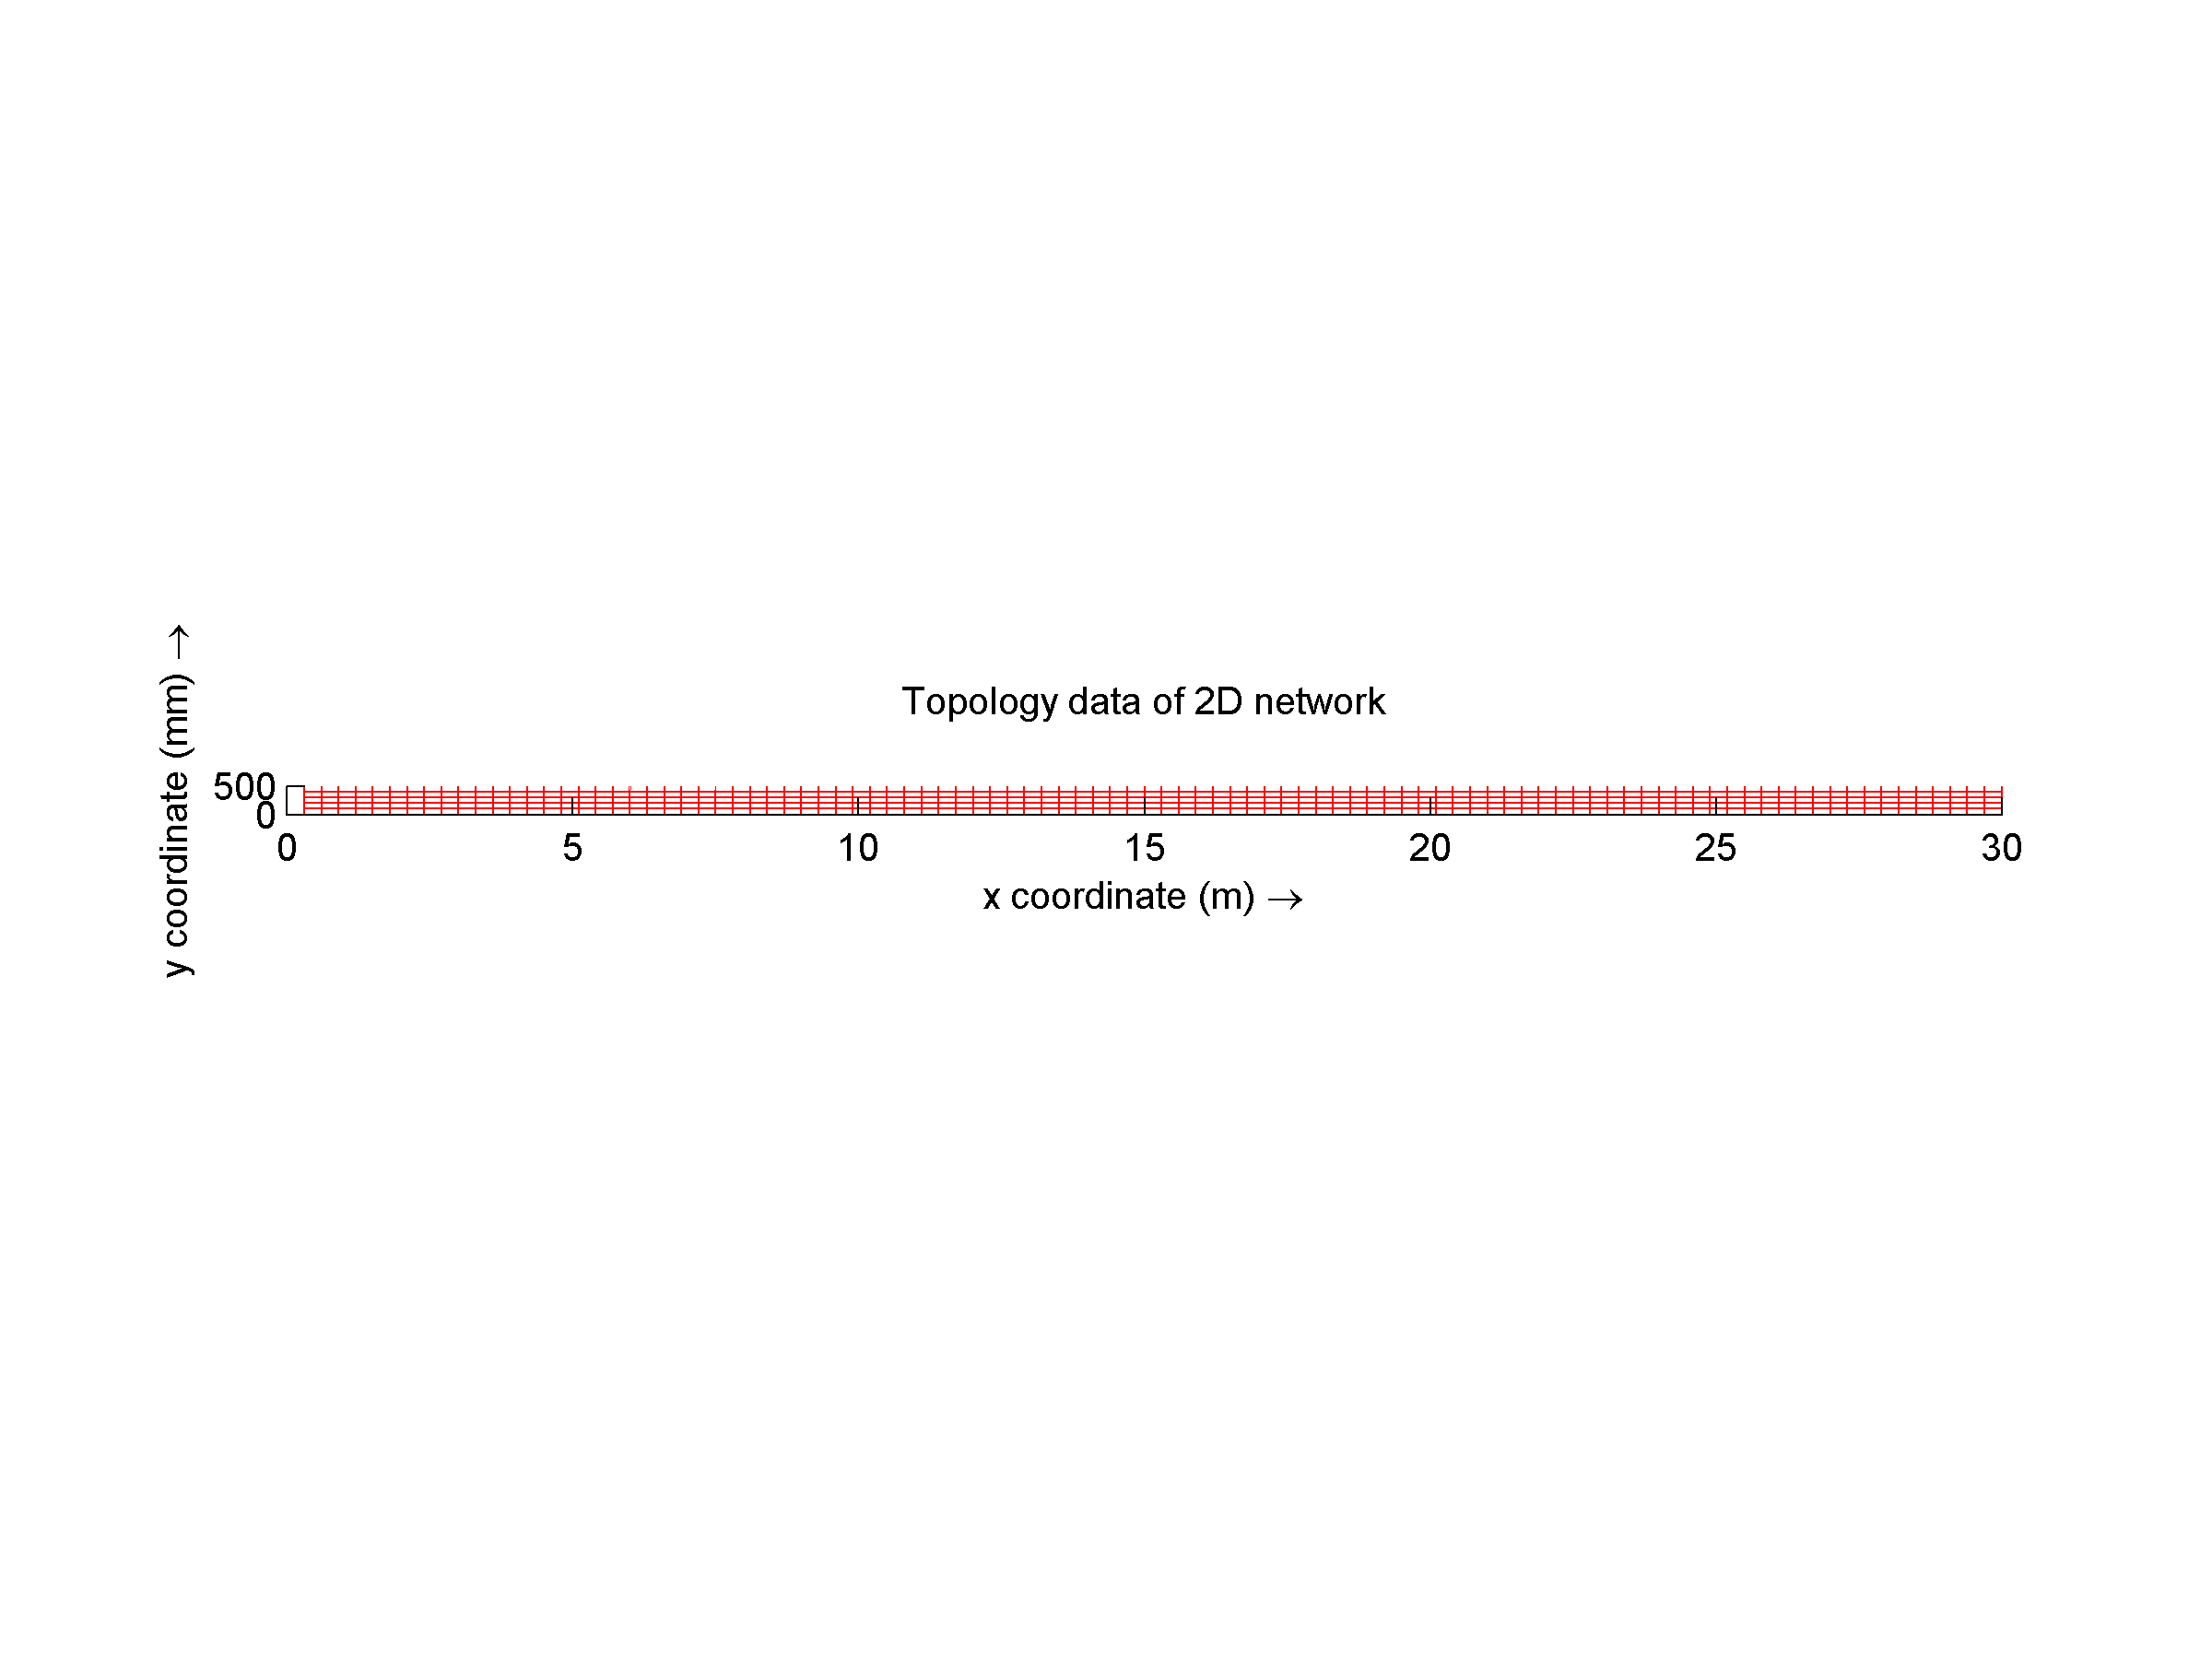
\includegraphics[width=1.0\columnwidth]{figures/T1net.png}
	\end{center}
	\caption{The network used to test the dredging-dumping.}
	\label{fig:T1-net}
\end{figure}

The testcases concern a straight channel flow with a constant roughness factor under equilibrium flow conditions. A discharge $Q$ equal to 0.09945 m$^3$/s is prescribed as an upstream boundary condition. The longitudinal bottom slope $i_b$ is prescribed to be $0.012$ (see figure (\ref{fig:initialized})). The width of the channel is 0.5 m . The white-Colebrook friction coefficient is set to 0.025 m. The downstream boundary condition is water level set to 0.00 m.The initial bed contains a trench with a width of 0.5 m, length of 5 m and a depth of 0.6 m.

\begin{figure}[h!]
	\begin{center}
		\includegraphics[width=0.7\columnwidth] {figures/initialbed.png}
	\end{center}\caption{The longitudinal cross-section of the initial bed level}
	\label{fig:initialized}
\end{figure}

Eleven test cases are tested. Every test case is performed with and without the dredging and /or dumping. The test cases are formulated to cover different cases of dredging to ensure  dredging-dumping functions work in the FM-mor module. The test cases are:
\begin{itemize}
	\item[$\bullet$] c35: Dredging and dumping the dredged material inside the model domain.
	\item[$\bullet$] c36: Dredging and dumping the dredged material outside the model domain
	\item[$\bullet$] c37: Dredge from two location and dump the dredged material at one location  inside  the model domain.
	\item[$\bullet$] c38: Dredging  and dumping the dredged material inside  the model domain at the same location. 
	\item[$\bullet$] c39: Dredging, dumping the dredged material in two locations and sand mining inside  the model domain. 
	\item[$\bullet$] c40: Dredging and dumping the dredged material inside the model  with layered bed composition. Reference test case is c35.
	\item[$\bullet$] c41: Dredging and dumping the dredged material outside the model with layered bed. Reference test case is c36.
	\item[$\bullet$] c42: Dredge from two location and dump the dredged material at one location  inside  the model with layered bed composition. Reference test case is c37.
	\item[$\bullet$] c43: Dredging  and dumping the dredged material inside  the model domain at the same location with layered bed. Reference test case is c38.
	\item[$\bullet$] c44: Dredging, dumping the dredged material in two locations and sand mining inside  the model domain with layered bed. Reference test case is c39.
	\item[$\bullet$] c45: Dredging and dumping the dredged material inside the model domain using unstructured grid (triangles). Reference test case is c35.
	\item[$\bullet$] c46: sediment nourishment inside the model domain using structured grid .
\end{itemize}
Based on the above,  test-cases are mainly divided into two parts:
\begin{itemize}
	\item[$\bullet$] test-cases with one mixed layer (c35 to c39)- structured grid.
	\item[$\bullet$] test-cases with two under layers (c40 to c44) - structured grid.
	\item[$\bullet$] test-case with one mixed layer (c45) - unstructured grid. The reference case is c35.
	\item[$\bullet$] test-case with one mixed layer to test the nourishment function (c46) - structured grid . 
\end{itemize}

\paragraph*{Test-cases with one mixed layer (structured grid)}
\subparagraph*{c35-testcase}:

The default parameters in the morphological setup are mainly used.Nevertheless, in the following part  important related setup of morphology and sediment files used are described as follows:
\begin{itemize}
	\item[$\bullet$] Sediment file $<*.sed>$:
\end{itemize}

\begin{verbatim}
[Sediment]
SedTyp           = Sand       # Must be "sand", "mud" or "bedload"
SedDia           = 1.4e-004   # [m] Median sediment diameter (D50)
TraFrm           = -1
Name             = #Van Rijn (1993)#
\end{verbatim}
$SedTyp$ is sand,
sediment transport equation is the default formula (Van Rijn (1993)),
sediment size ($D_{50}$) is equal to 0.14 mm.
\begin{itemize}
	\item[$\bullet$] Morphology file $<*.mor>$:
\end{itemize}
The morphological update $ MorUpd$ and bed composition update  $CmpUpd$ are switched on. $MorFac$ is equal to 180 and the spin-up interval from the start time until the start of morphological changes $MorStt$ is 5 minutes.
Dredging and dumping polygon is prepared  according to the itemize of every simulation setup. For instance in $c35$ simulation two polygons were prepared one for the dredging area and the other one for the dumping area.  The dredging file (dad file) is prepared as follows:
\begin{verbatim}
[DredgeFileInformation]
FileCreatedBy     = WL | DH, Delft3D-QUICKIN V: 4.11.00; Feb 2004
FileCreationDate  = 15:32:06, 05-03-2004
FileVersion       = 01.02
PolygonFile       = dredge.pol
[Dredge]
Name              = KUIL
DredgeDepth 	  =   0.60
Dump        	  = BULT
Percentage   	  = 100.0
\end{verbatim}

The area of  dredging called (KUIL) and the model has to maintain a depth of 0.6 m in the area. All the dredged material must be dumped on the dump area (BULT). Both areas within the model domain as shown in  figure (\ref{fig:C35dad}).

\begin{figure}[h!]
	\begin{center}
		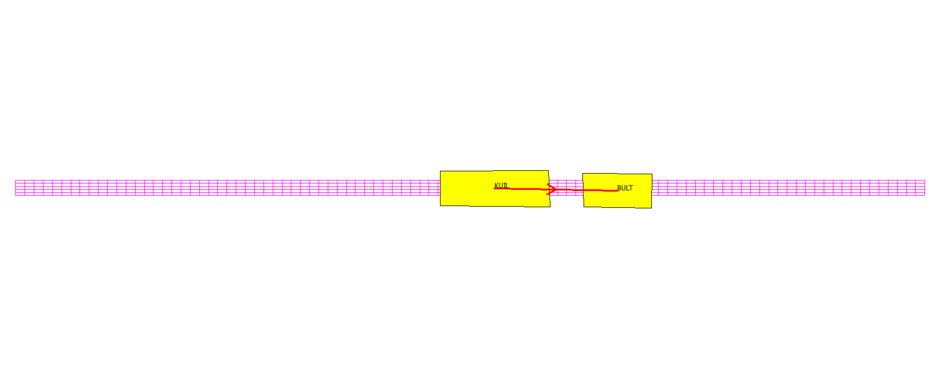
\includegraphics[width=0.7\columnwidth] {figures/c35dad.png}
	\end{center}\caption{Plan view of dredging and dumping areas  inside the model domain in C35 simulation}
	\label{fig:C35dad}
\end{figure}

\begin{figure}[h!]
	\begin{center}
		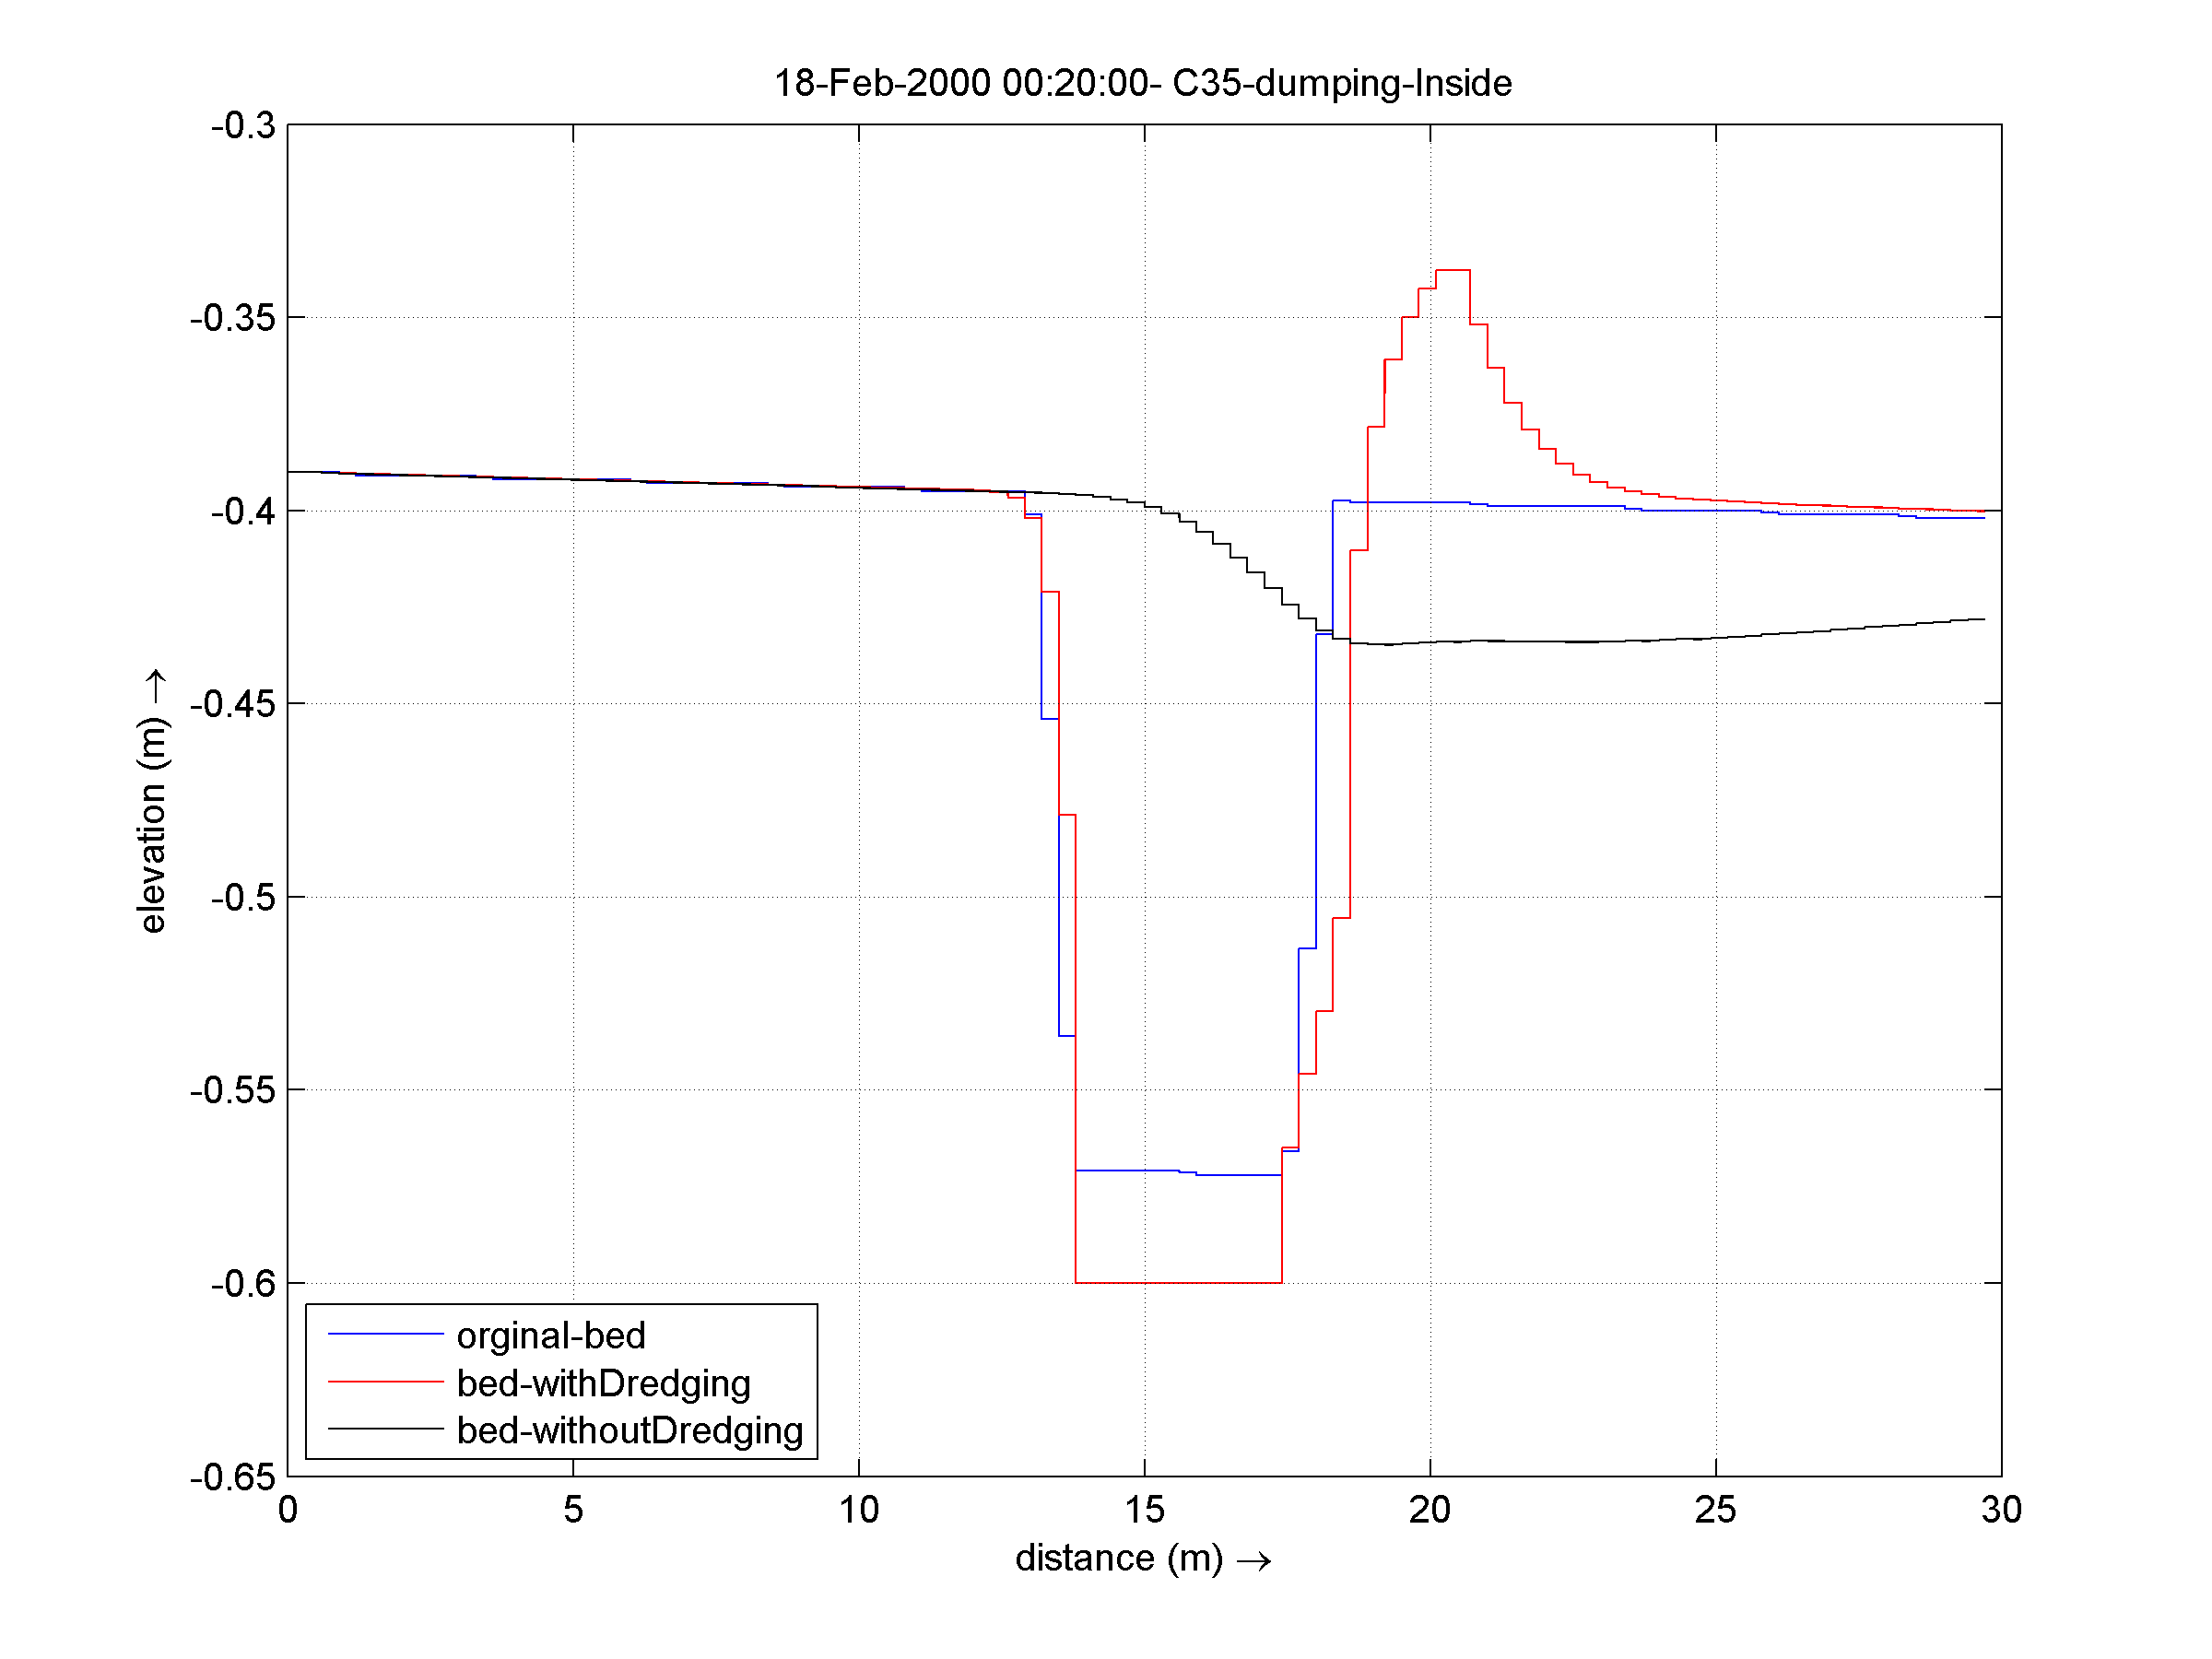
\includegraphics[width=0.7\columnwidth] {figures/C35-bedComparison.png}
	\end{center}\caption{he result of $c35$ test-case with and without dredging and dumping}
	\label{fig:C35-bedComparison}
\end{figure}

Another simulation is setup but without dredging and dumping to compare it with the above-mentioned simulation which includes dredging and dumping. The result shows that the model  dredges  sediment to keep the 0.6 m  water depth at the specified location and dump the material at  dumping area (BULT) as shown in figure (\ref{fig:C35-bedComparison}). The figure illustrates  bed level change at the longitudinal centerline cross section of the model domain.

\subparagraph*{c36-testcase}:

the test-case number c36 is similar to $c35$ except that the dumping in c36 is outside the model domain not inside. Figure (\ref{fig:C36-bedComparison}) shows that the model keeps dredging to maintain the 0.6 m depth at the designated area, while the simulation without dredging provides different bed level change.
\begin{figure}[h!]
	\begin{center}
		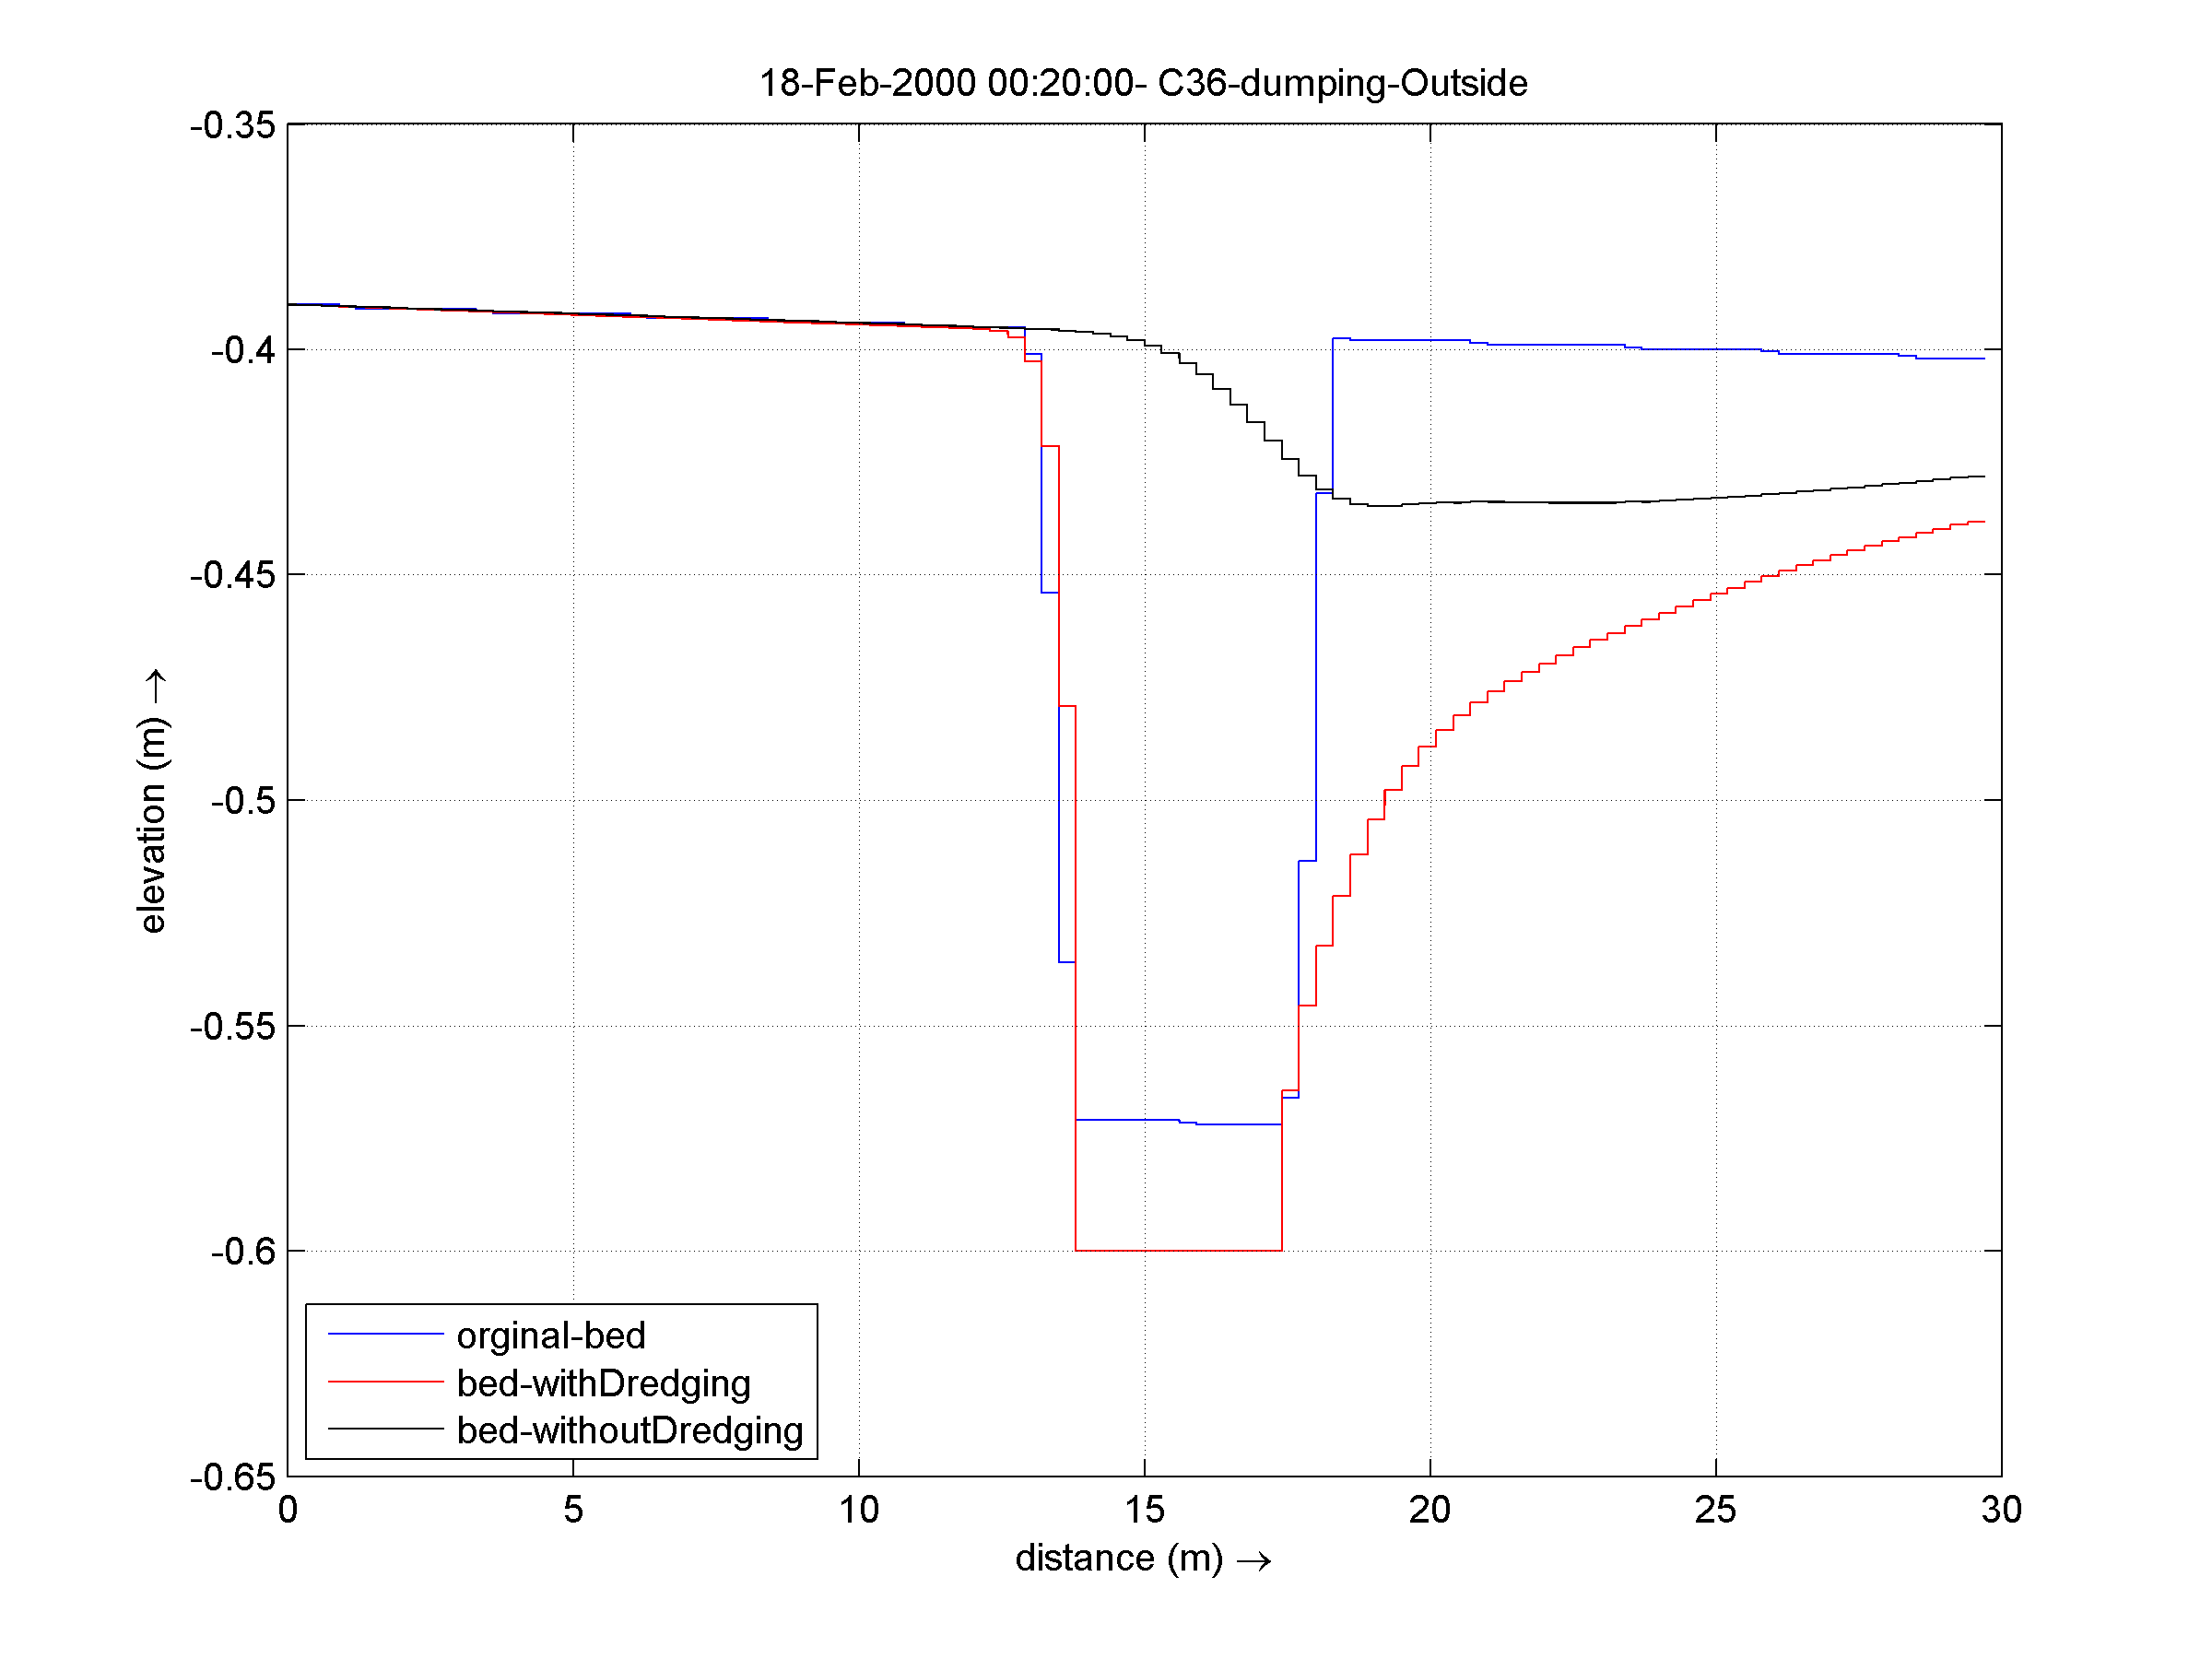
\includegraphics[width=0.7\columnwidth] {figures/C36-bedComparison.png}
	\end{center}\caption{The result of $c36$ test-case with and without dredging and dumping}
	\label{fig:C36-bedComparison}
\end{figure}

\subparagraph*{c37-testcase}:

In the test case number c37 the dumping area is divided into two adjacent dredging areas with same dimension as the  dredging area in c35 and c36. The reasoning behind that is to check whether the model provides similar bed level change as c35 (see figure (\ref{fig:C37dad})). The dredging-dumping file (dad file) used is illustrated below.
\begin{verbatim}
[DredgeFileInformation]
FileCreatedBy    = WL | DH, Delft3D-QUICKIN V: 4.11.00; Feb 2004
FileCreationDate = 15:32:06, 05-03-2004
FileVersion      = 01.02
PolygonFile      = dredge.pol
[Dredge]
Name         	 = KUIL1
DredgeDepth	     =   0.60
Dump        	 = BULT
Percentage 	     = 100.0
[Dredge]
Name      	     = KUIL2
DredgeDepth	     =   0.60
Dump       	     = BULT
Percentage  	 = 100.0
\end{verbatim}

\begin{figure}[h!]
	\begin{center}
		\includegraphics[width=0.7\columnwidth] {figures/C37dad.png}
	\end{center}\caption{c37 dumping and dredging locations}
	\label{fig:C37dad}
\end{figure}

The result shows that the dumping and dredging process gives similar behavior as c35 (compare  figure (\ref{fig:C37-bedComparison-Dredge(2)-dump(1)}).

\begin{figure}[h!]
	\begin{center}
		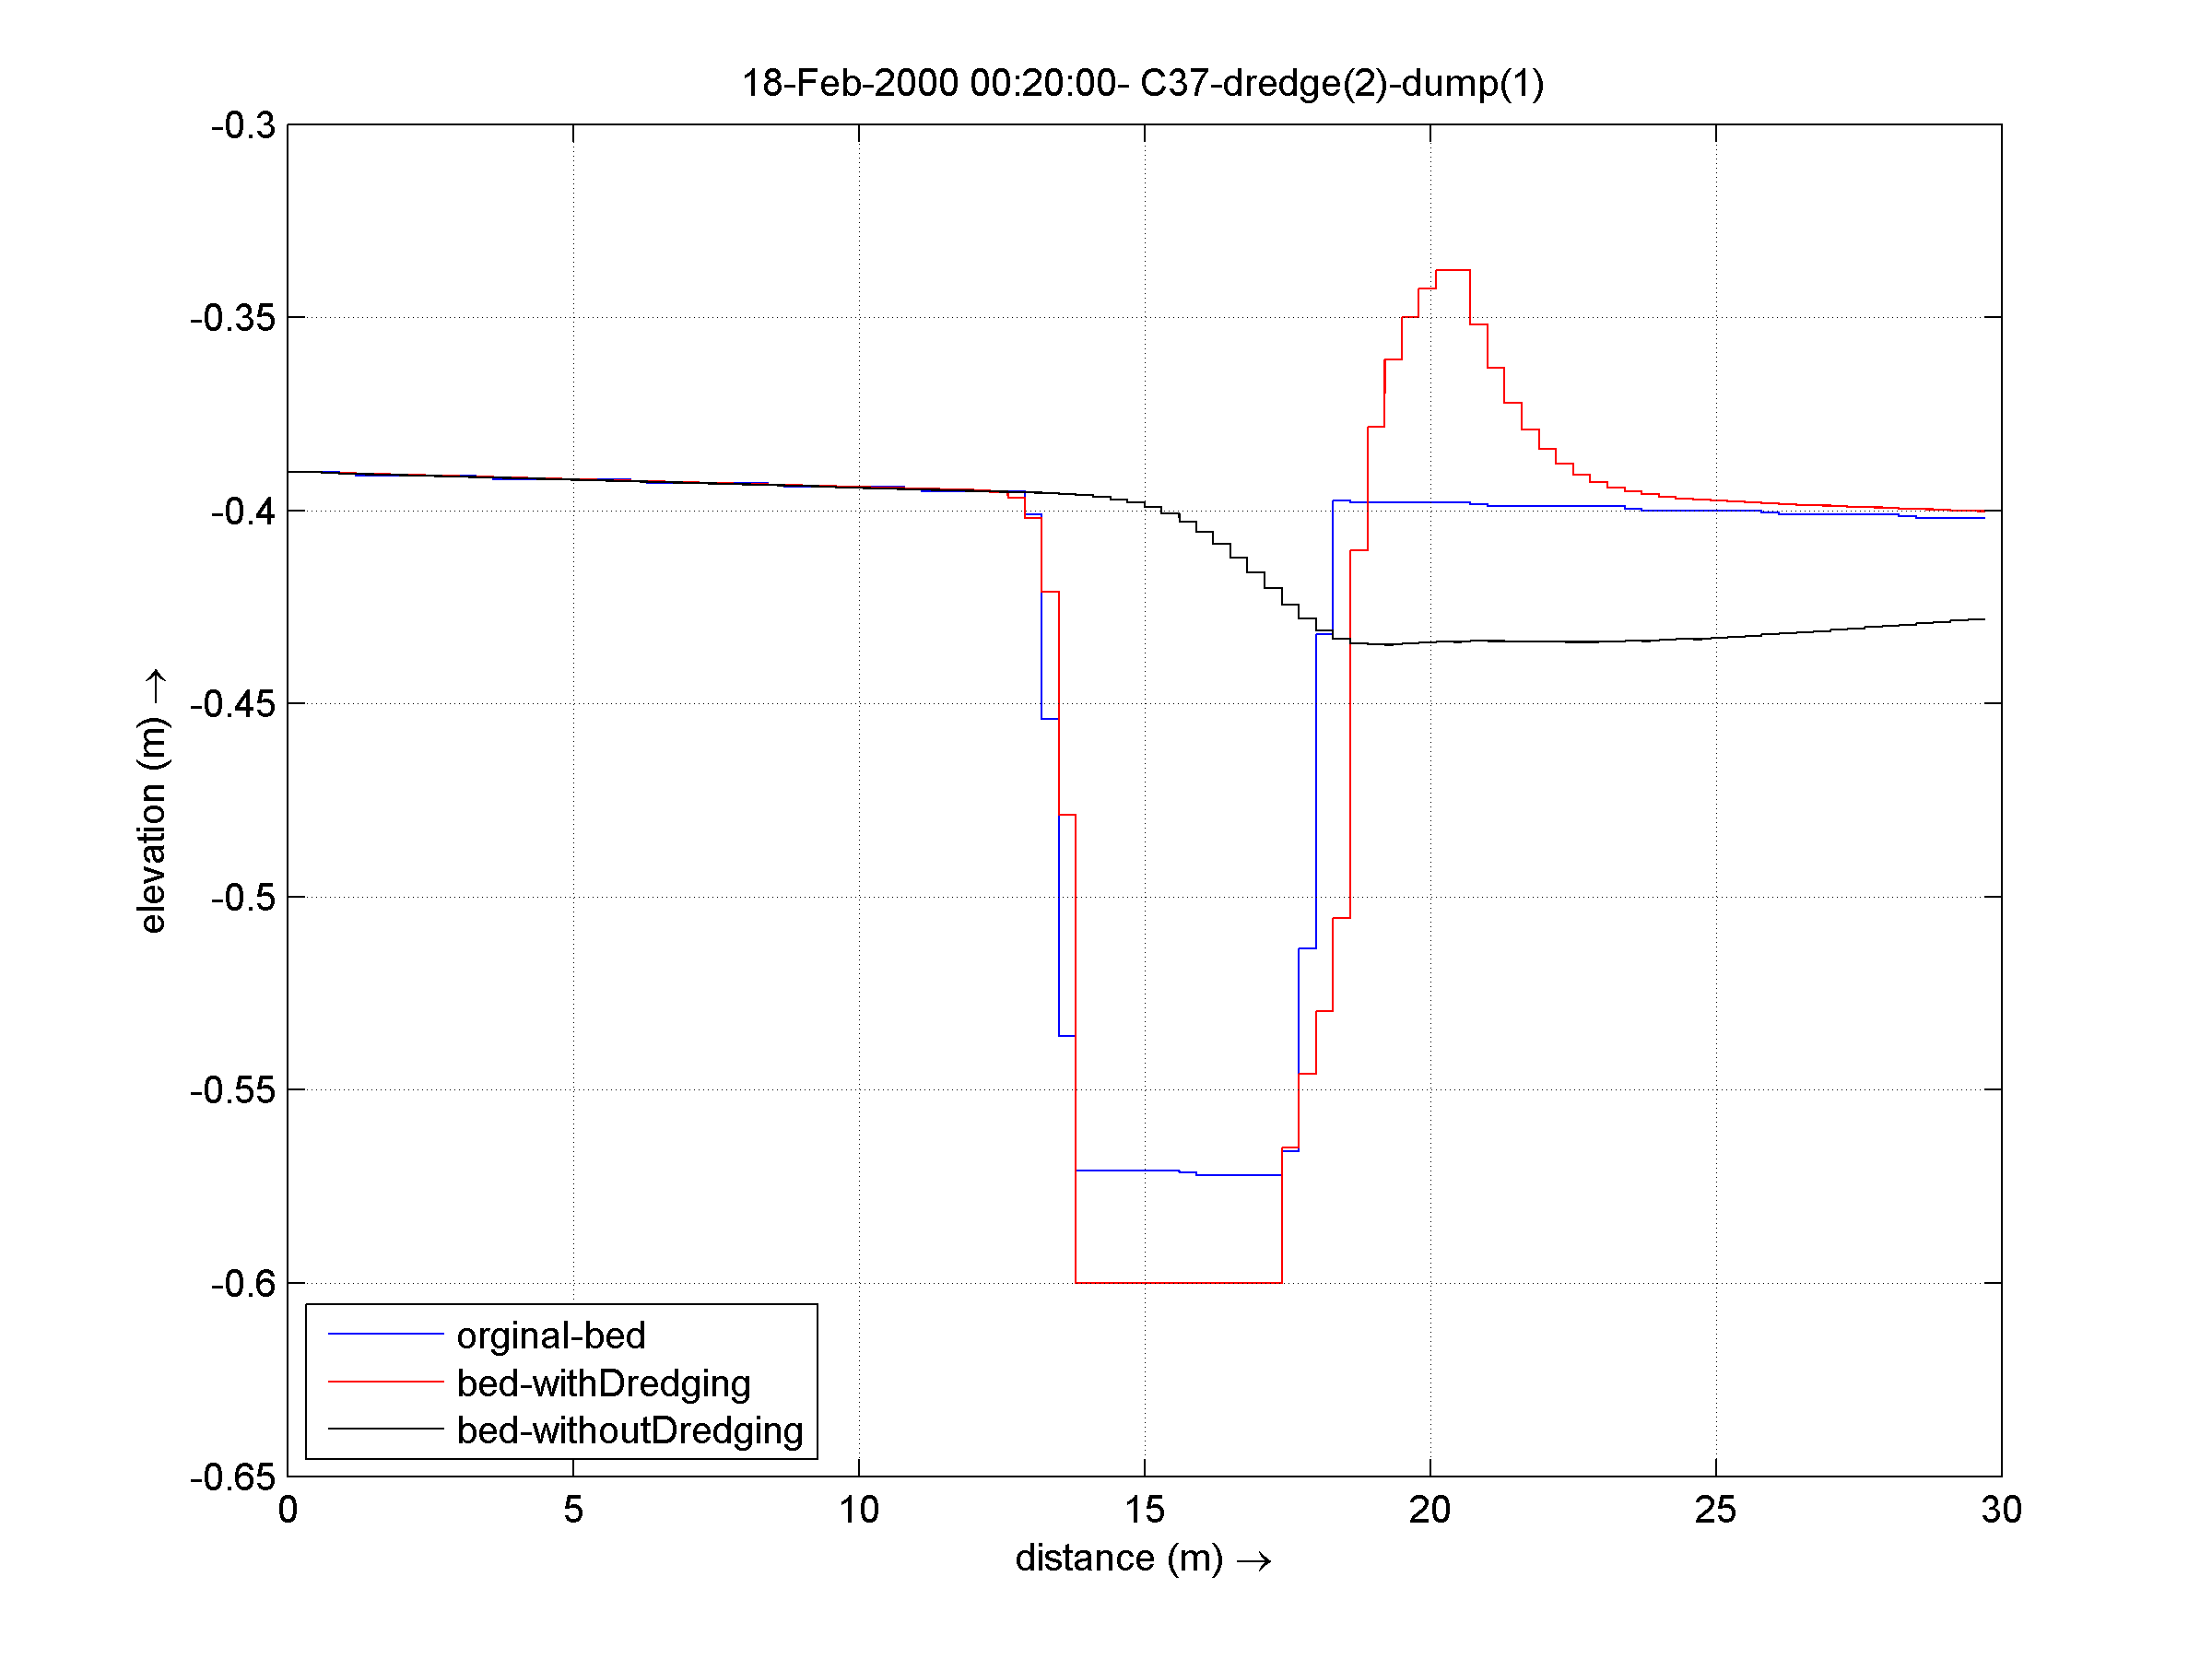
\includegraphics[width=0.7\columnwidth]{figures/C37-bedComparison-Dredge(2)-dump(1).png}
	\end{center}\caption{c37- bed level at the centerline cross section of the model domain. blue line is the original bed level, the red line is the result of simulation with dredging and the black line is the result of simulation without dredging}
	\label{fig:C37-bedComparison-Dredge(2)-dump(1)}
\end{figure}

\subparagraph*{c38-testcase}:
In this test case the dredging and dumping are at the same location. The data included in the dad file are reflected below . The remaining setup of the simulation is similar to c35 test-case.
\begin{verbatim}
[DredgeFileInformation]
FileCreatedBy    = WL | DH, Delft3D-QUICKIN V: 4.11.00; Feb 2004
FileCreationDate = 15:32:06, 05-03-2004
FileVersion      = 01.02
PolygonFile      = dredge.pol
[Dredge]
Name         	 = KUIL
DredgeDepth  	 = 0.60
Dump        	 = KUIL
Percentage  	 = 100.0
\end{verbatim}

The simulation result shows that the bed level change at the longitudinal cross-section is almost  similar to the bed changes in the simulation without dredging. The difference at dredging and dumping area might be due to the fact that  model dumps the material in an equal manner (see figure (\ref{fig:C38-bedComparison-Dredge-dump}).

\begin{figure}[h!]
	\begin{center}
		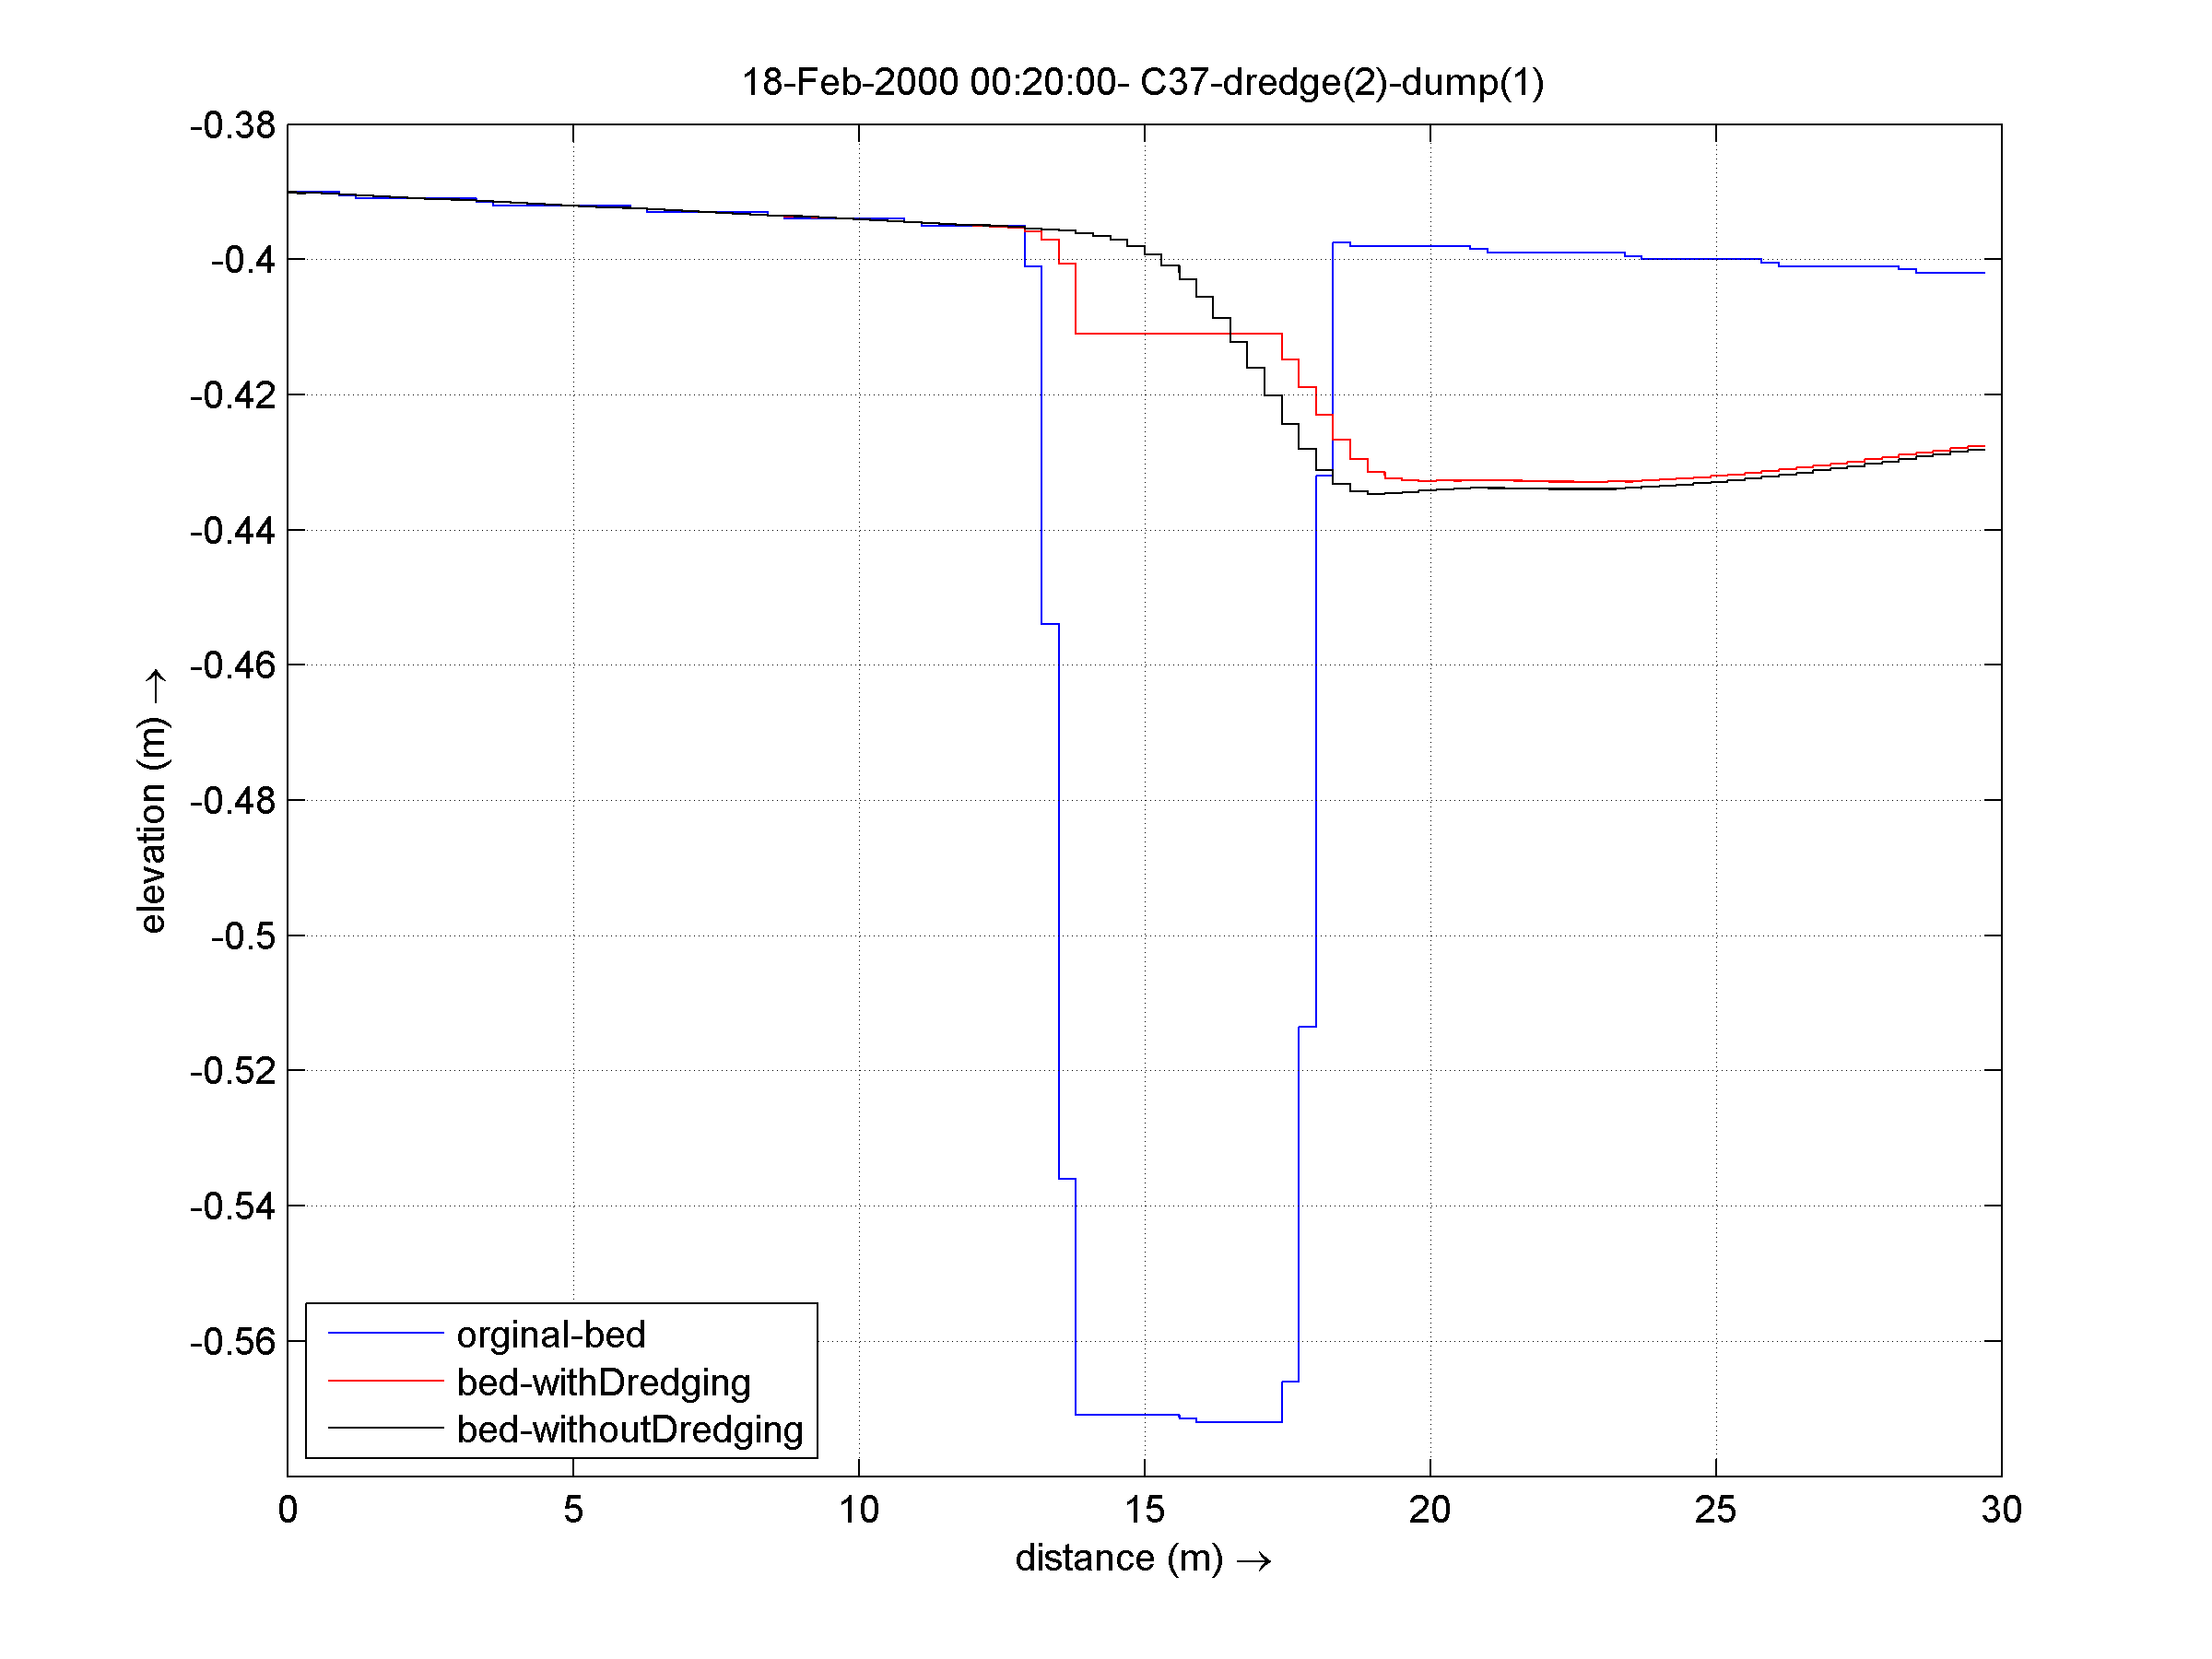
\includegraphics[width=0.7\columnwidth] {figures/C38-bedComparison-Dredge-dump.png}
	\end{center}\caption{c38- bed level at the centerline cross section of the model domain. blue line is the original bed level, the red line is the result of simulation with dredging and the black line is the result of simulation without dredging}
	\label{fig:C38-bedComparison-Dredge-dump}
\end{figure}


\subparagraph*{c39-testcase}:
In this test case  we use the other network of straight channel. A straight channel flows with a constant roughness factor under equilibrium flow conditions. A discharge $Q$ equal to 1.0 m$^3$/s is prescribed as an upstream boundary condition. The longitudinal bottom slope $i_b$ is prescribed to be $0.012$ (see figure \ref{fig:c39dad}). The length of the channel is 10 km, while the width of the channel is 100 m . The white-Colebrook friction coefficient $C$ is set to 0.025 m. The downstream boundary condition is water level set to 0.00 m.The initial bed contains a trench with a width of 0.5 m and length of 5 m.
In this test-case:
\begin{itemize}
	\item[$\bullet$] Dredging is the same as previous test-cases.
	\item[$\bullet$] Dumping is divided to be distributed in two locations. 90 percent of the dredged material is dumped in location (1), while the 10 percent is dumped in location (2).
	\item[$\bullet$] Sand mining: 250,000 m3 shall be taken from the model to be used for other purposes. 
\end{itemize}

\begin{figure}[h!]
	\begin{center}
		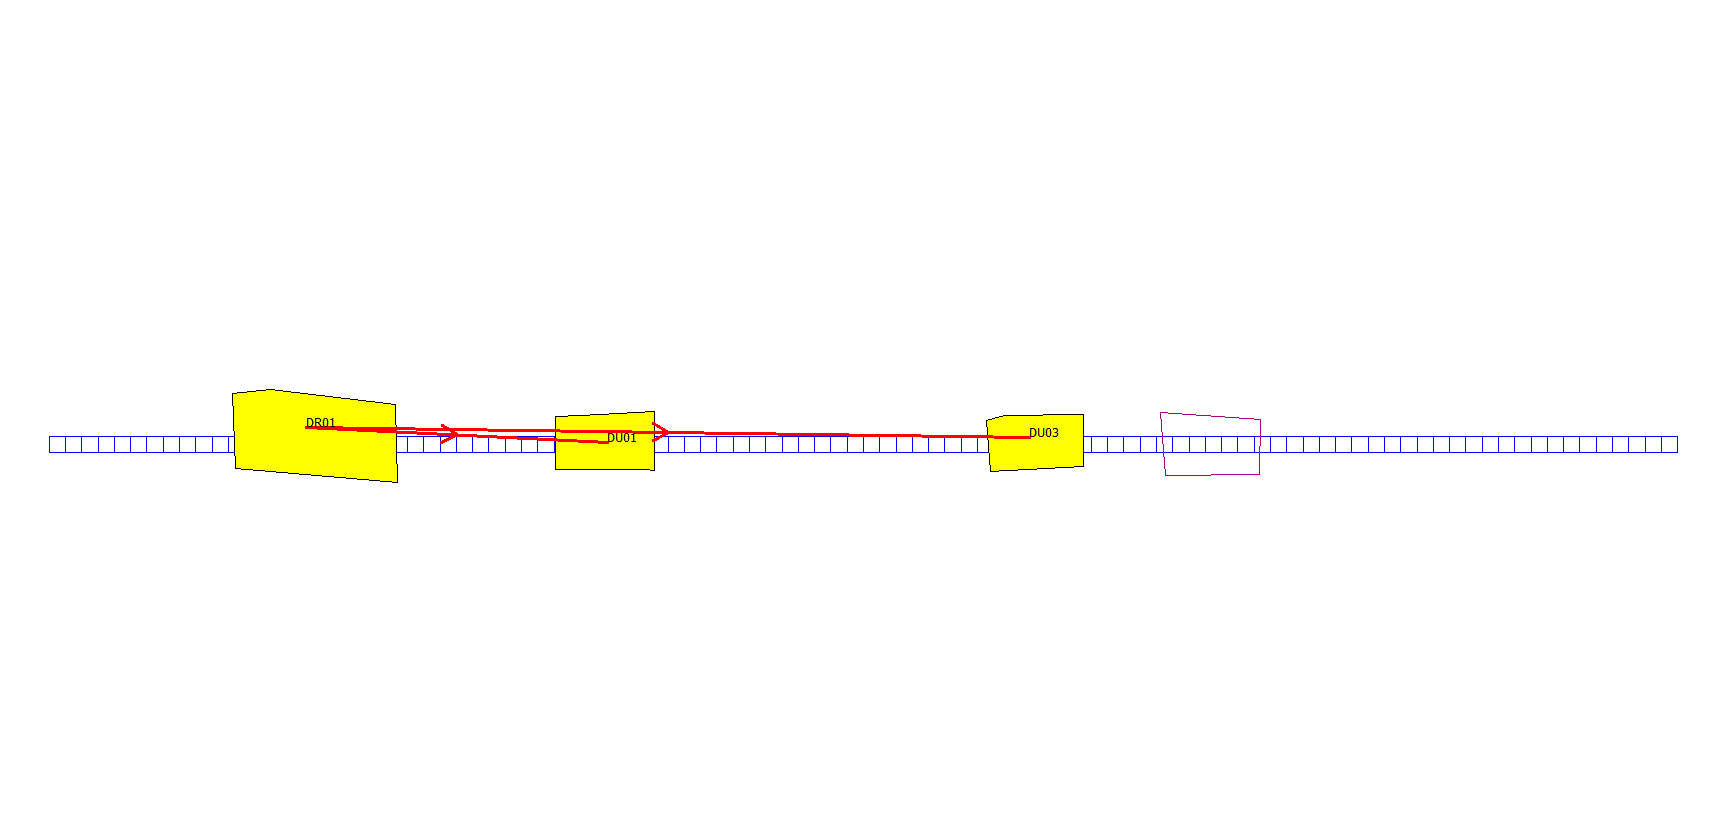
\includegraphics[width=0.7\columnwidth] {figures/c39dad.png}
	\end{center}\caption{c39 net and dredging dumping locations. The blank polygon shows the sand mining area}
	\label{fig:c39dad}
\end{figure}

The dad file information inserted to the model are:
\begin{verbatim}
[DredgeFileInformation]
FileCreatedBy    = WL | DH, Delft3D-QUICKIN V: 4.11.00; Feb 2004
FileCreationDate = 15:32:06, 05-03-2004
FileVersion      = 01.02
PolygonFile      = dad.pol
[Dredge]
Name             = DR01
DredgeDepth      = 10.0
Dump             = DU01
Percentage       =  90.0
Dump             = DU03
Percentage       =  10.0
[Sandmining]
Name             = SM01
Volume           = 2500000.0 
\end{verbatim}

In addition to that, instead of using one-grain size of sediment $(d50)$ , a file of variable sediment grain size, distributed spatially, is used. The result of  bed level shows that the dredging and dumping is performed relatively well. and the sand for mining is also taken from the model domain as shown in figure (\ref{fig:C39-bedComparison-sandmining}).

\begin{figure}[h!]
	\begin{center}
		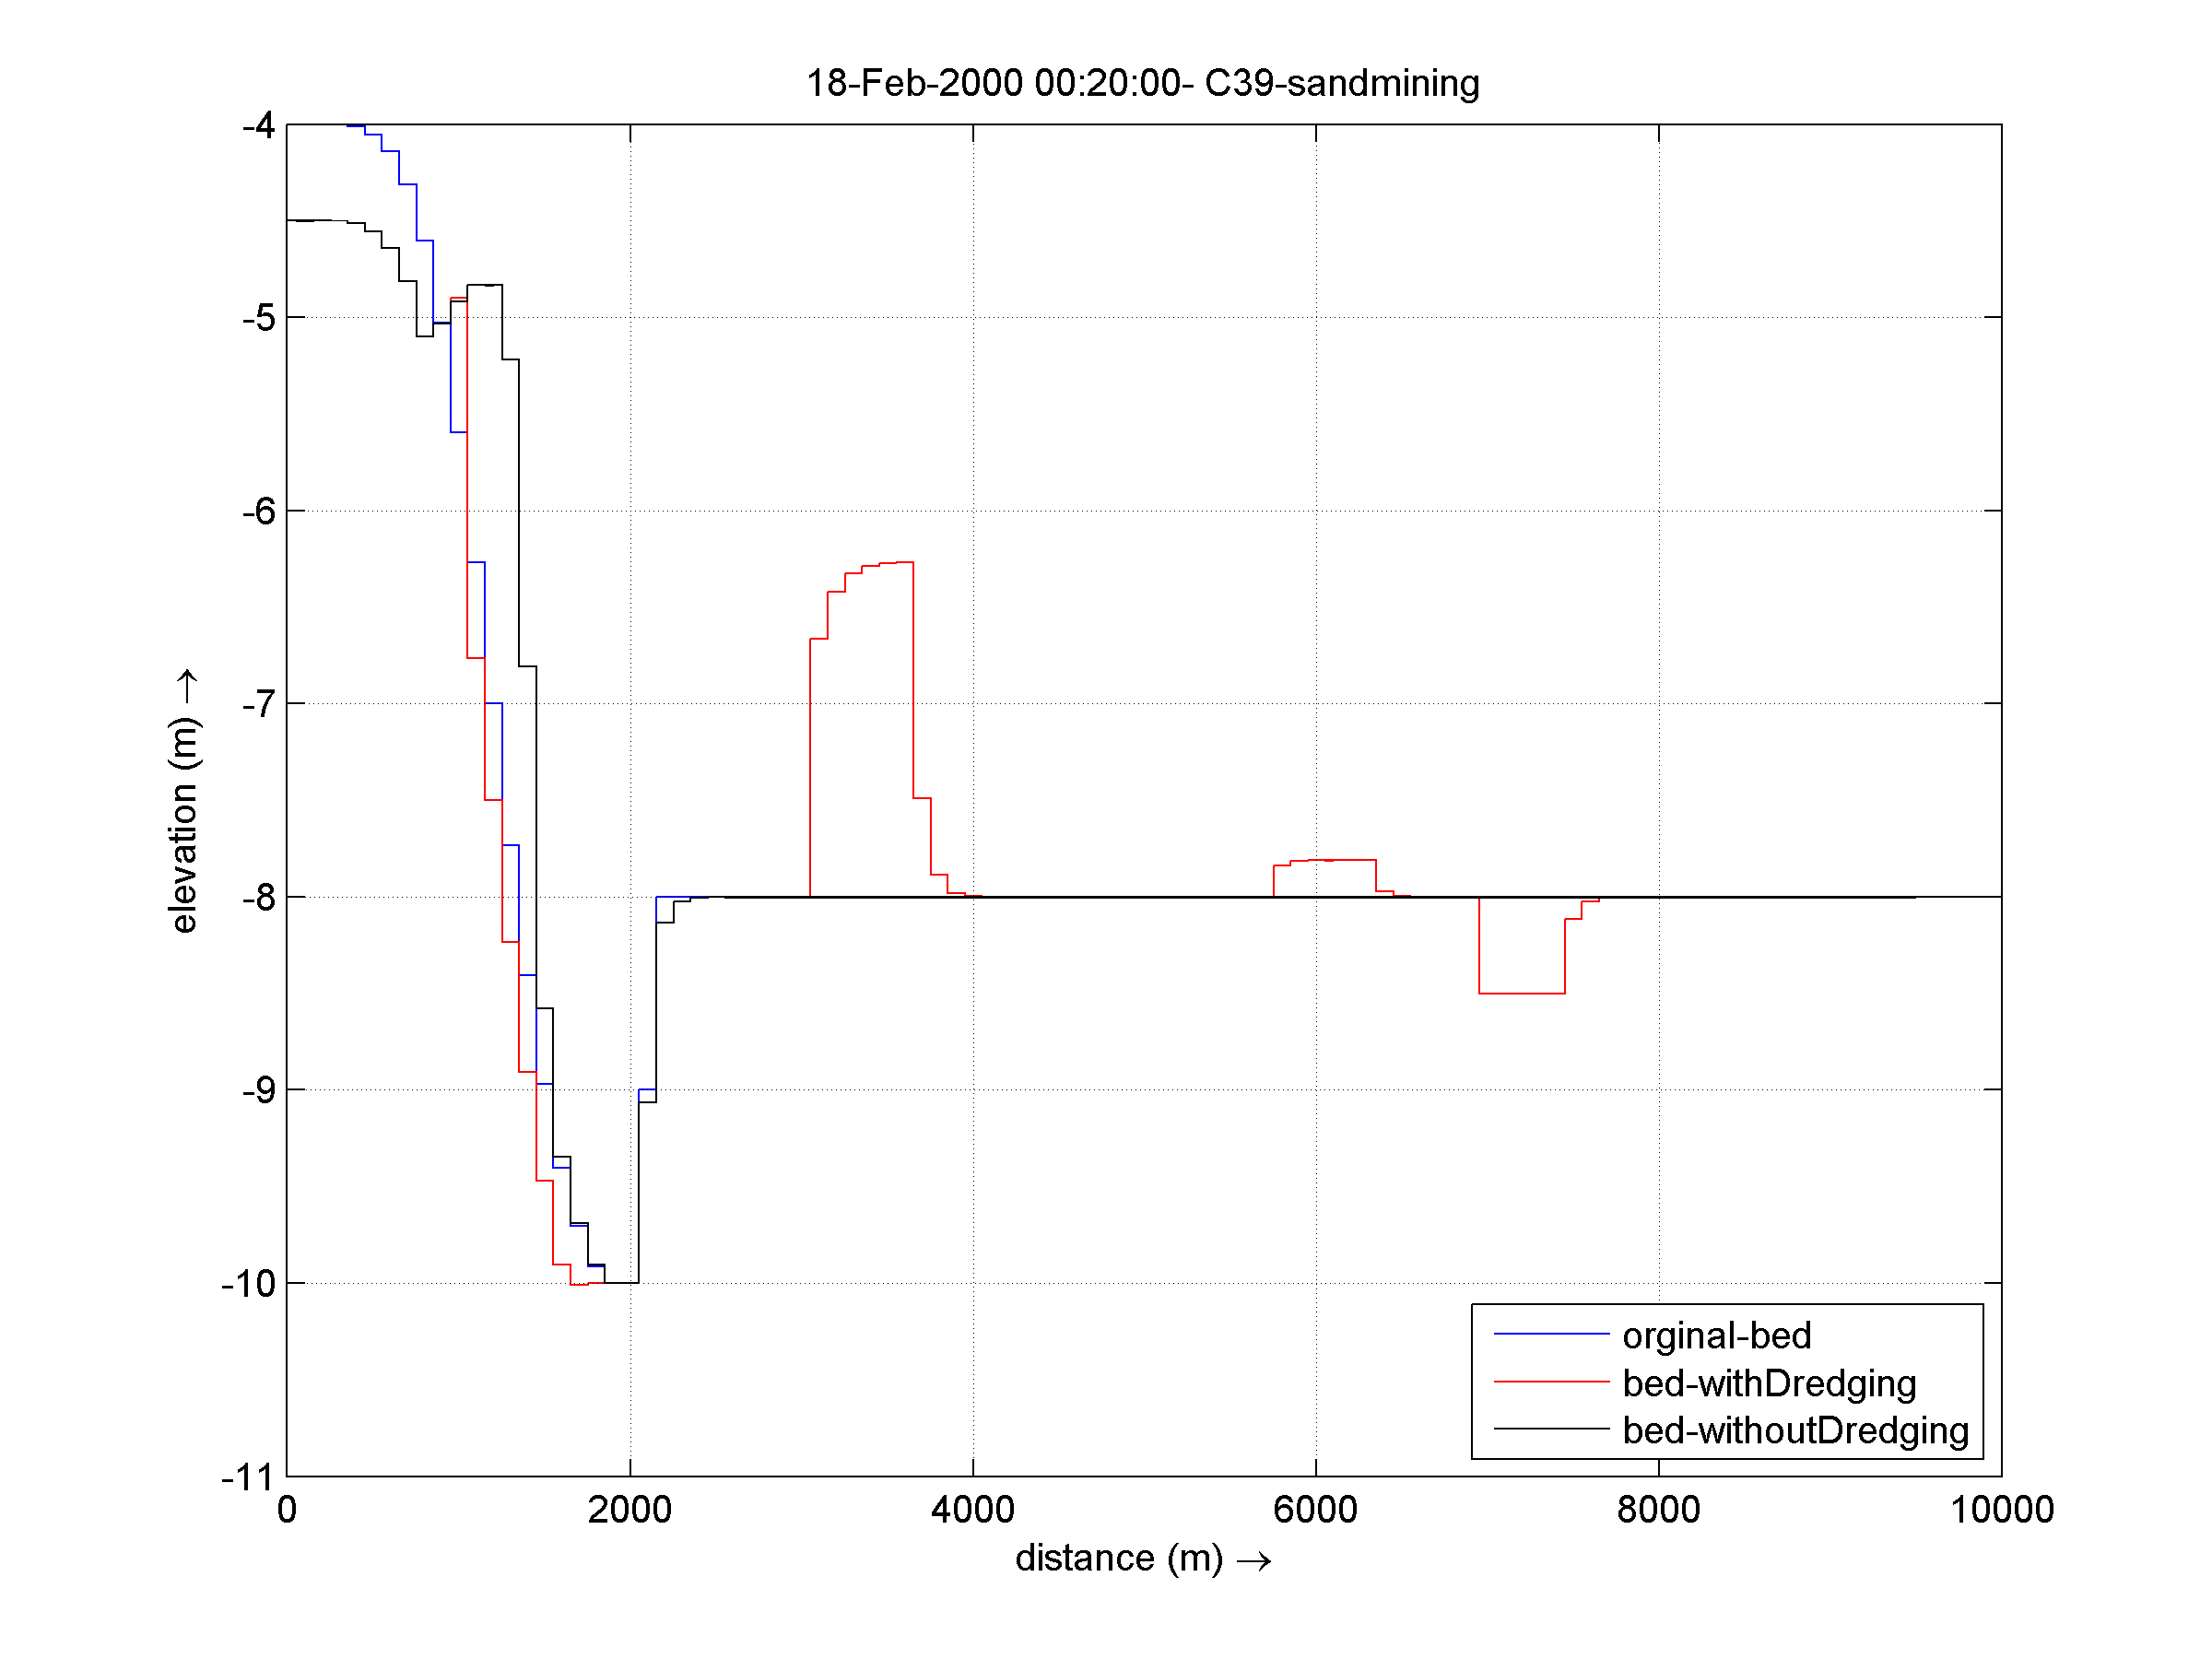
\includegraphics[width=0.7\columnwidth] {figures/C39-bedComparison-sandmining.png}
	\end{center}\caption{c39- bed level at the centerline cross section of the model domain. blue line is the original bed level, the red line is the result of simulation with dredging and the black line is the result of simulation without dredging}
	\label{fig:C39-bedComparison-sandmining}
\end{figure}

\paragraph*{Test-cases with two under layer (structured grid)}
In this section all the above test-cases are rerun but with switching on under-layering function. Furthermore,Three types of sediment are used. The purpose behind that is to check whether the dredging and dumping is working well also with under-layering function or not. The sediment file is modified for all of the following test-cases as follows:
\begin{verbatim}
[[SedimentFileInformation]
FileCreatedBy     = Delft3D FLOW-GUI, Version: 3.56.29165         
FileCreationDate  = Wed Jan 07 2015, 16:31:07         
FileVersion       = 02.00                        
[SedimentOverall]
Cref              =  1.0000000e+006 [kg/m3] CSoil Reference density 
IopSus            = 0 , If Iopsus = 1: susp. sediment
[Sediment]
Name              = #Sediment1#    Name of sediment fraction
SedTyp            = sand           Must be "sand", "mud" or "bedload"
RhoSol            =  2.6500000e+003    [kg/m3]  Specific density
SedDia            =  1.2000000e-004    [m] Median sediment diameter (D50)
CDryB             =  1.6000000e+003    [kg/m3] Dry bed density
IniSedThick       =  5.0000000e-001    [m] Initial sediment layer Thichness
FacDSS            =  1.0000000e+000    [-] FacDss * SedDia = Initial SS Dia  
[Sediment]
Name              = #Sediment2#   Name of sediment fraction
SedTyp            = sand          Must be "sand", "mud" or  "bedload"
RhoSol            =  2.6500000e+003    [kg/m3] Specific density
SedDia            =  2.0000000e-004    [m] Median sediment diameter (D50)
CDryB             =  1.6000000e+003    [kg/m3] Dry bed density
IniSedThick       =  5.0000000e-001    [m] Initial sediment layer thickness
FacDSS            =  1.0000000e+000    [-] acDss * SedDia = Initial SS Dia
[Sediment]
Name              = #Sediment3#    Name of sediment fraction
SedTyp            = sand           Must be "sand", "mud" or "bedload"
RhoSol            =  2.6500000e+003    [kg/m3] Specific density
SedDia            =  3.0000000e-004    [m] Median sediment diameter (D50)
$CDryB$           =  1.6000000e+003    [kg/m3] Dry bed density
IniSedThick       =  5.0000000e-001    [m] Initial sediment layer  thickness 
FacDSS            =  1.0000000e+000    [-]
\end{verbatim}
In addition, the following part is added to the morphology file to activate the under-layer function and the hindering and exposure  in the following test cases.
\begin{verbatim}
HidExp           = true
$Dm$             = true
Percentiles      = 10 50 90
[underlayer]
IUnderLyr        =  2
MxNULyr          = 5        Number of bookkeeping layers
ThTrLyr          = 1    [m] Thickness transport layer
ThUnLyr          = 2    [m] Thickness of bookkeeping layers

\end{verbatim}

\subparagraph*{c40-test-case}:

In this test case the setup is similar to c35 except the graded sediments and the under-layer function. Result of  bed level change is illustrated in figure (\ref{fig:C40-bedComparison-dredgedumpIn}).

\begin{figure}[h!]
	\begin{center}
		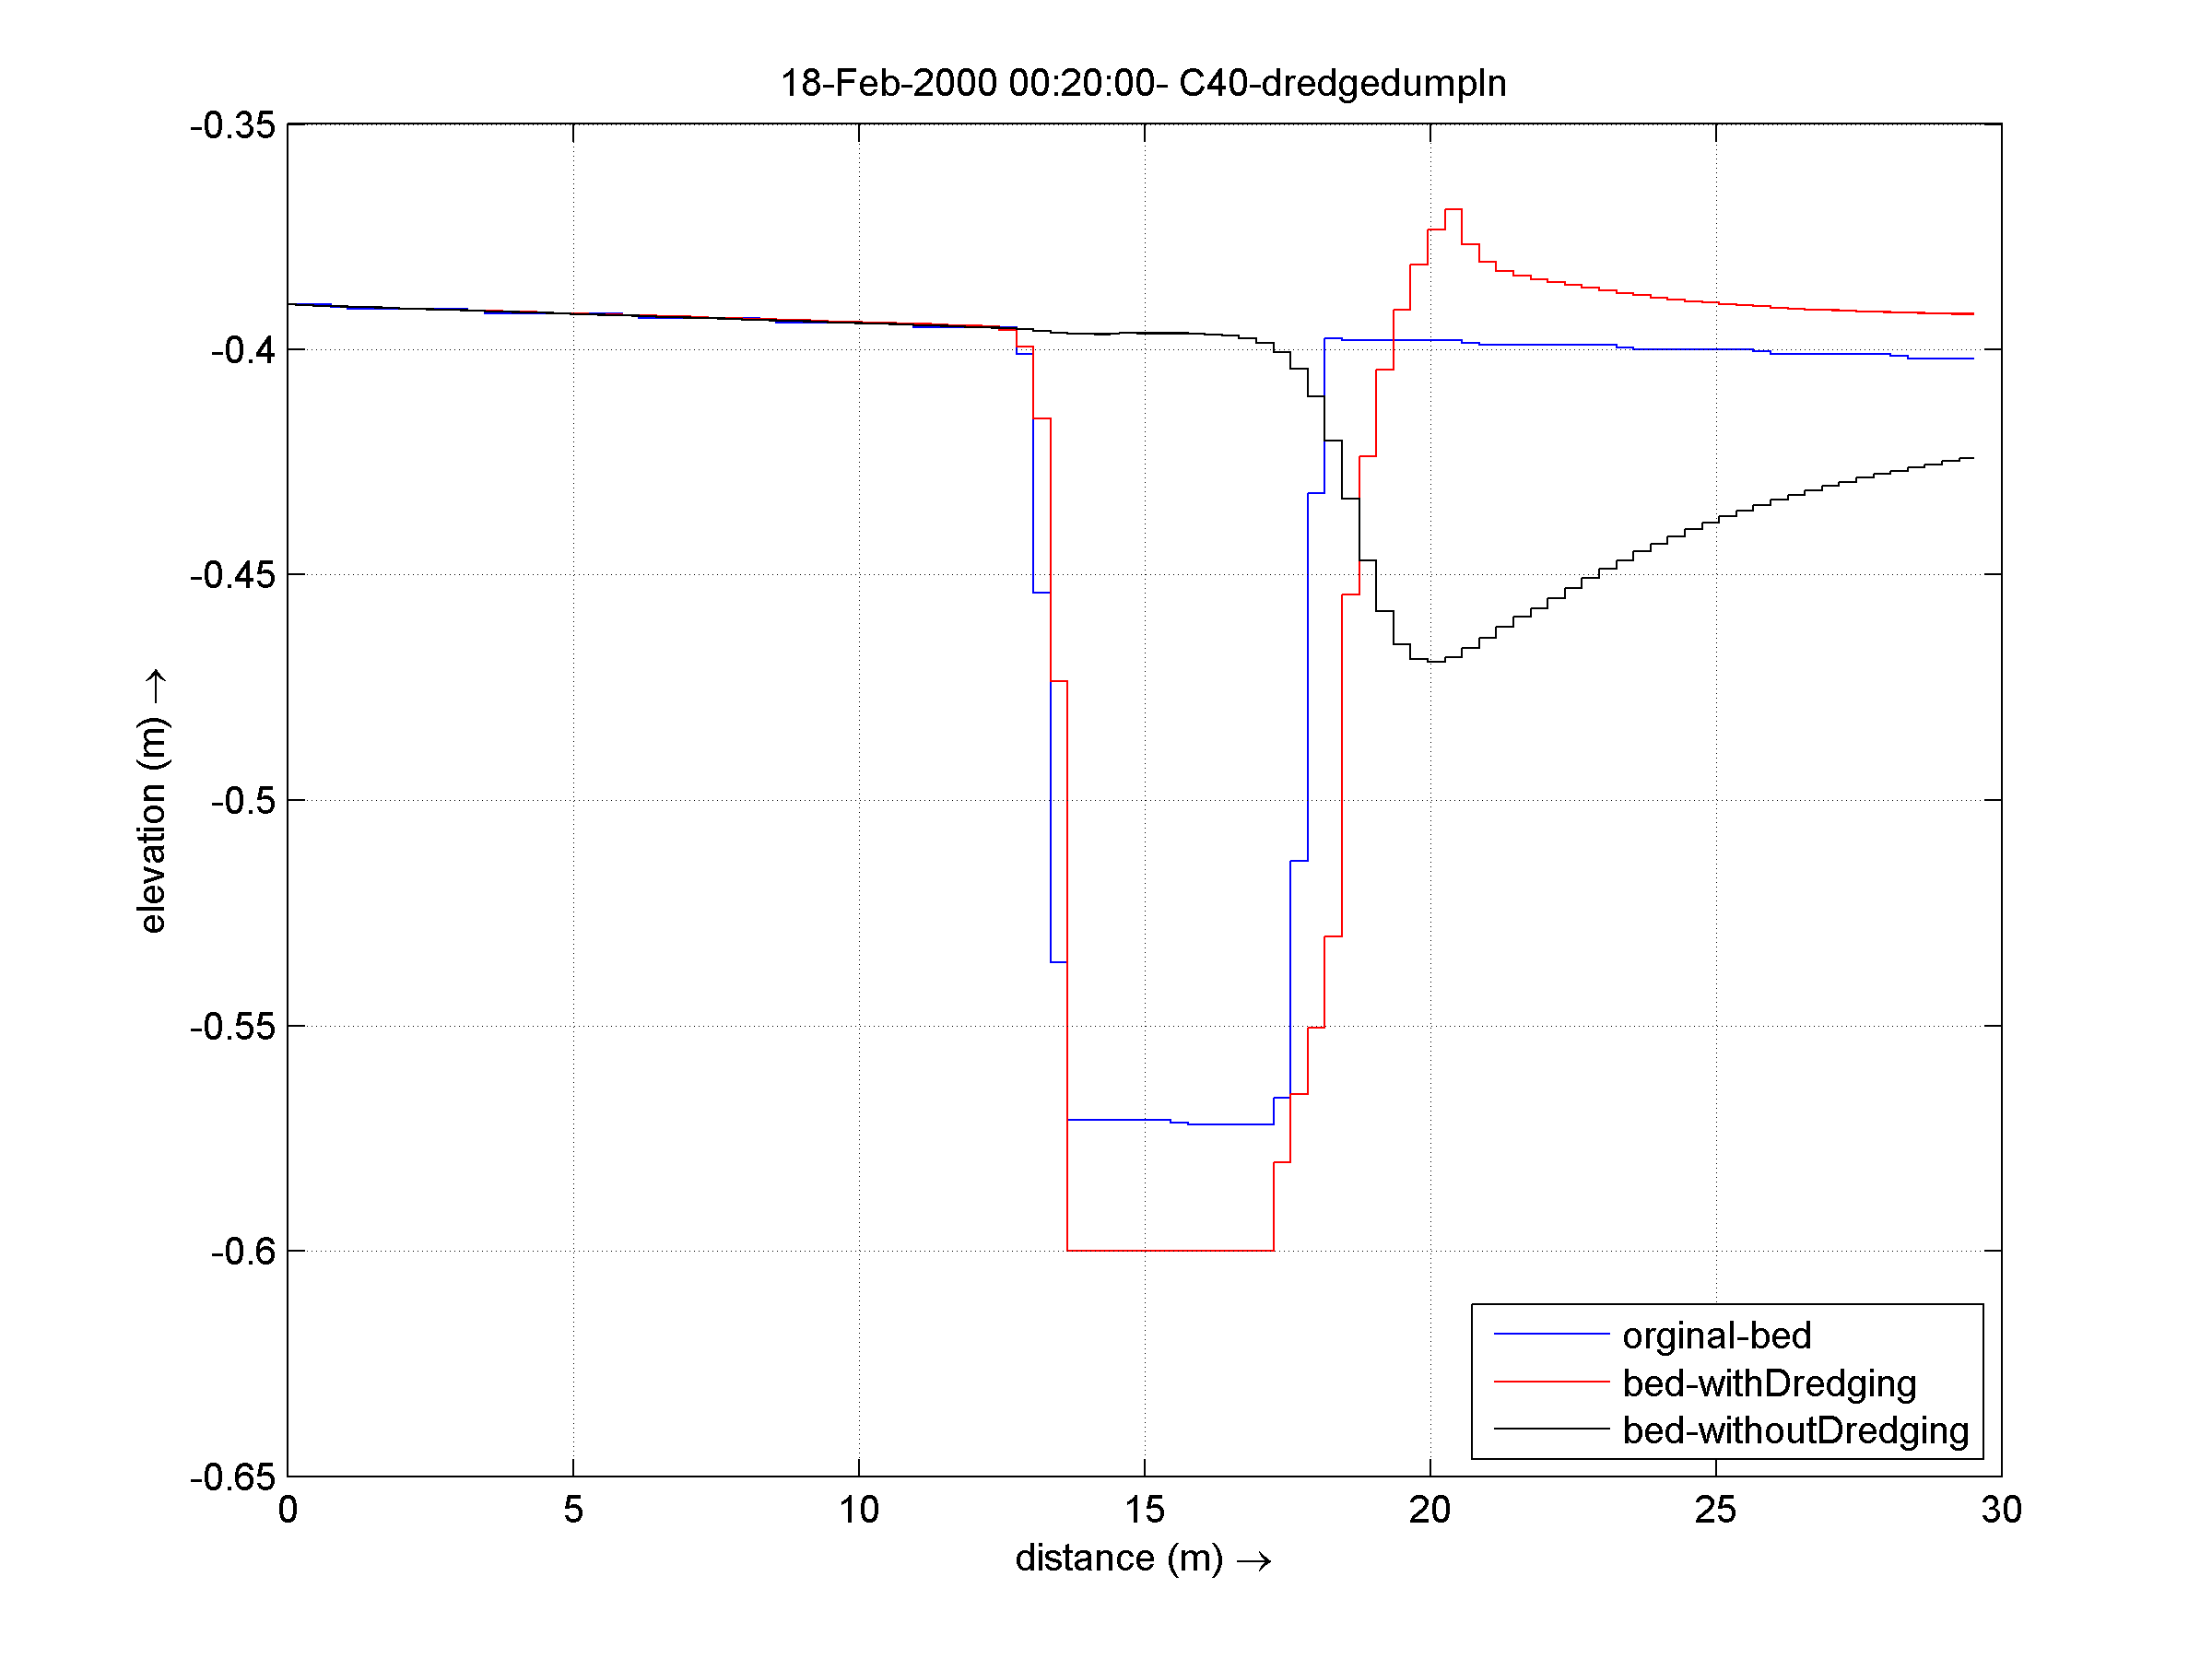
\includegraphics[width=0.7\columnwidth]{figures/C40-bedComparison-dredgedumpIn.png}
	\end{center}\caption{c40- bed level at the centerline cross section of the model domain. blue line is the original bed level, the red line is the result of simulation with dredging and the black line is the result of simulation without dredging}
	\label{fig:C40-bedComparison-dredgedumpIn}
\end{figure}

The figure shows a comparison between the original bed level and the bed with dredging and the bed without dredging. The trend is relatively similar to c35 results. However, the magnitude of bed aggradation and degradation at the dumping location (between 18.5 m to 25 m distance along the x-axis) is more than c35. This may need further investigation.

\subparagraph*{c41,c42,c43 and c44-test-case}:

Those test cases produce similar the results as c40. The dredging and dumping functions perform well, but the magnitude of bed aggradation and degradation at the dumping location (between 18.5m to 25 m distance along the x-axis) is more than the bed change at the same location in the relevant simulation in c36 to c39. The results of c41 to c44 are illustrated in the following figure. Always the test case is run with  and without the dredging measure to see the dredging and dumping influence on the bed change.

\begin{figure}[h!]
	\begin{center}
		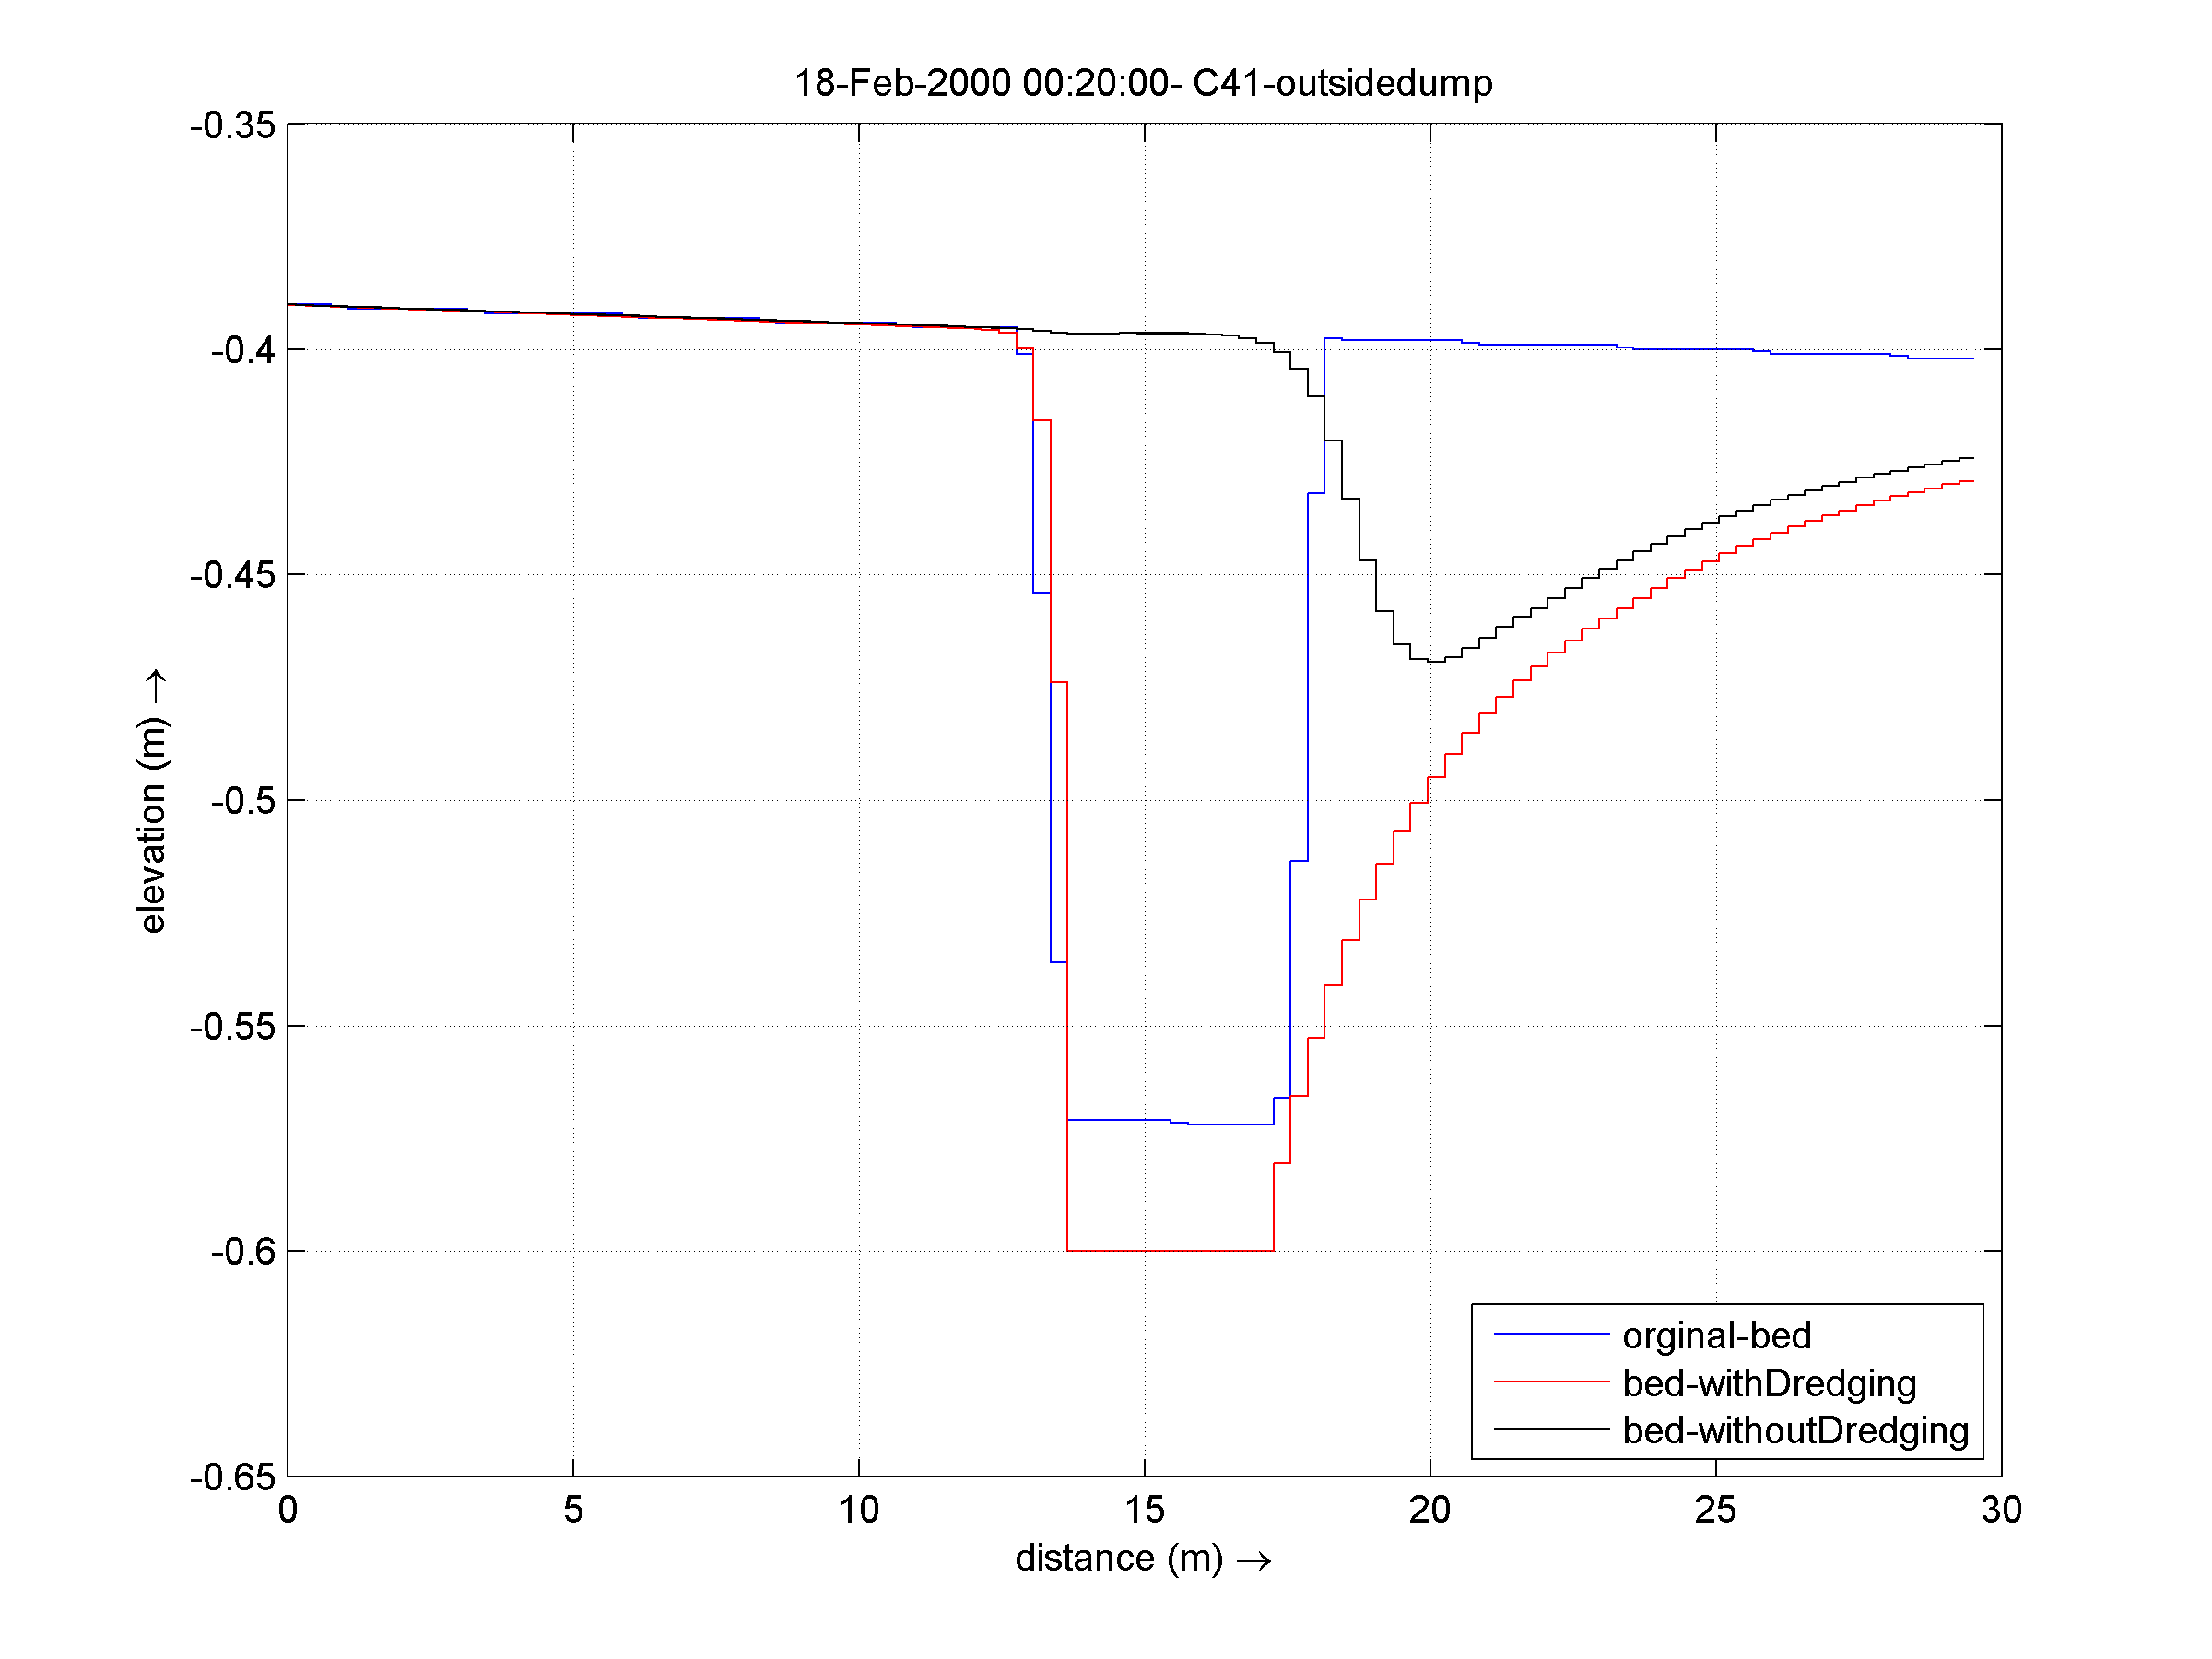
\includegraphics[width=0.7\columnwidth]{figures/C41-bedComparison-outsidedump.png}
	\end{center}\caption{c41- bed level at the centerline cross section of the model domain. blue line is the original bed level, the red line is the result of simulation with dredging and the black line is the result of simulation without dredging}
	\label{fig:C41-bedComparison-outsidedump}
\end{figure}

\begin{figure}[h!]
	\begin{center}
		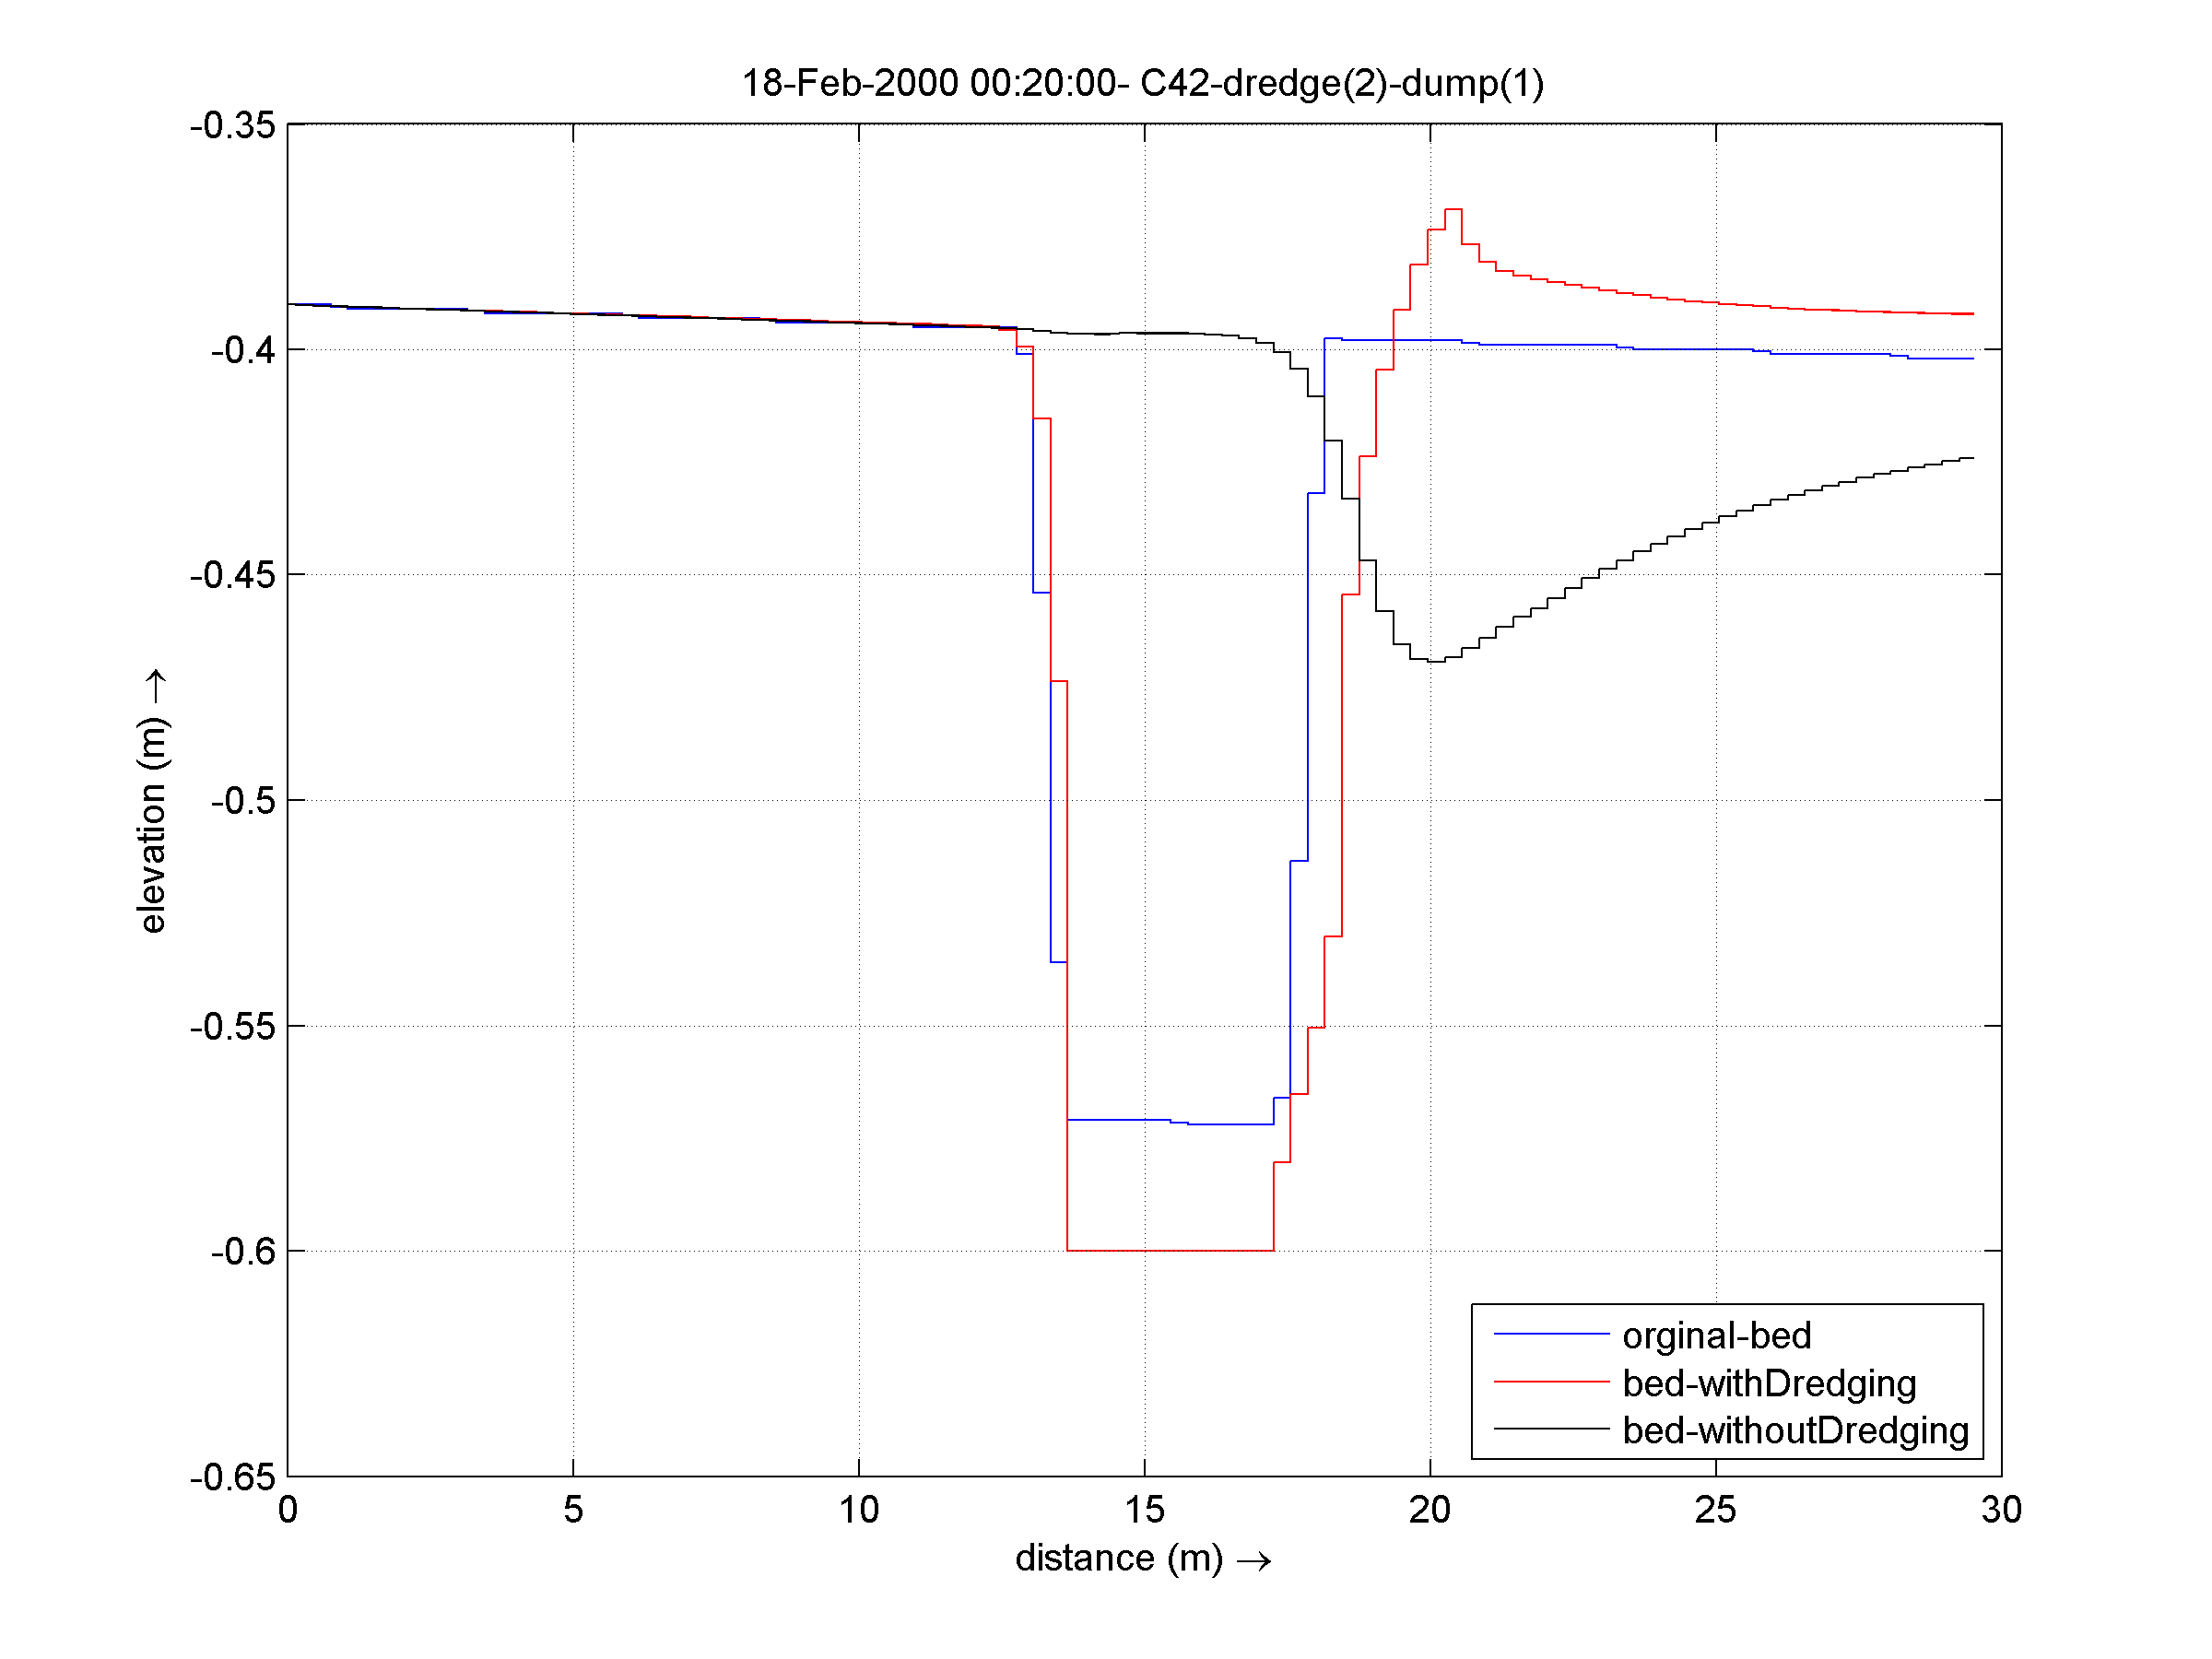
\includegraphics[width=0.7\columnwidth]{figures/C42-bedComparison-dredge2dump1.png}
	\end{center}\caption{c42- bed level at the centerline cross section of the model domain. blue line is the original bed level, the red line is the result of simulation with dredging and the black line is the result of simulation without dredging}
	\label{fig:C42-bedComparison-dredge2dump1}
\end{figure}

\begin{figure}[h!]
	\begin{center}
		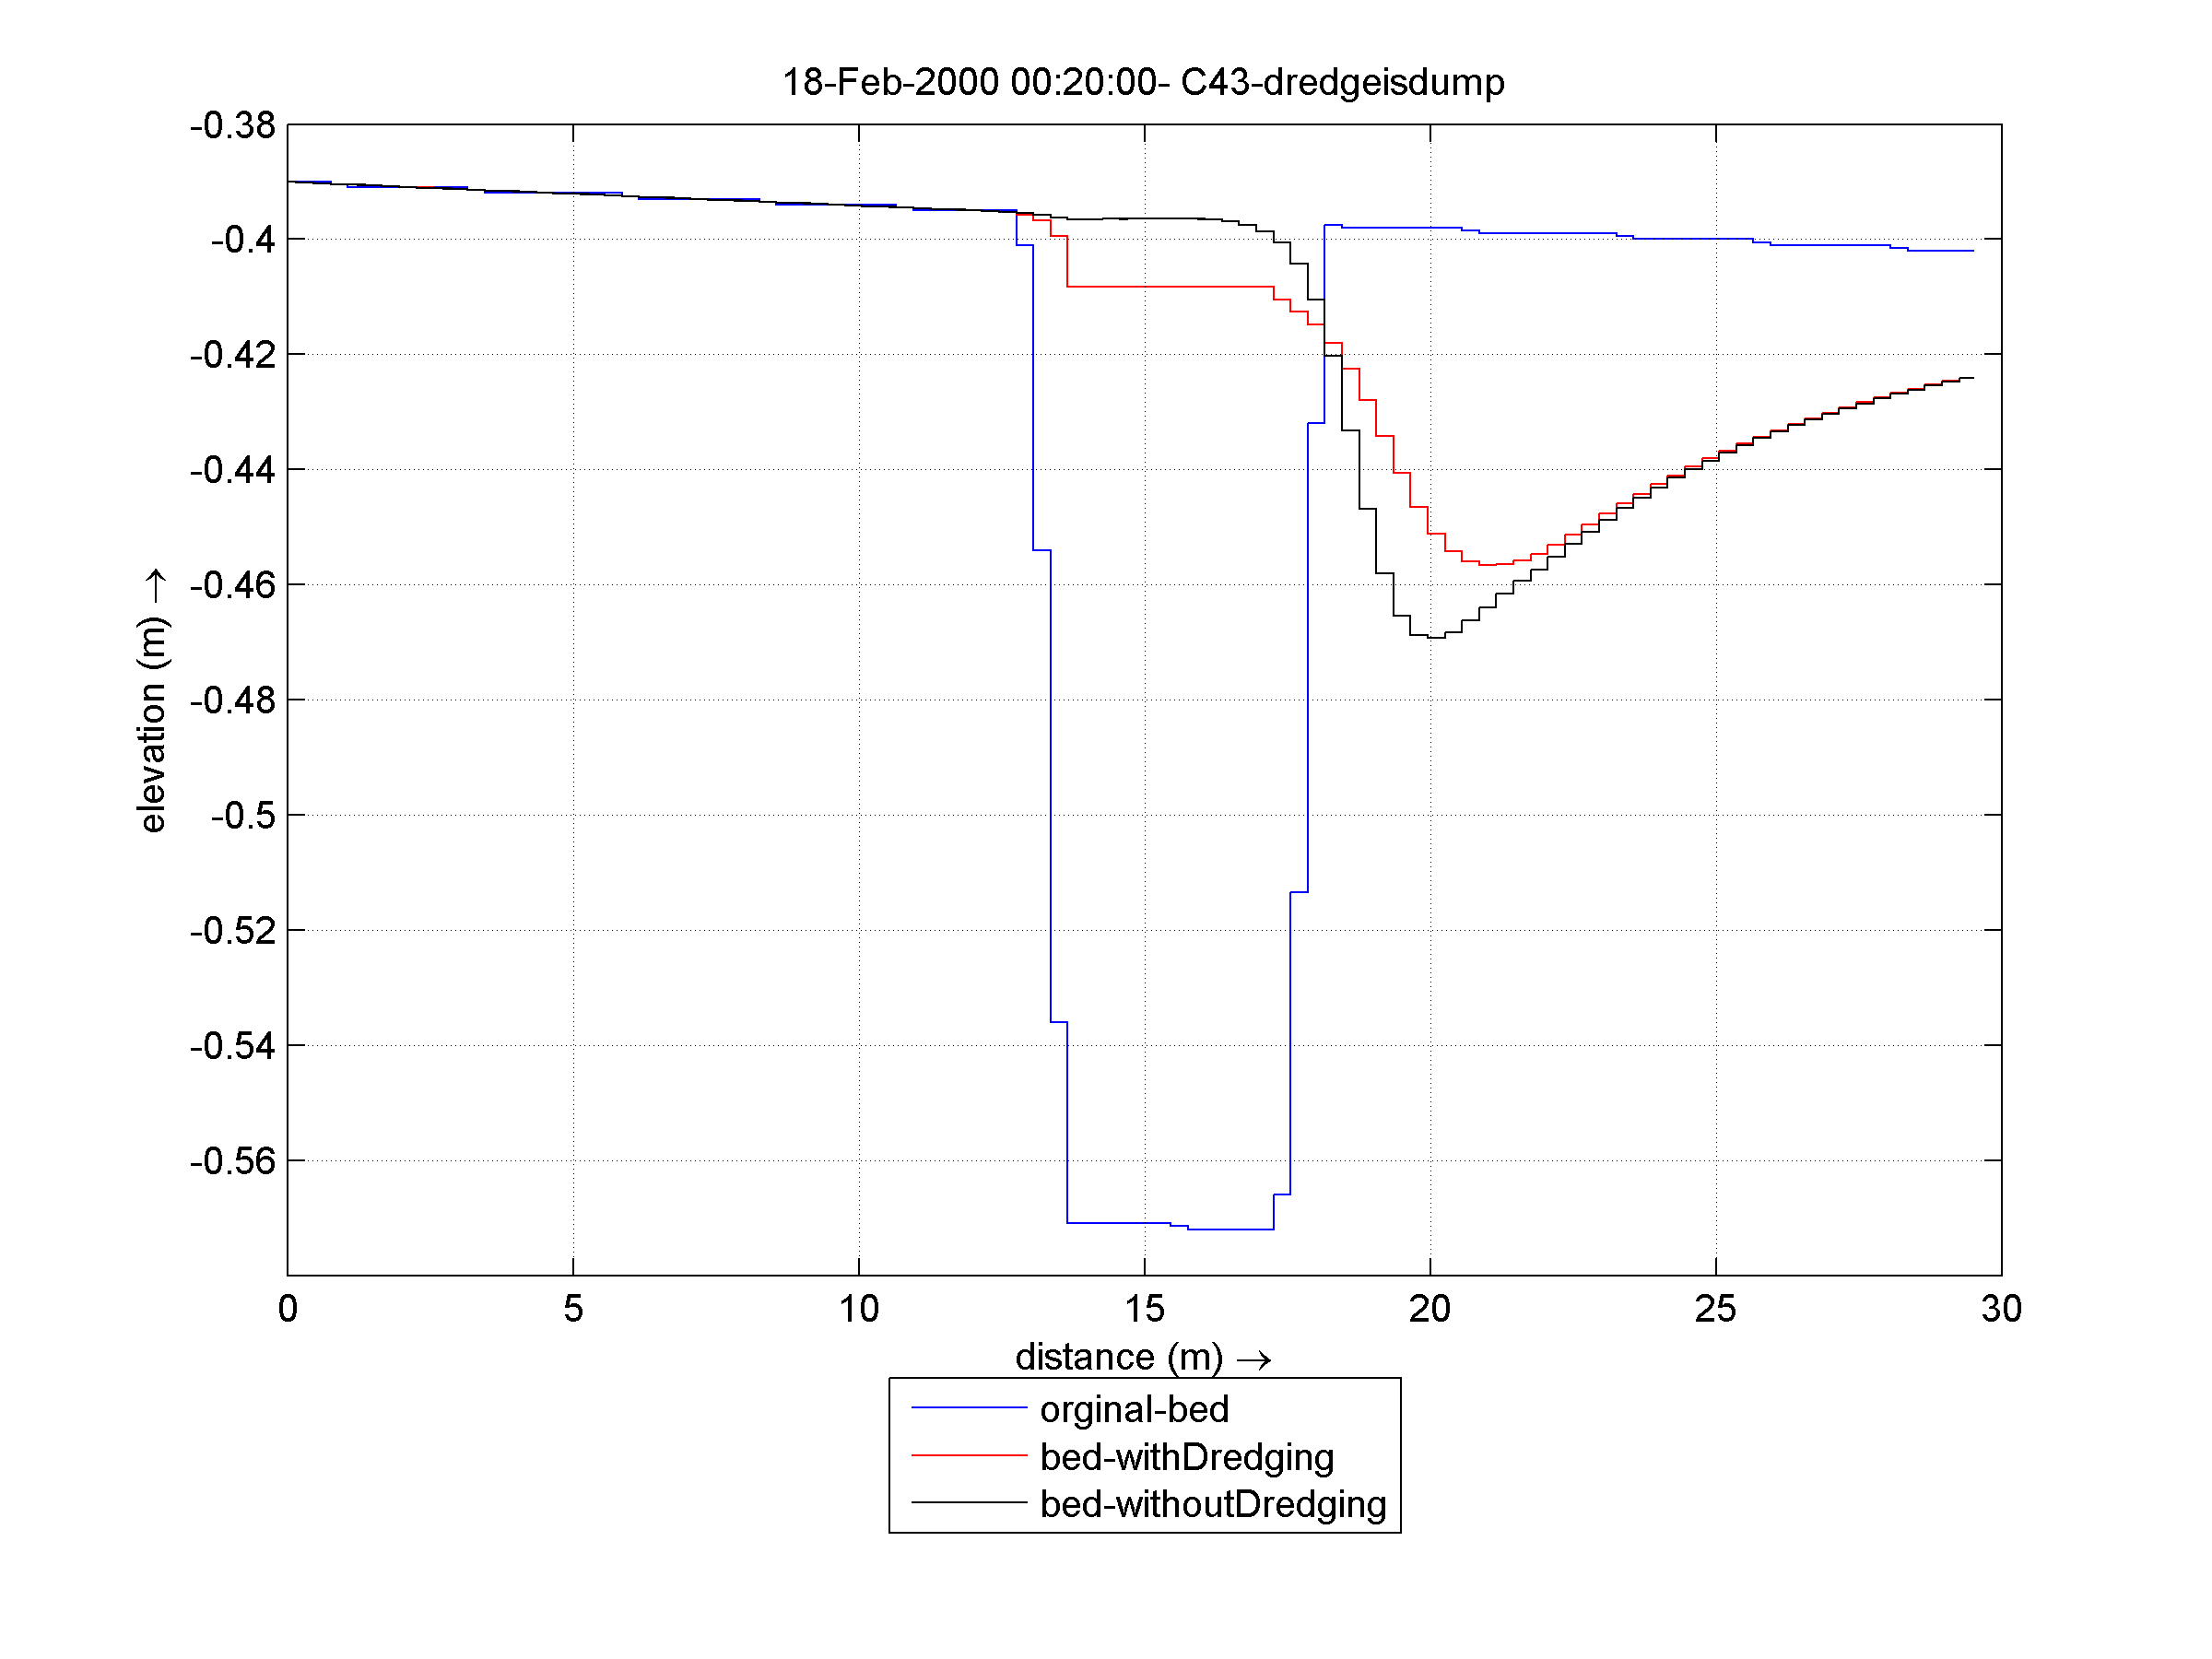
\includegraphics[width=0.7\columnwidth]{figures/C43-bedComparison-dredgeisdump.png}
	\end{center}
	\caption{c43- bed level at the centerline cross section of the model domain. blue line is the original bed level, the red line is the result of simulation with dredging and the black line is the result of simulation without dredging}
	\label{fig:C43-bedComparison-dredgeisdump}
\end{figure}

\begin{figure}[h!]
	\begin{center}
		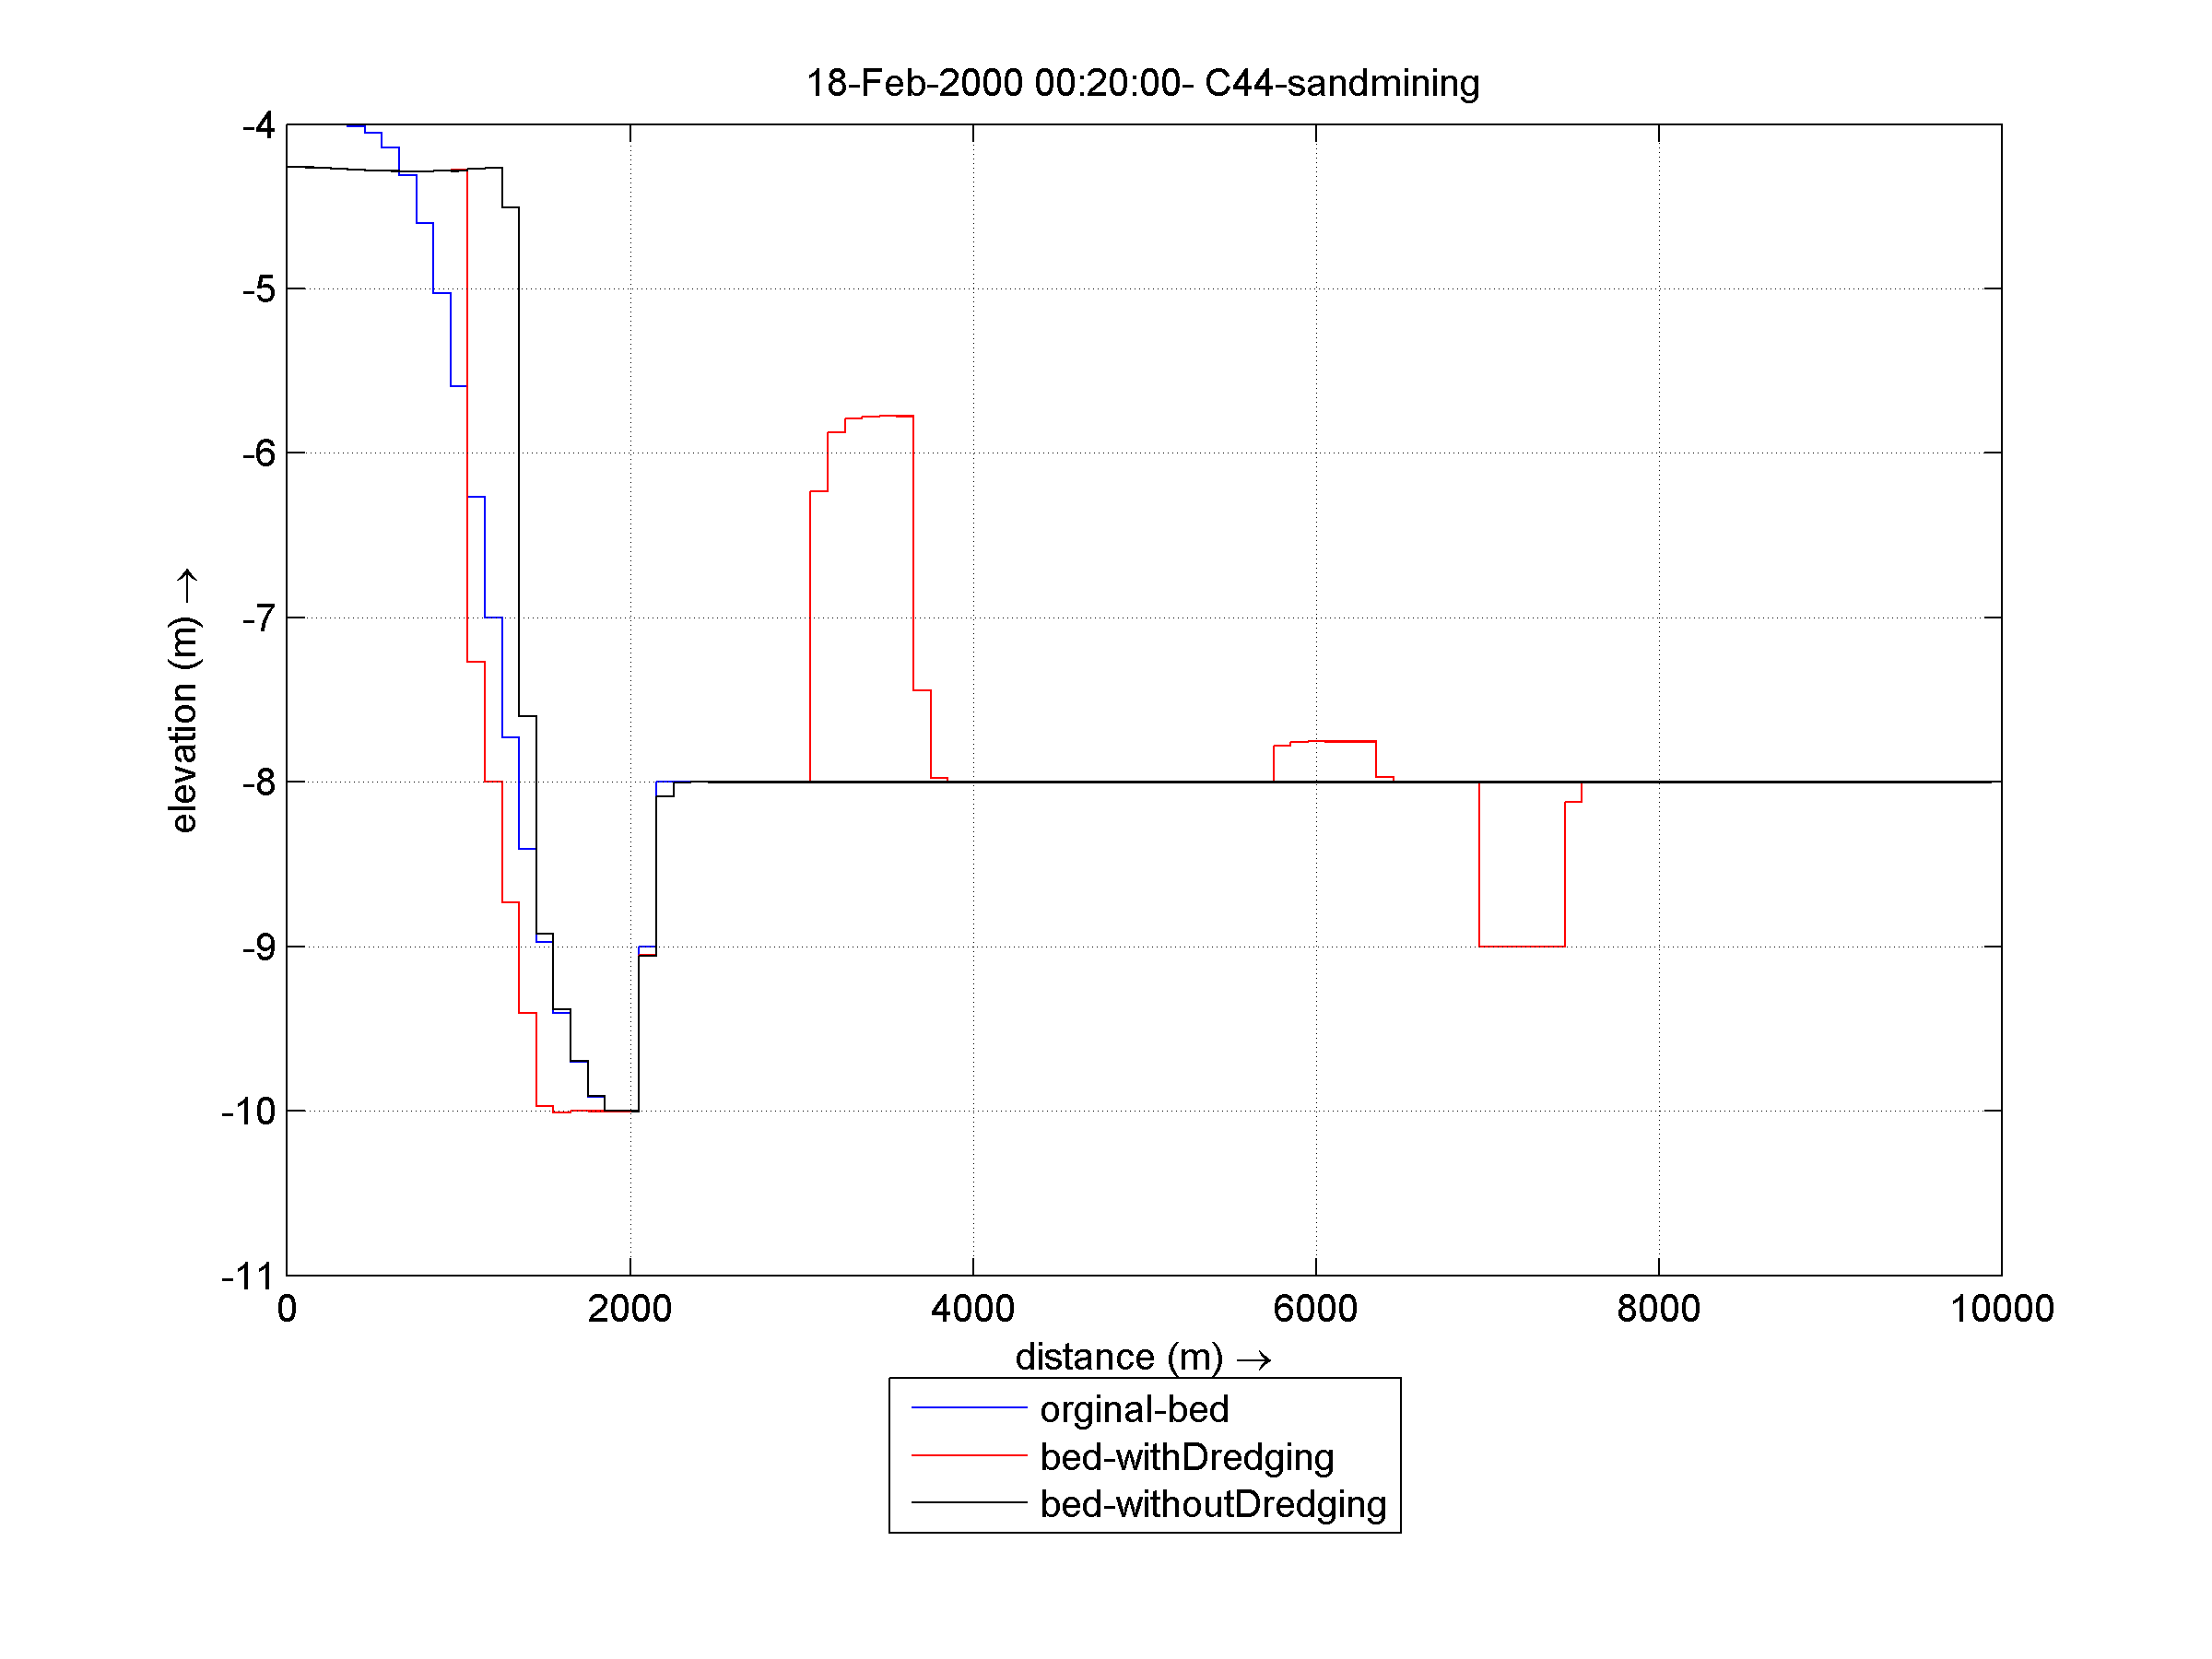
\includegraphics[width=0.7\columnwidth]{figures/C44-bedComparison-sandmining.png}
	\end{center}\caption{c44- bed level at the centerline cross section of the model domain. blue line is the original bed level, the red line is the result of simulation with dredging and the black line is the result of simulation without dredging}
	\label{fig:C44-bedComparison-sandmining}
\end{figure}
\paragraph*{C45 test-case with one mixed layer (unstructured grid)}
In this test-case, we convert the structured grid used in c35 case to unstructured grid (see figure \ref{fig:C45Unstructuredgrid}). The same boundaries, models parameters and dredging-dumping conditions of c35 are applied to c45. 

\begin{figure}[h!]
	\begin{center}
		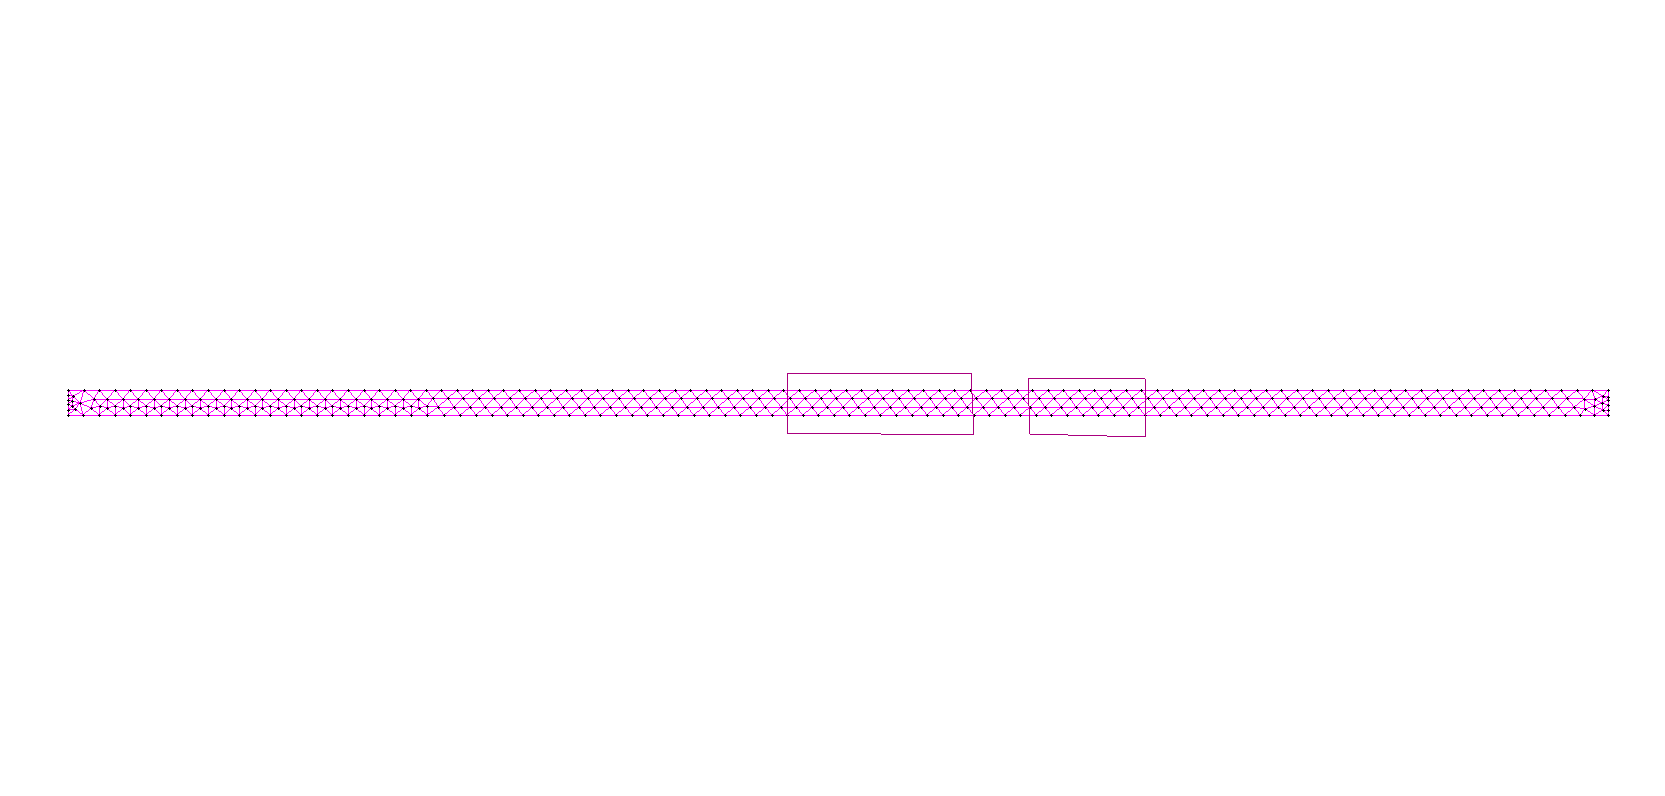
\includegraphics[width=0.7\columnwidth]{figures/C45Unstructuredgrid.PNG}
	\end{center}\caption{c45- Unstructured grid used}
	\label{fig:C45Unstructuredgrid}
\end{figure}
The bed change at the centerline of c45 is compared to the similar bed change longitudinal section of c35 as shown in figure \ref{fig:C45triangles-bedComparison}. The result shows that both bed change behavior of structured and unstructured grid is similar

\begin{figure}[h!]
	\begin{center}
		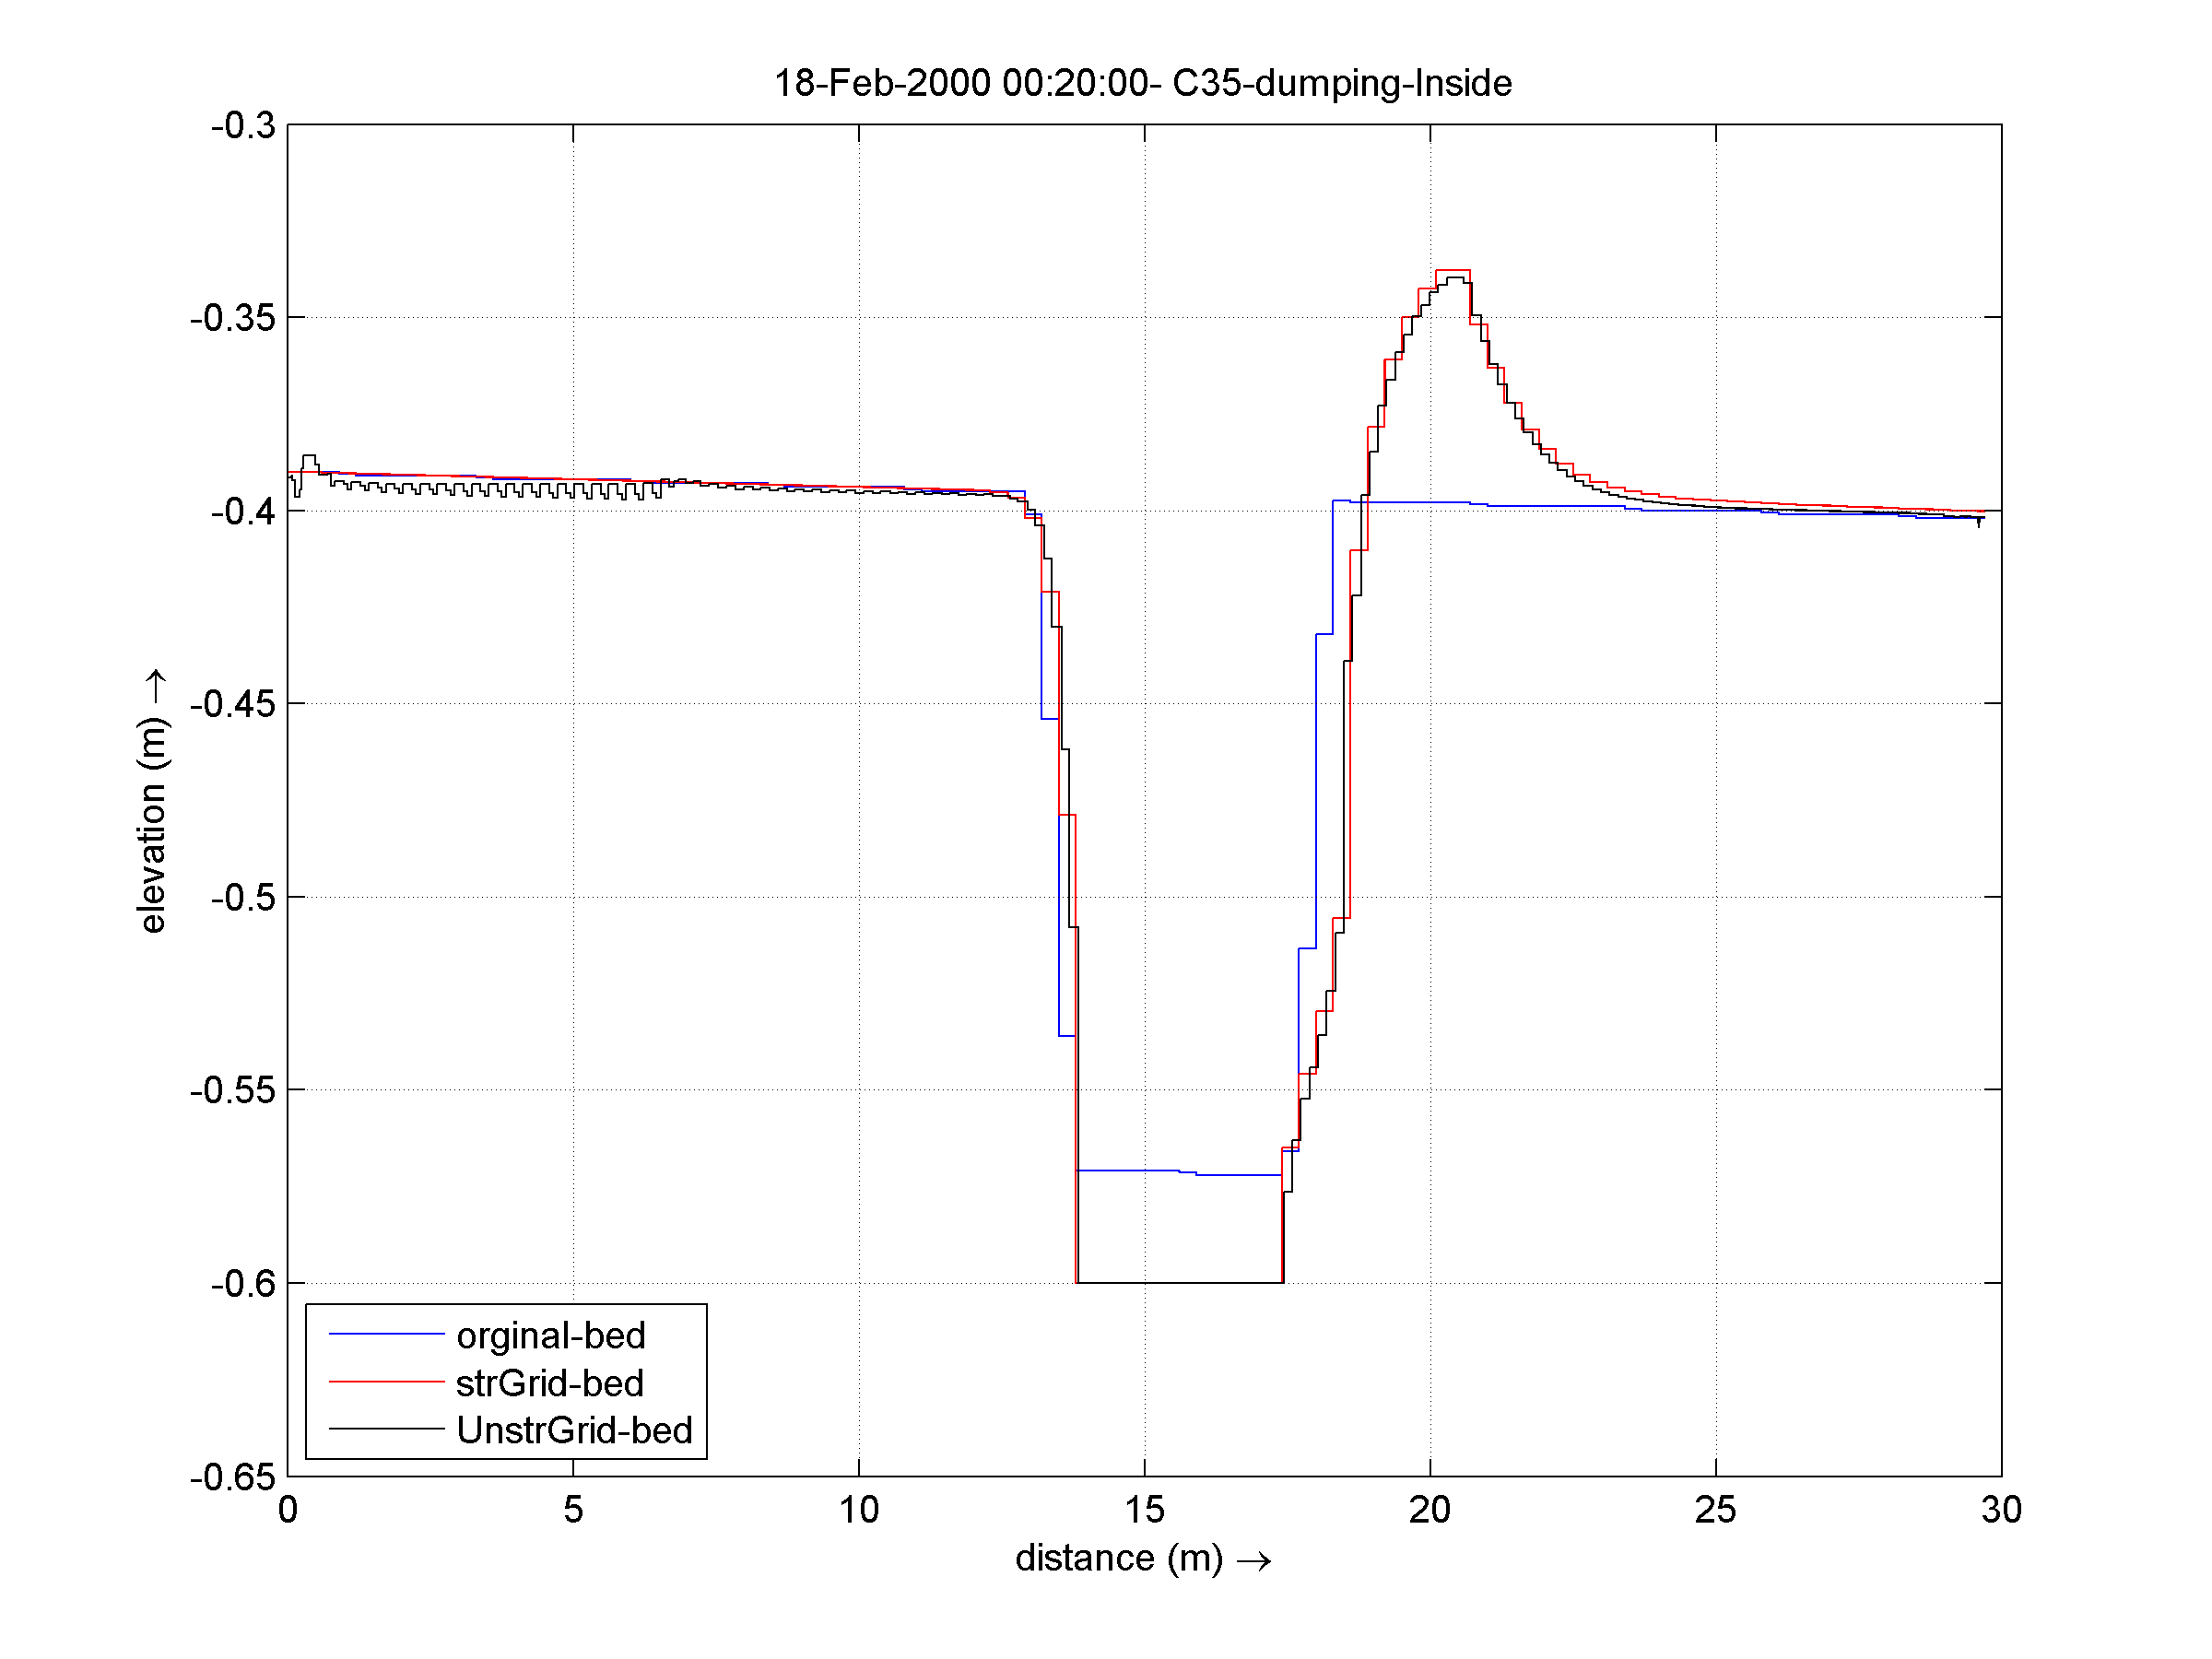
\includegraphics[width=0.7\columnwidth]{figures/C45triangles-bedComparison.png}
	\end{center}\caption{A comparison between bed level change at the model longitudinal centerline of c45 (unstructured grid - UnstrGrid) and c35 (structured grid - strGrid)}
	\label{fig:C45triangles-bedComparison}
\end{figure}

\subparagraph*{c46 nourishment}
This test case is created to test the nourishment function in FM (Sed-mor). The same model setup and parameters used in c35 is applied to c46. However, instead of dredging sediment nourishment is imposed to the model. A similar Delft3D4 model is also setup to compare the result of both model. The sediment in this test cae is dumped in two location as shown in figure \ref{fig:C46Net1} . The spinup time to start the morphological computation on the mor file is set to 5 minutes. The data file used is illustrated below:

\begin{verbatim}
[DredgeFileInformation]
FileCreatedBy      	 = WL | DH, Delft3D-QUICKIN Version 4.11.00; Feb 2004
FileCreationDate 		 = 15:32:06, 05-03-2004
FileVersion   			 = 01.02   
PolygonFile    		 = nourishment.pol
DredgeWhileMorfac0 	 = true
[Nourishment]
Name        			 = NOR
Volume   			     = 0.20
DistrOverDump			 = 1
Dump 					 = Nor
Percentage				 = 100
[Nourishment]
Name       		     = KUIL
Volume    			     = 0.50
DistrOverDump			 = 1
Dump 					 = KUIL
Percentage				 = 100

\end{verbatim}

\begin{figure}[h!]
	\begin{center}
		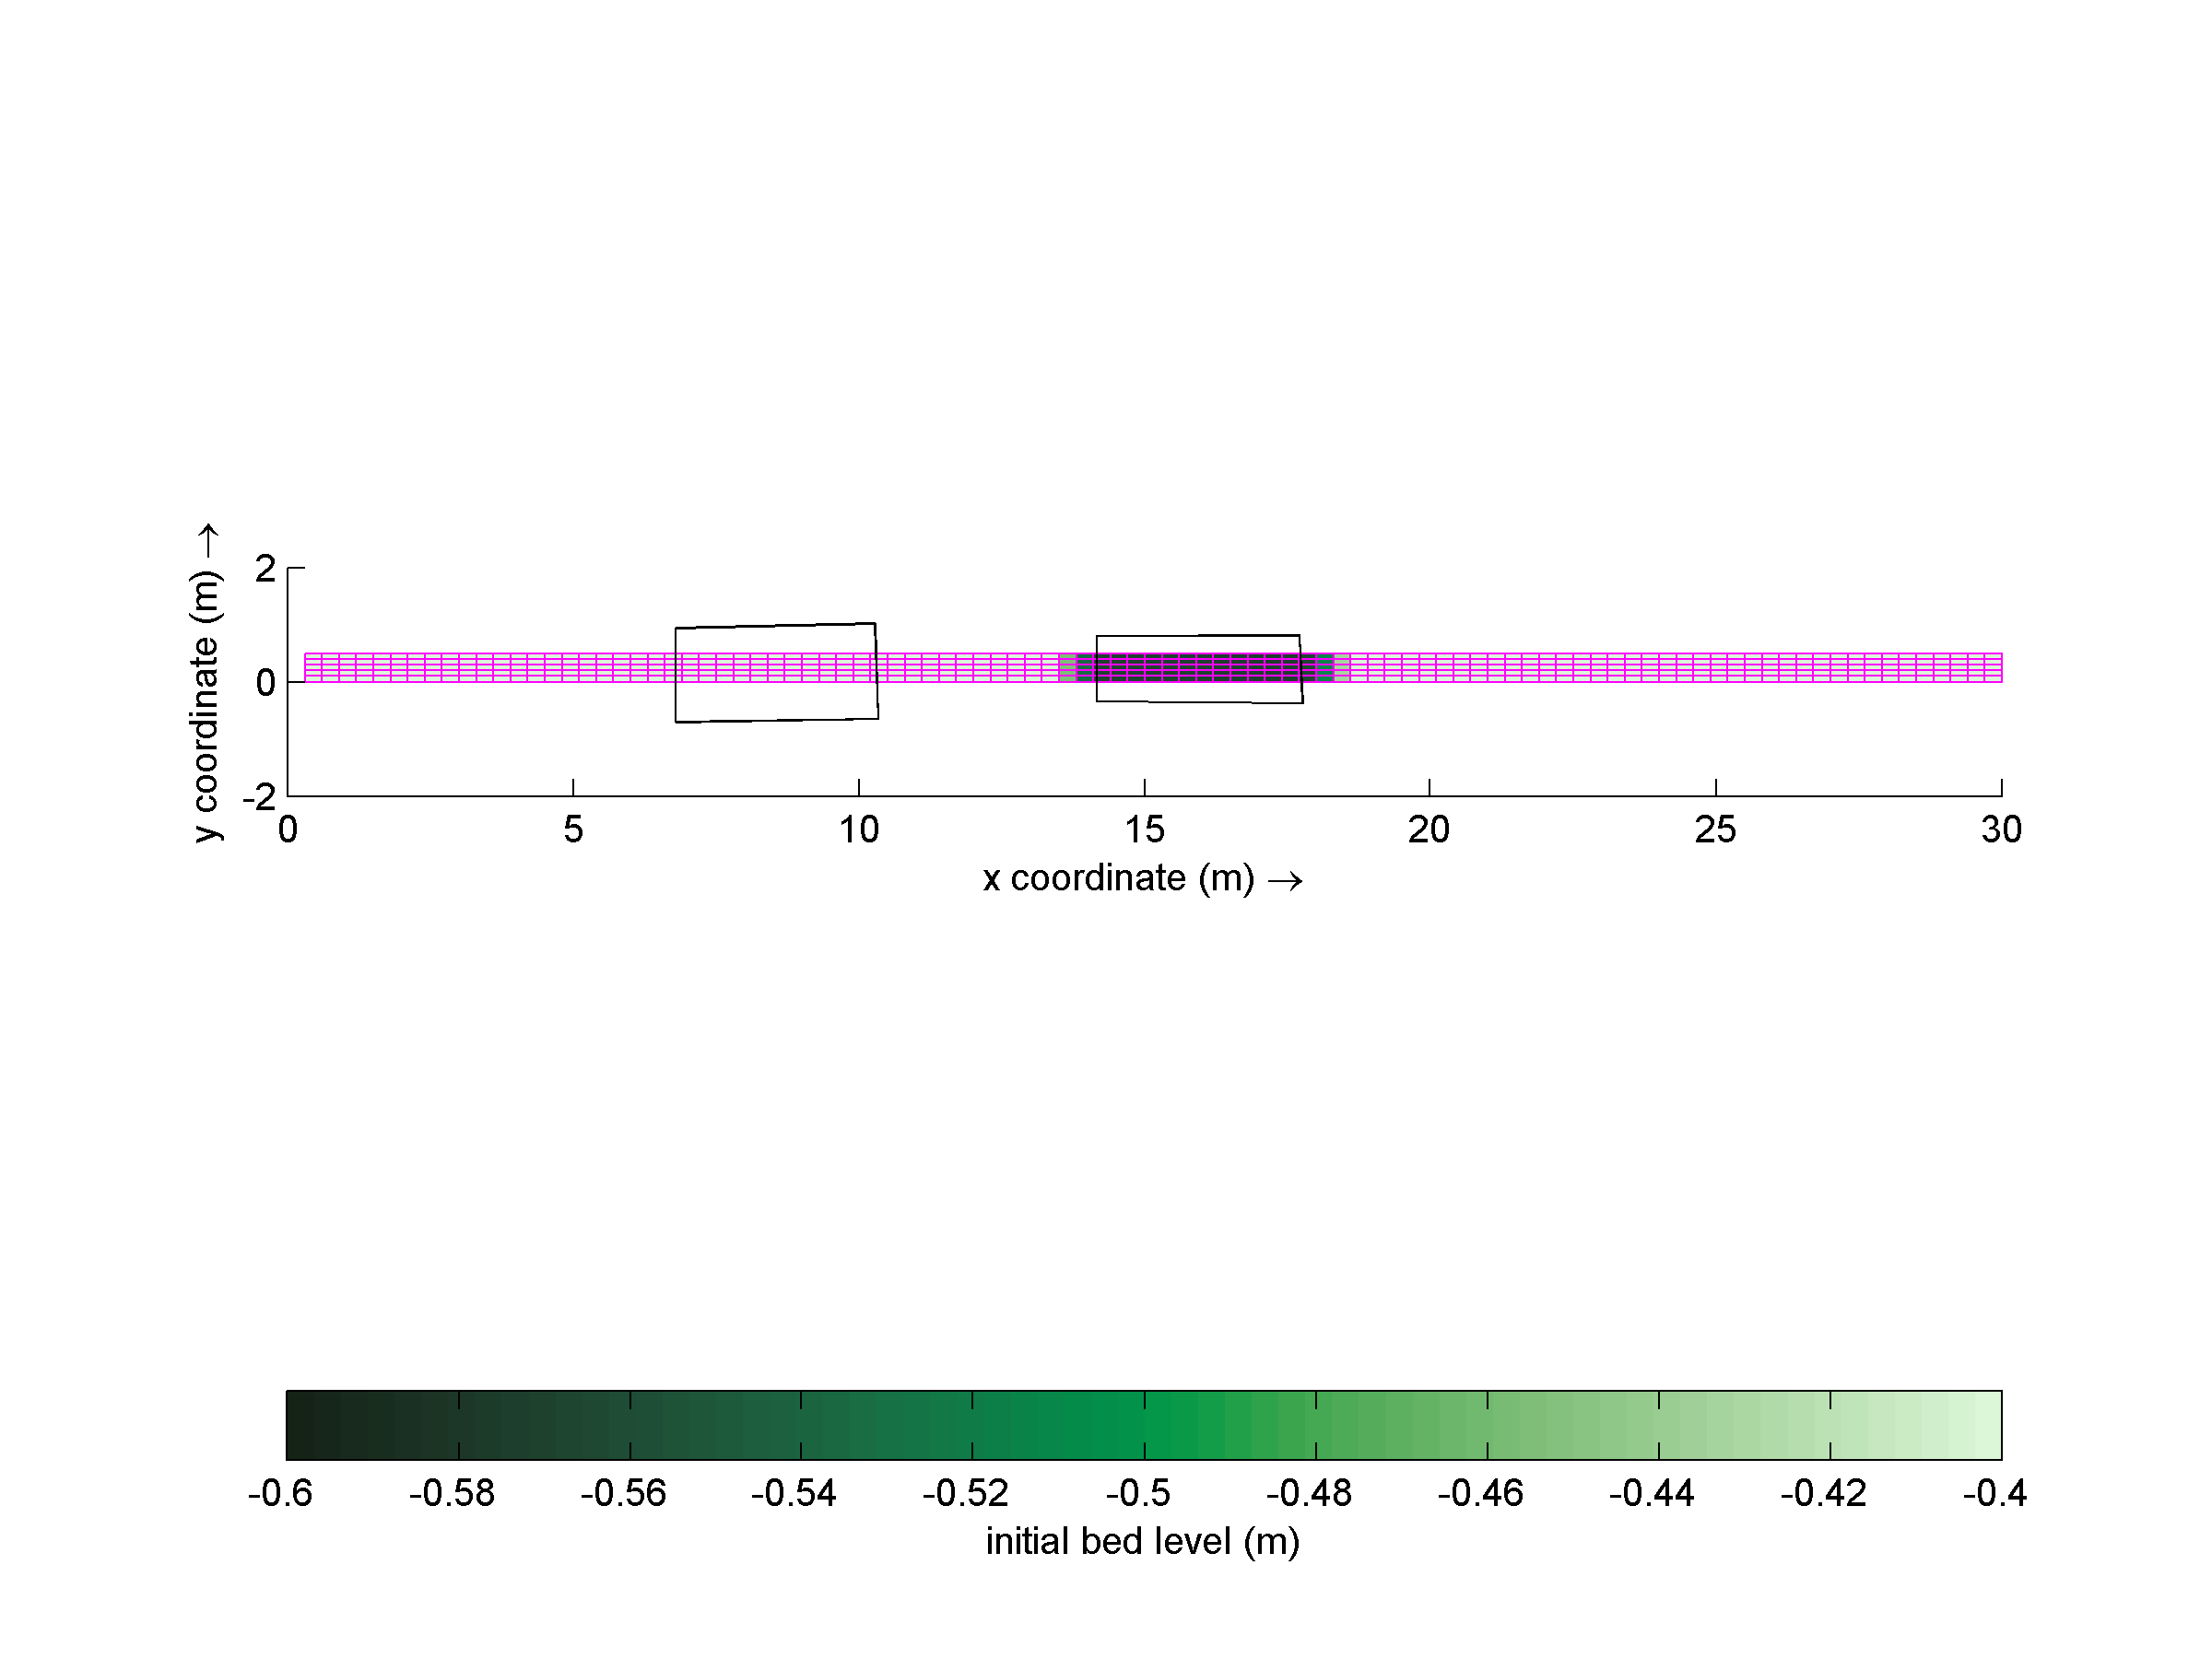
\includegraphics[width=0.7\columnwidth]{figures/C46Net1.png}
	\end{center}\caption{The Grid used and depth used in the model. The figure also shows the locations of sediment nourishment bounded with polygons}
	\label{fig:C46Net1}
\end{figure}
The result comparison illustrates that the FM produce similar behavior as Delft3D4. However, the start time of dumping sediment to the model in FM is exactly after the spin-up time (5 minutes), while in Delft3D after the first time step (0.03 min) after the spin up time at 5.03 minutes (see figure \ref{fig:test}).

\begin{figure}
	\centering
	\begin{subfigure}{.5\textwidth}
		\centering
		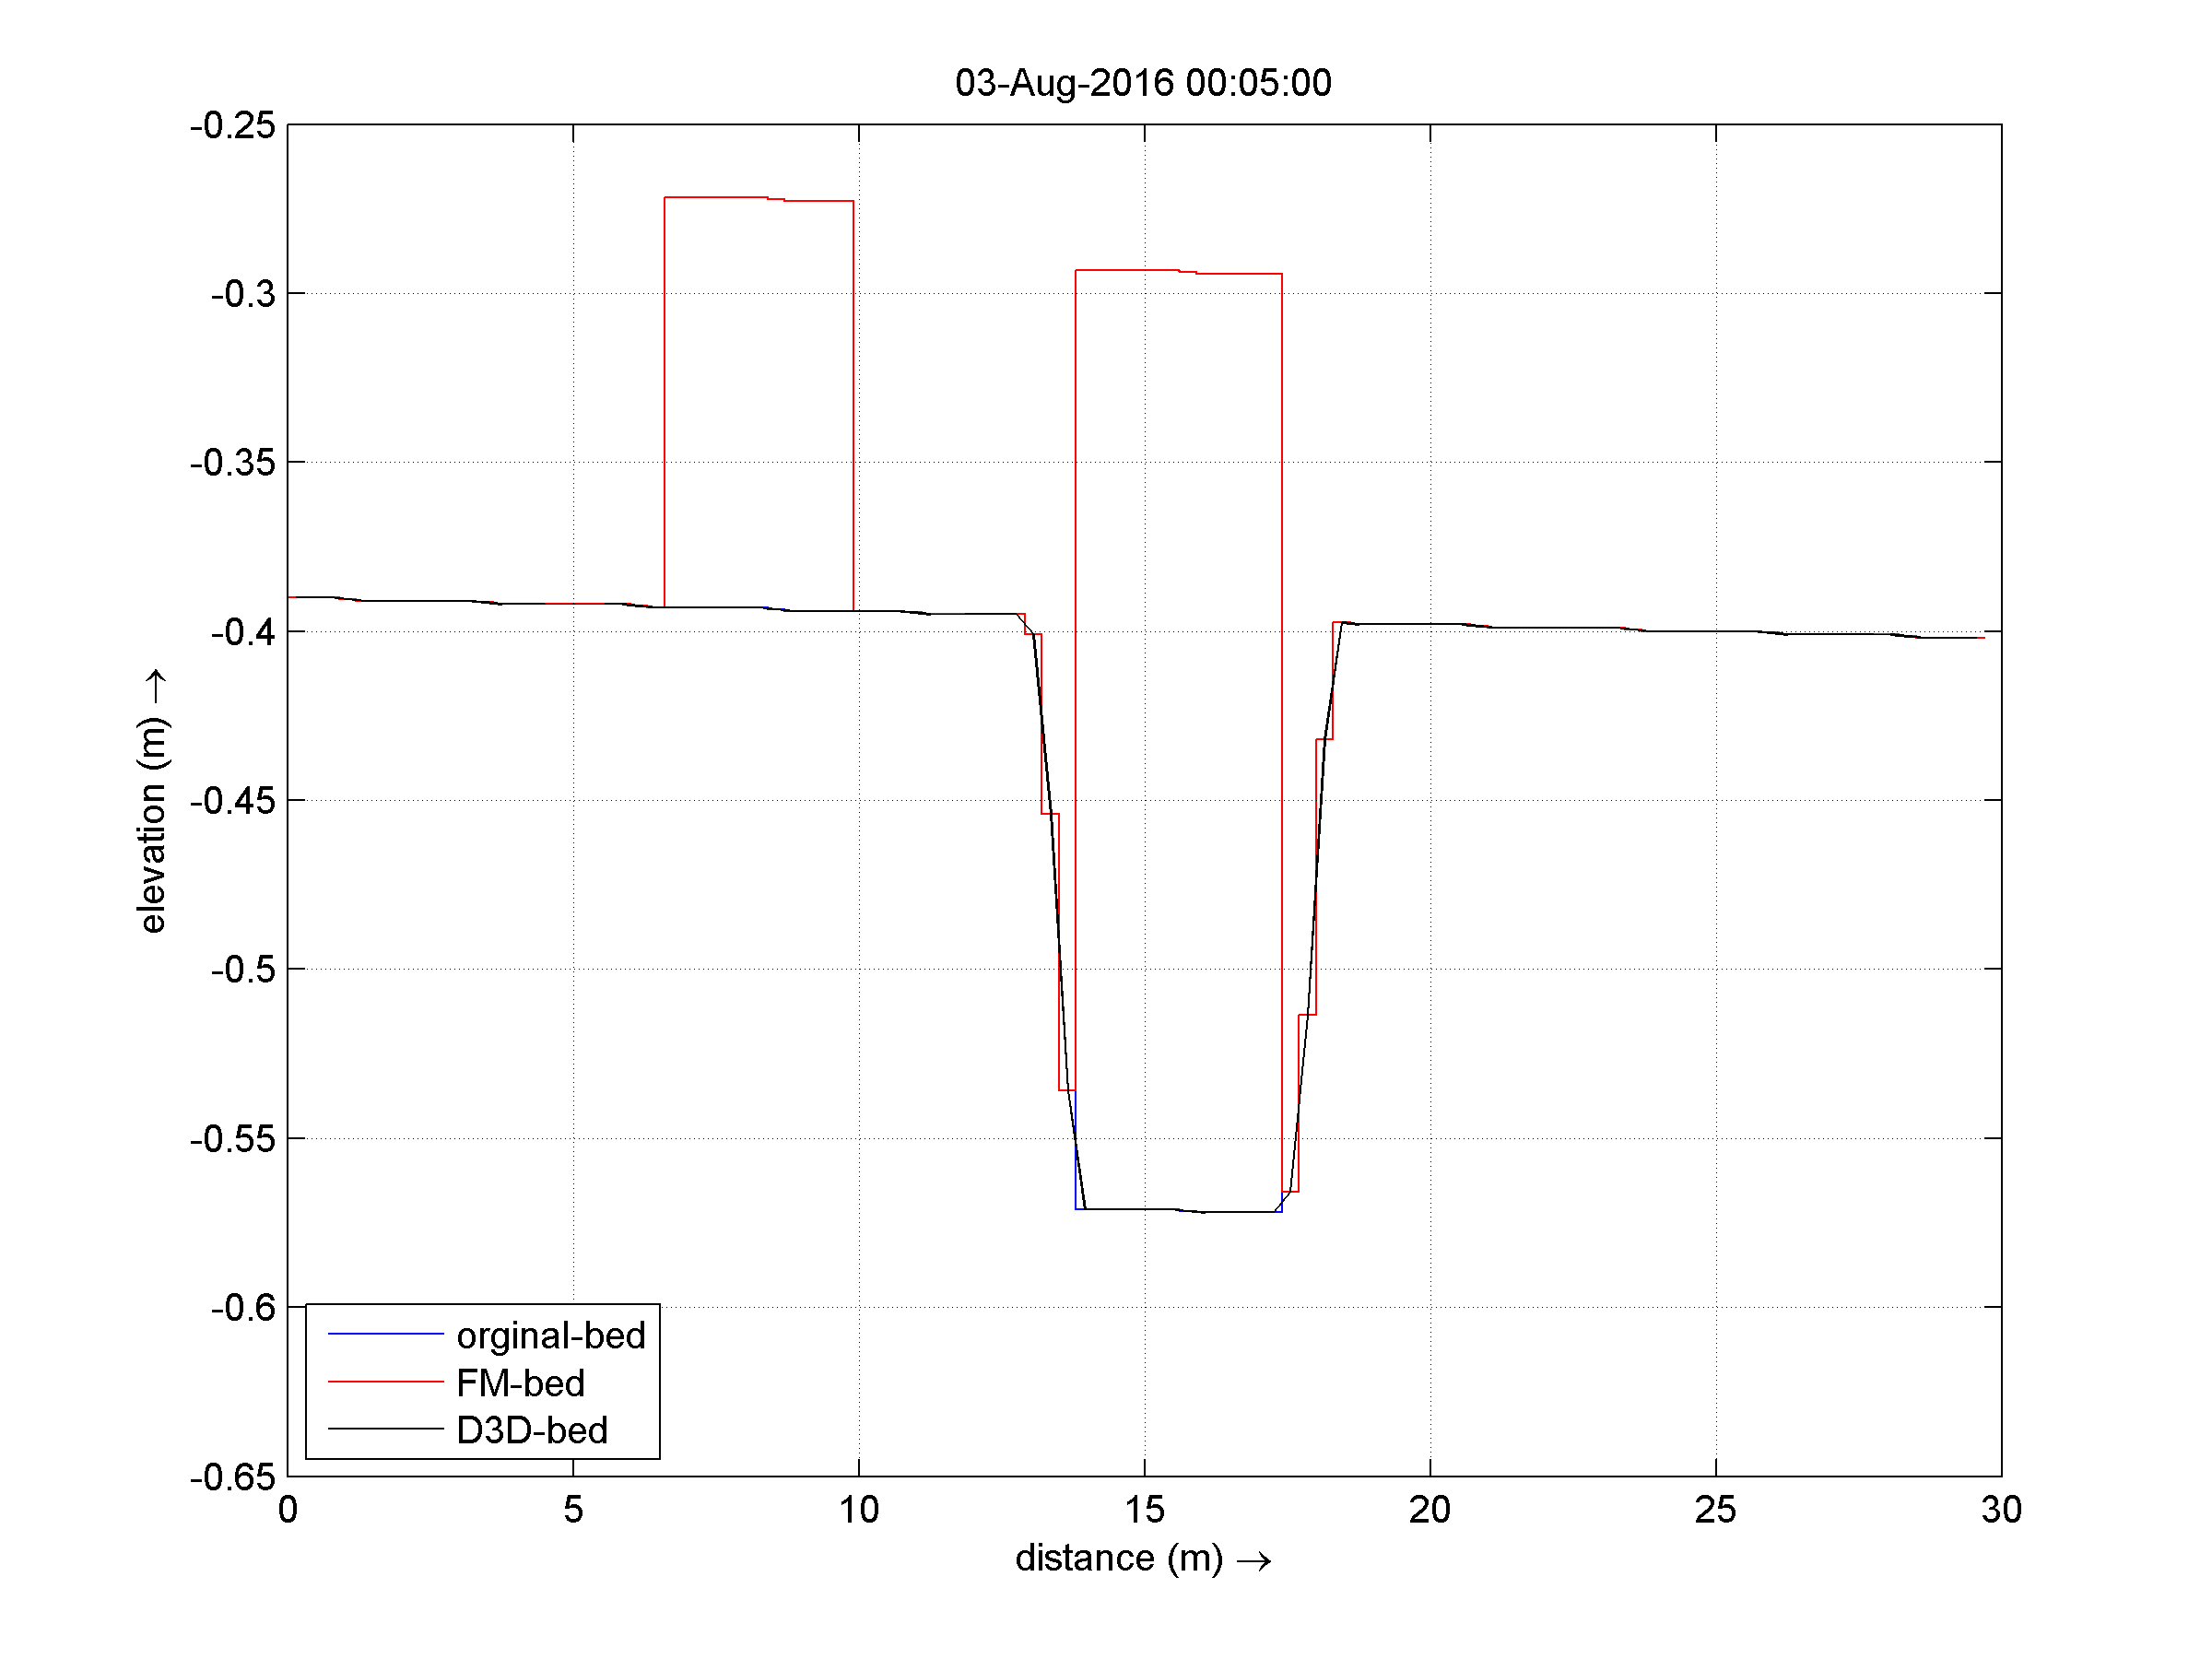
\includegraphics[width=.9\linewidth]{figures/C46result101.png}
		\caption{The result of the bed change after 5 minutes}
		\label{fig:sub1}
	\end{subfigure}%
	\begin{subfigure}{.5\textwidth}
		\centering
		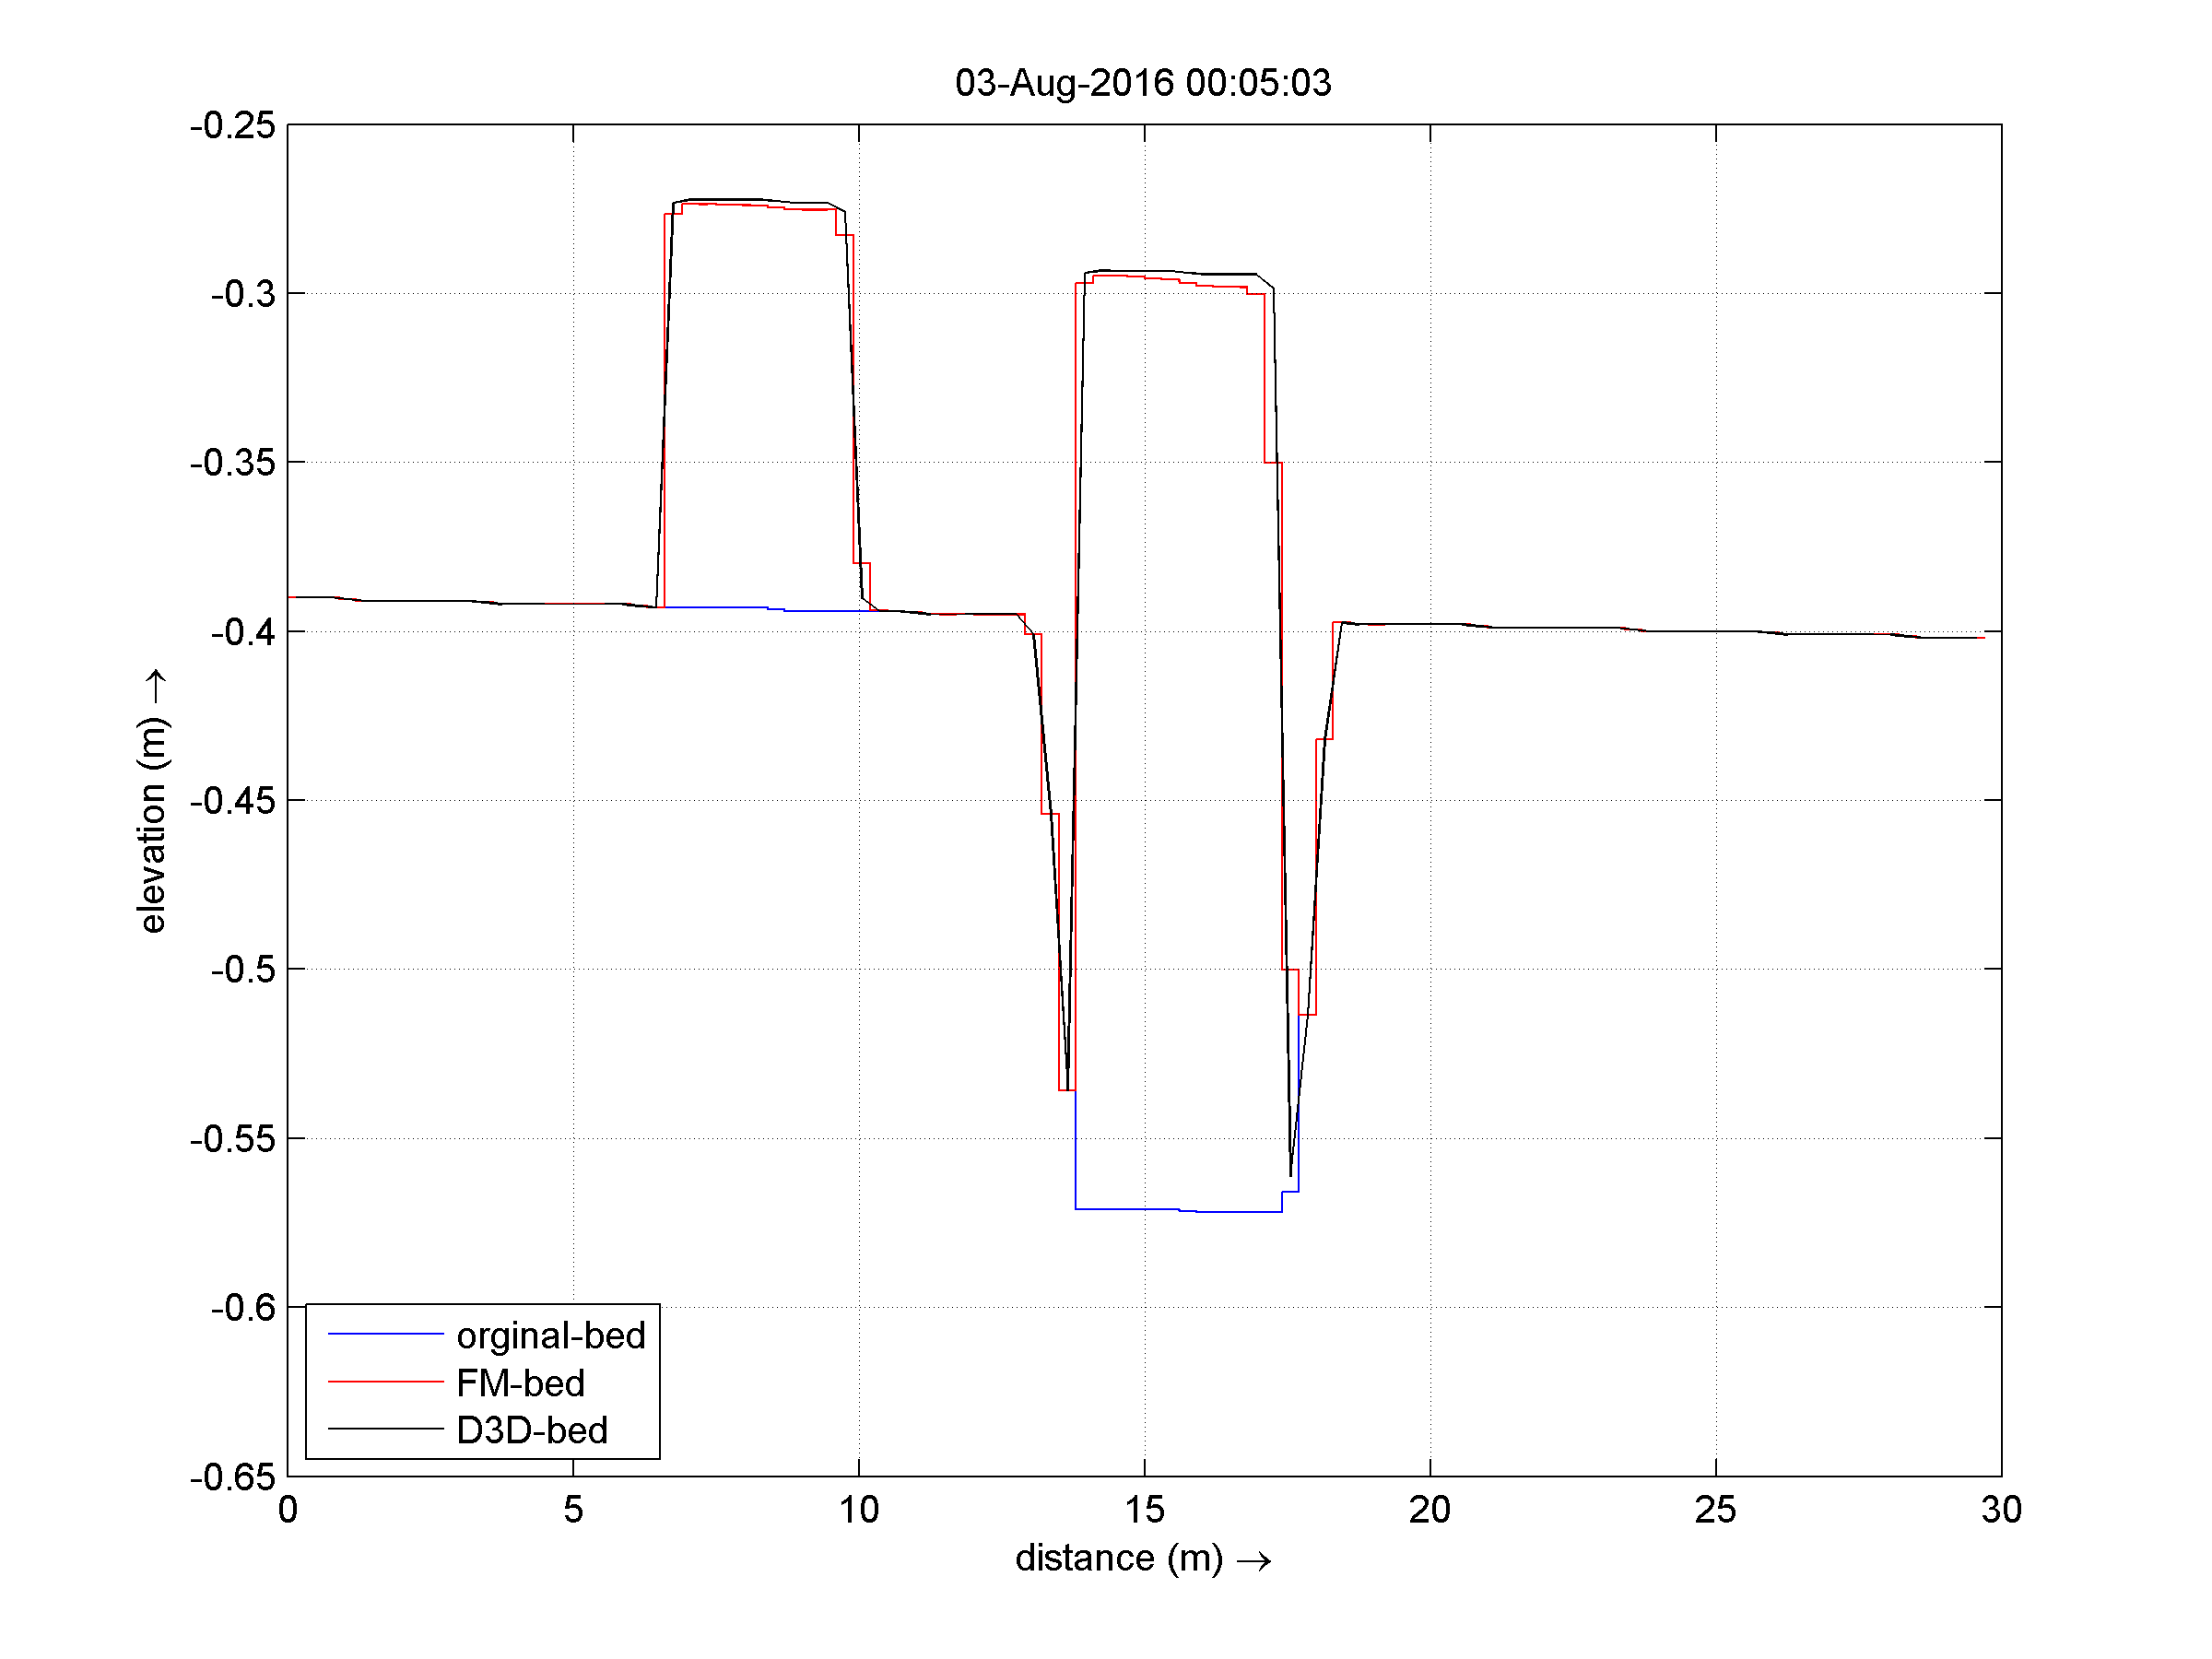
\includegraphics[width=.9\linewidth]{figures/C46result102.png}
		\caption{The result of the bed change after 5.03 minutes}
		\label{fig:sub2}
	\end{subfigure}
	\caption{ A comparison between FM and D3D: bed level change at the centerline of the channel (C46)}
	\label{fig:test}
\end{figure}

However, the final result of the bed change after 20 minutes of simulation running time shows small different in the magnitude of bet change as shown in figure \ref{fig:C4620min}. This might be due to slight difference in velocity bewtween both models (compare figure \ref{fig:C46V20min}).
\begin{figure}[h!]
	\begin{center}
		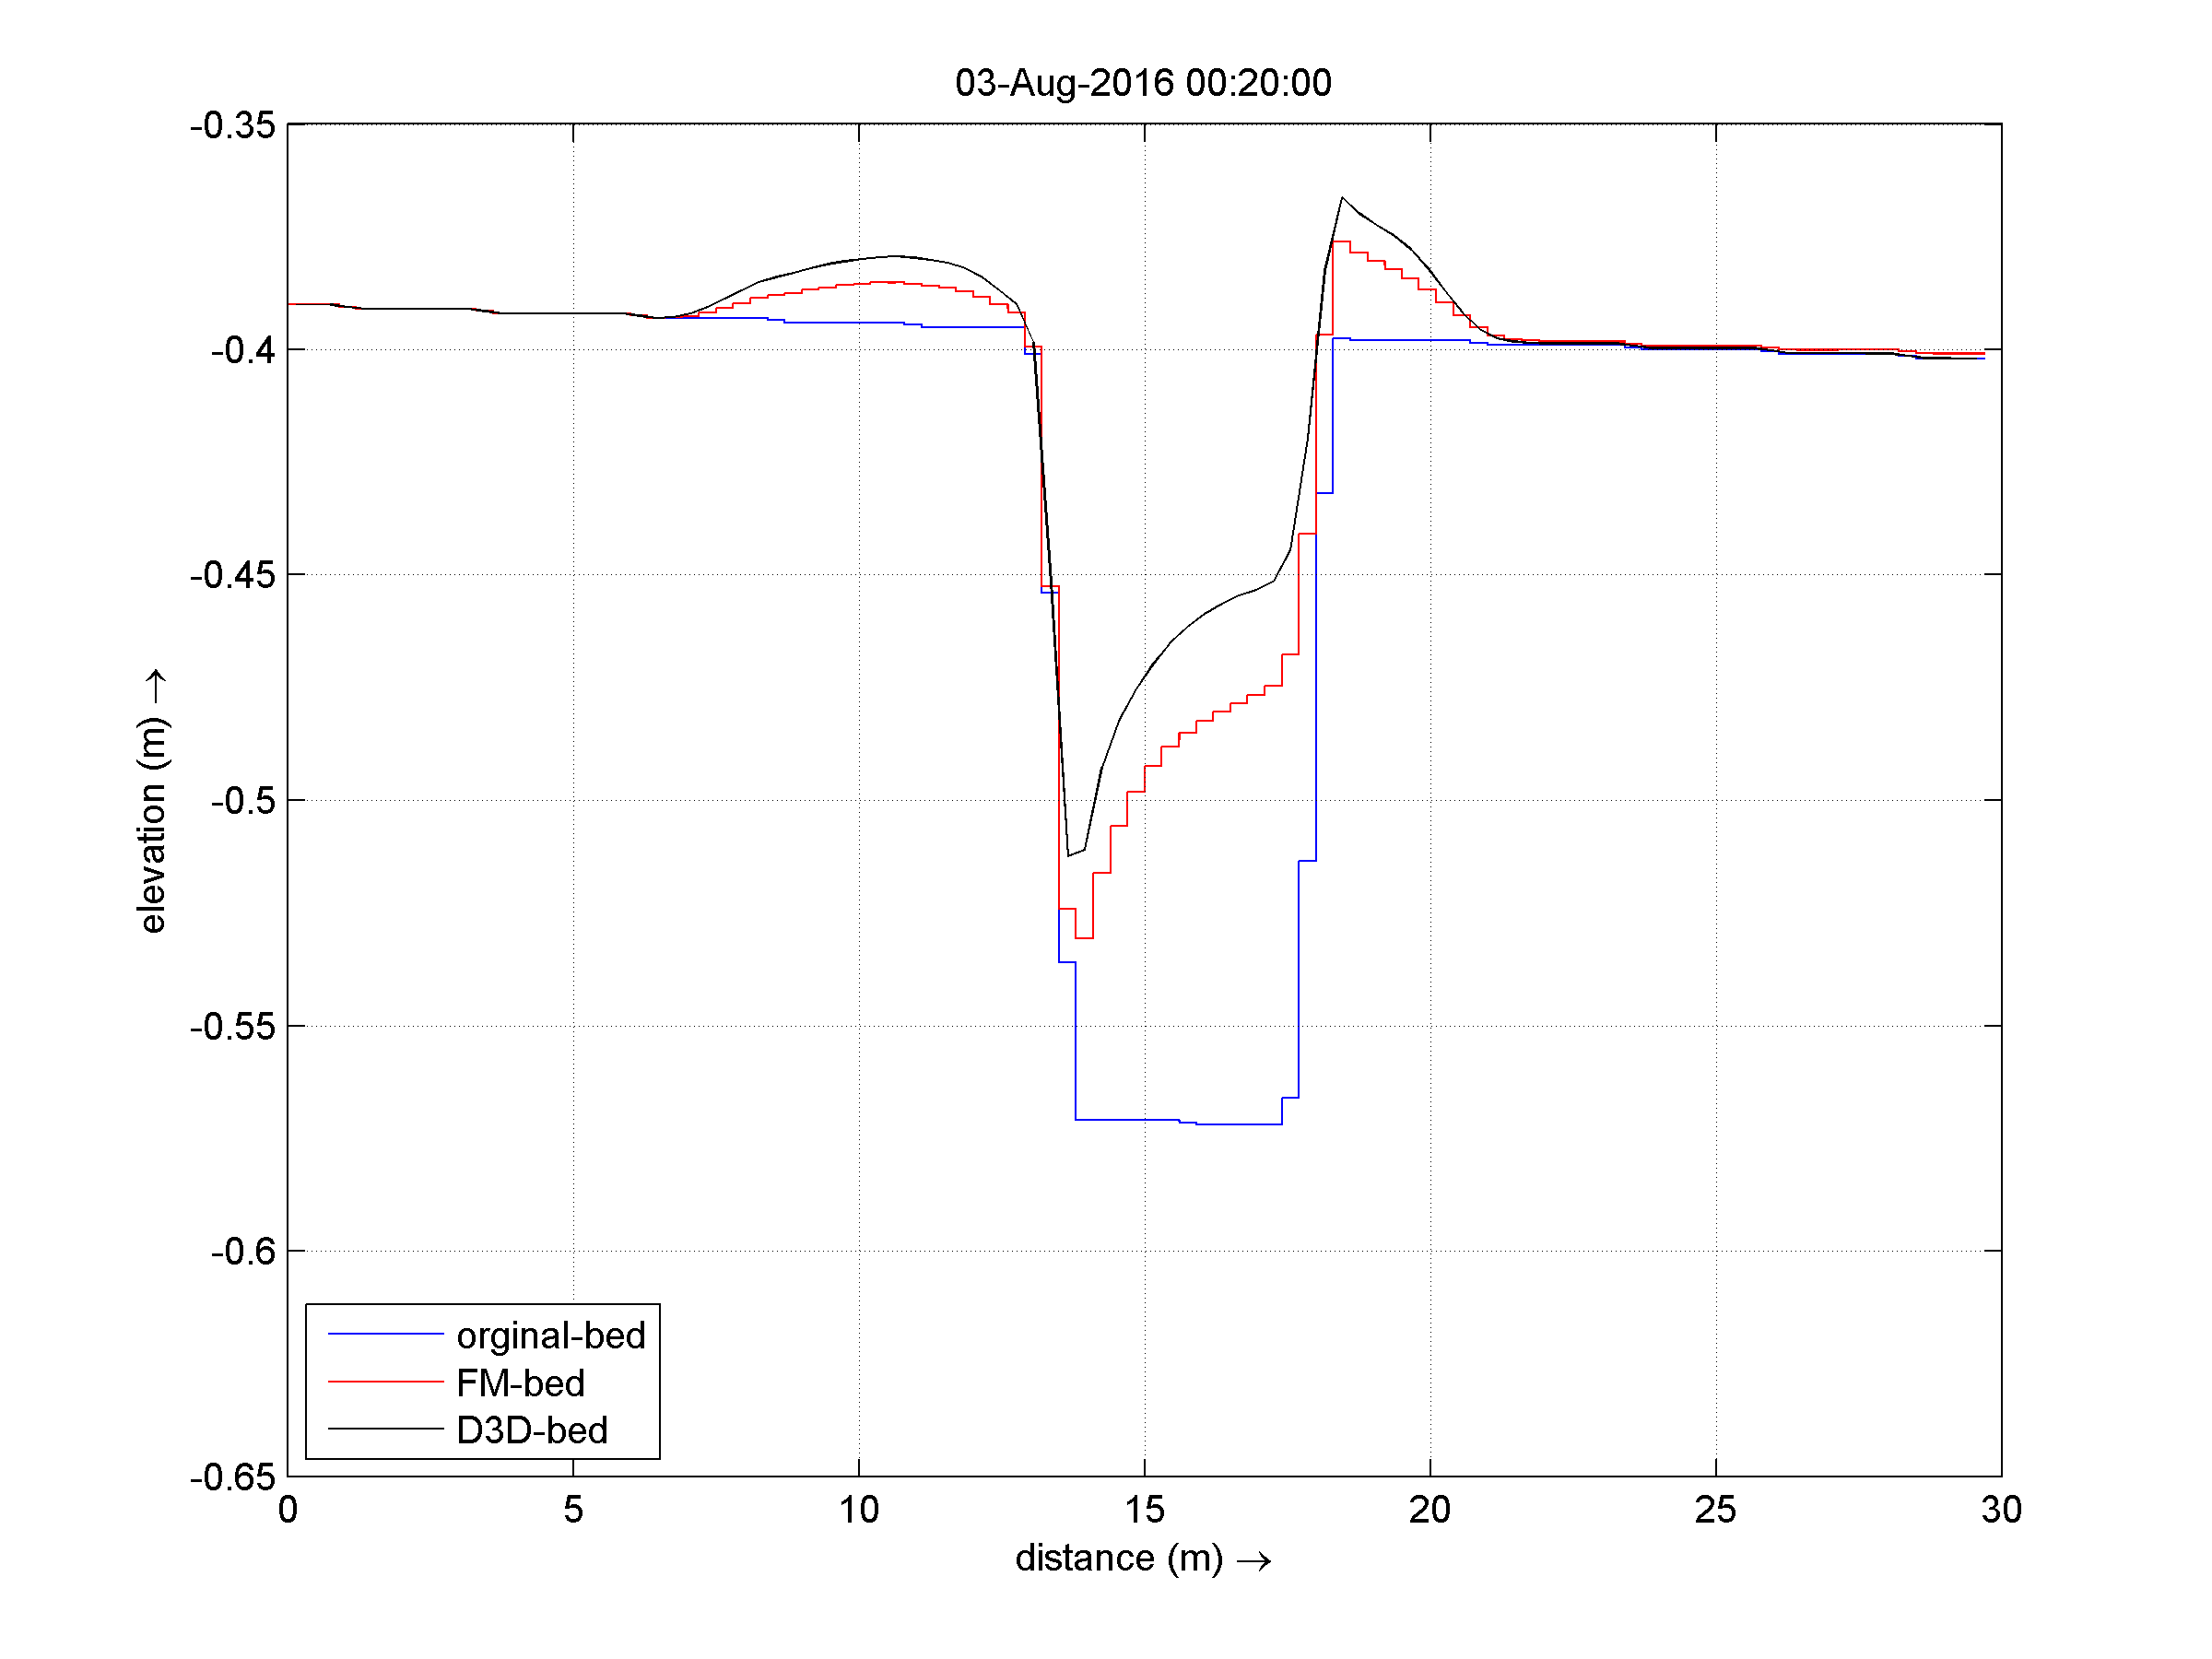
\includegraphics[width=0.7\columnwidth]{figures/C46result401.png}
	\end{center}\caption{A comparison between FM and D3D: bed level change at the centerline of the channel after 20 minutes (C46)}
	\label{fig:C4620min}
\end{figure}

\begin{figure}[h!]
	\begin{center}
		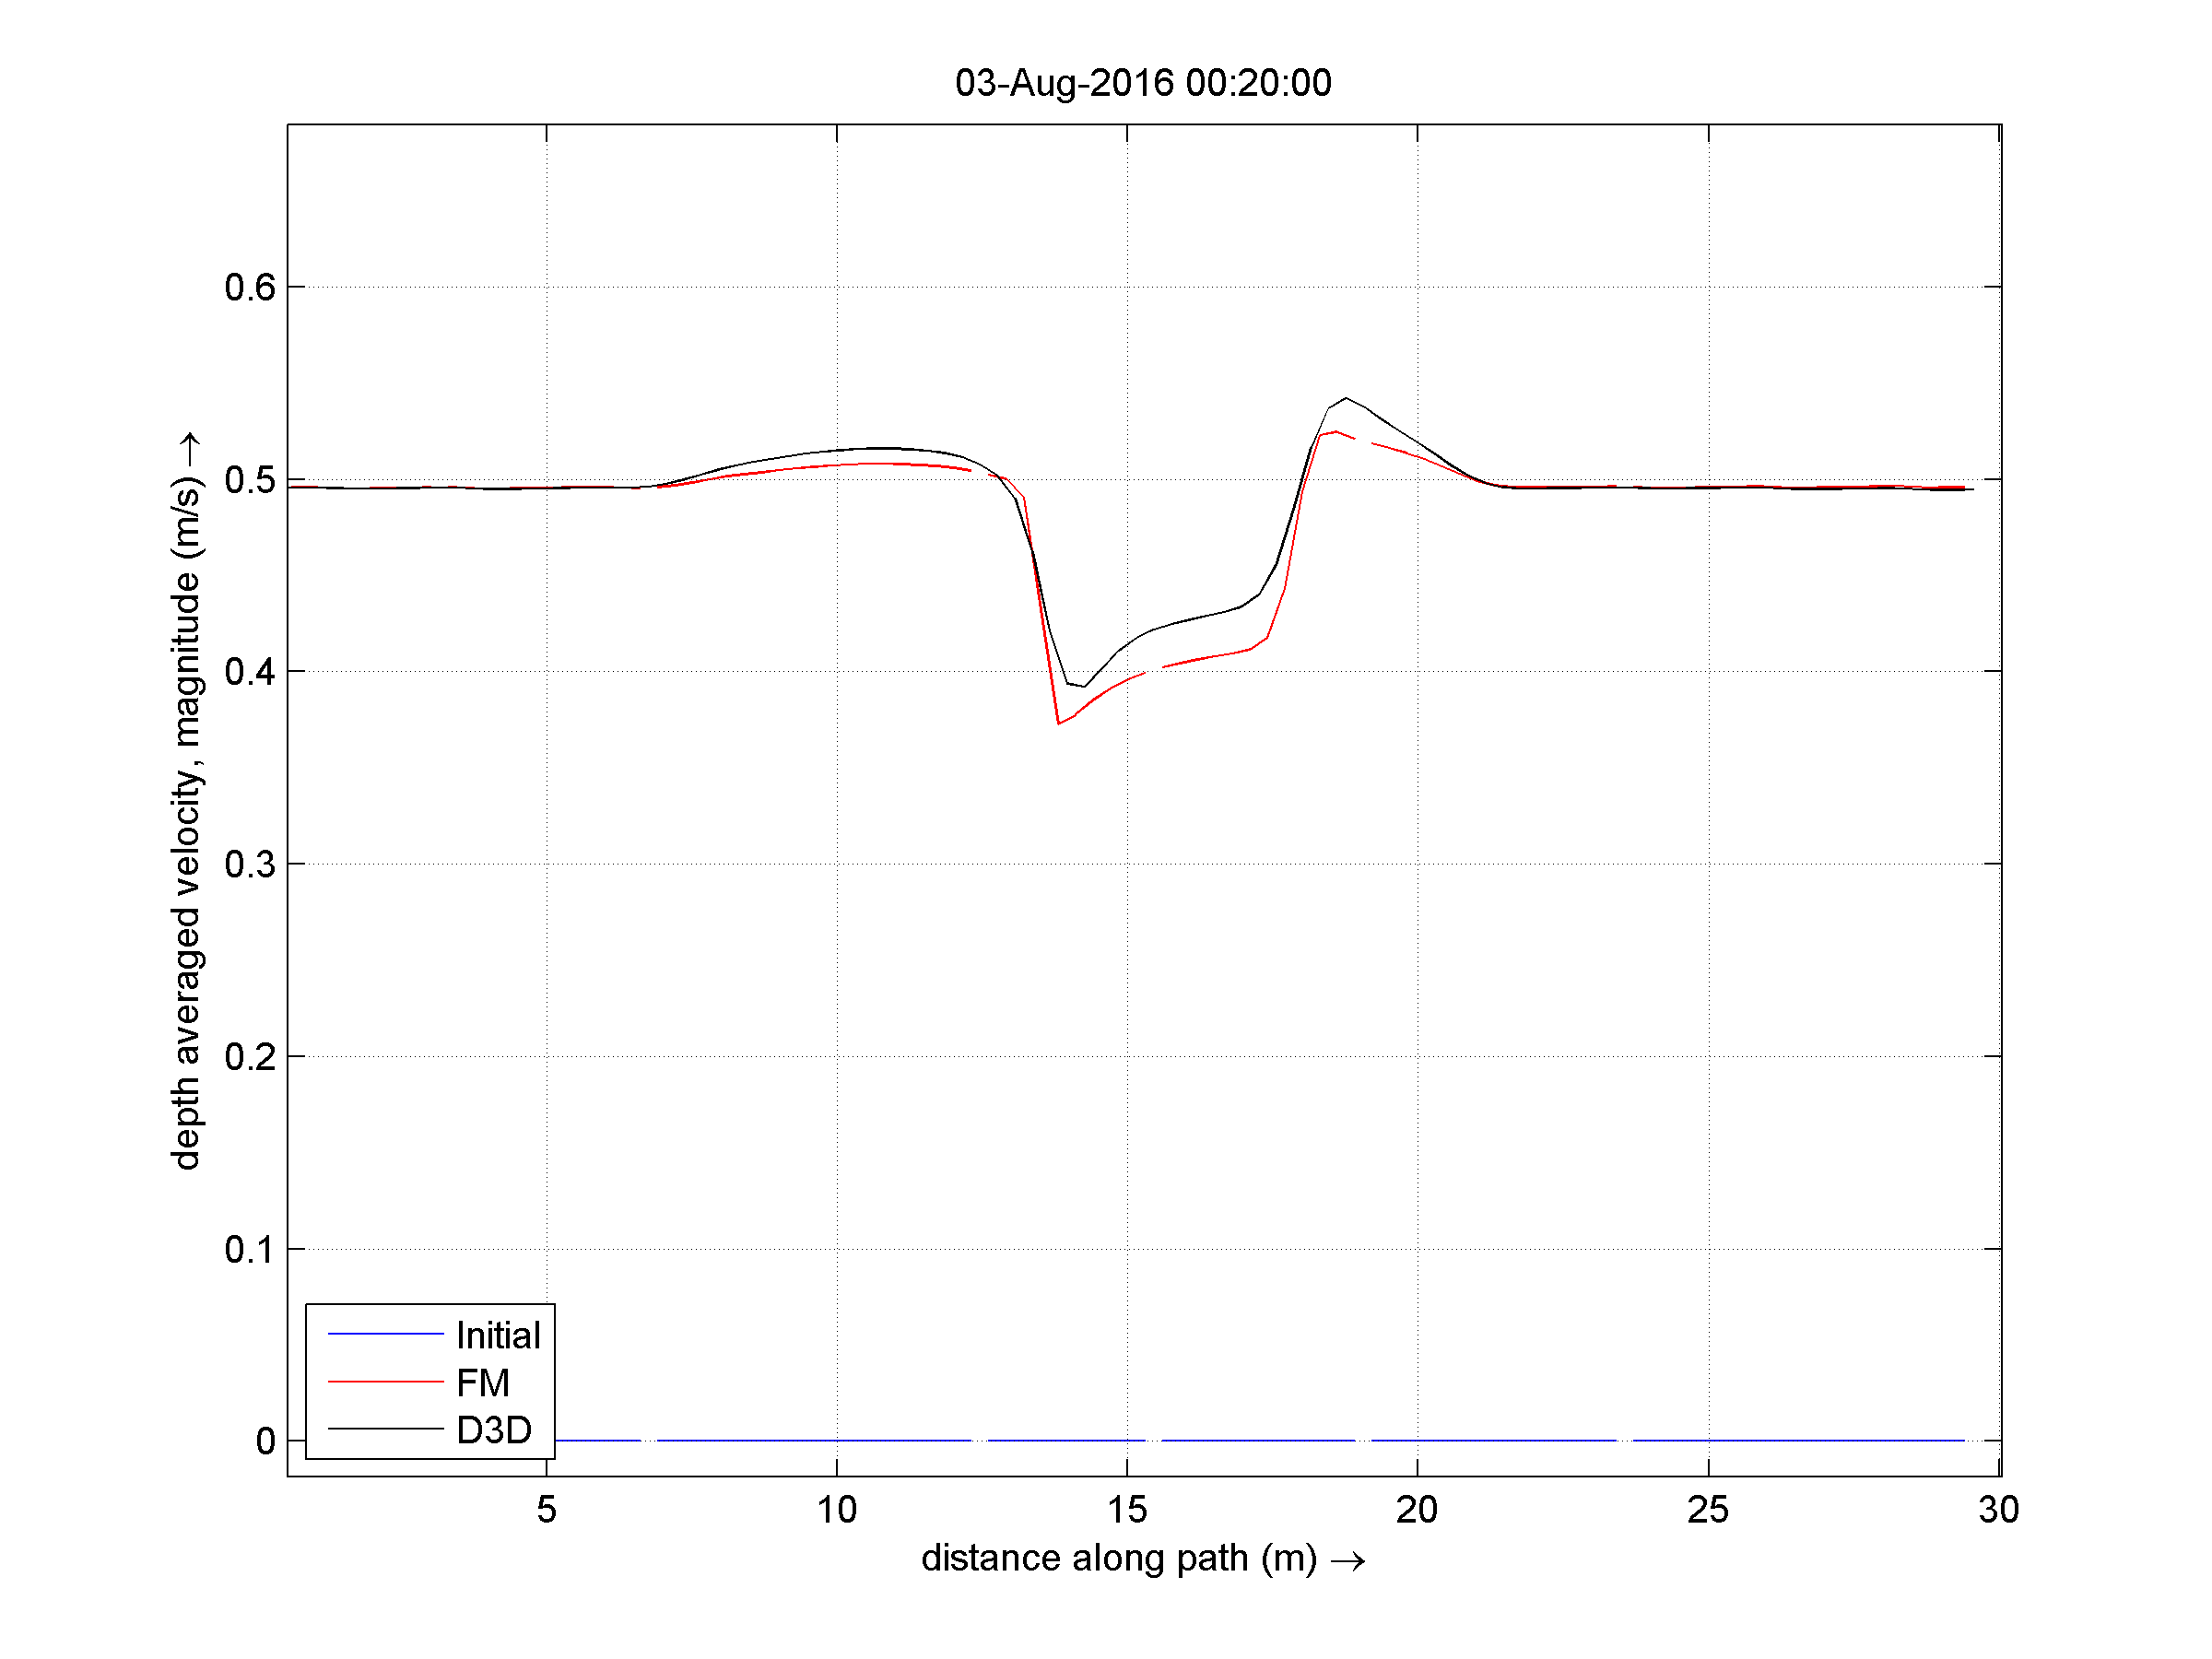
\includegraphics[width=0.7\columnwidth]{figures/C46velocityresult.png}
	\end{center}\caption{A comparison between FM and D3D: depth average velocity at the centerline of the channel after 20 minutes (C46)}
	\label{fig:C46V20min}
\end{figure}

\paragraph*{Results}
The dredging and dumping functions work well, if we use:
\begin{itemize}
	\item[$\bullet$] The dredge depth to control the dredging process.
	\item[$\bullet$] dumping inside the model, outside the model or distributes the dredged material in a various location in or outside the model including sand mining.
	\item[$\bullet$]  dredging and dumping functions  works with under layering. However, the magnitude of bed change is different , therefore it is recommended to compare FM  with Delft3D4  to see if the different in  results is also exist there.
\end{itemize}

Dredging and dumping are also worked well with graded and non-graded sediment. However, it is not possible to see how much  material is dredged per sediment fraction in the history file. This issue needs to be fixed.
In c39 we use a file to specify the sediment grain size in spatial distribution. Yet, the influence of this file cannot be seen in the output results file. Therefore, it is recommended to add some extra outputs to realize the effect of using variable grain size distribution.
The dredging volume is not available in the history file or might not be possible to see it through Quickplot. The sediment volume per area and type is very important to be one of the results. Since it is one of the  main interested outputs for the real application of dredging and dumping process in rivers and estuaries.
In addition the sediment nourishment function is also working well in FM (sed-more) software. The slight difference in the magnitude of bed change might need further investigation.
\paragraph*{Conclusion}
The dredging, dumping and nourishment functions in the sed-mor module of the flexible mesh are well working with respect to the above testing conditions. History file requires more development to be able to recognize the volumes; This may allow to have an accurate comparison between dredging and dumping under various conditions.
\paragraph*{Version}
These tests have been carried out using the following software versions:
\begin{itemize}
	\item[$\bullet$] dflow-fm-x64-1.1.188.46871 used in testing c35 to c45
	\item[$\bullet$] dflow-fm-x64-1.1.188.47116 used in testing c46 
	\item[$\bullet$] FLOW2D3D 6.01.07.3574 for all setup Delft3D simulations.
\end{itemize}

%------------------------------------------------------------------------------

